\documentclass[12pt]{article}

\usepackage[]{graphicx}
\usepackage[]{color}
\usepackage{alltt}
\usepackage{subcaption}
\usepackage{placeins}
\usepackage{float}
\usepackage{array}

\newcommand{\mytitle}{Predicting interactions between phages and bacteria
through proteome representation}
\newcommand{\mysubtitle}{A latent space approach across CRC, IBD and GvHD cohorts}
\newcommand{\myname}{Sinan Maximilian Klein}
\newcommand{\mysupervisor}{Christian L. M\"uller}
\newcommand{\mydate}{Munich, September 17\textsuperscript{th}, 2026}

\usepackage[a4paper, width = 160mm, top = 35mm, bottom = 30mm,
bindingoffset = 0mm]{geometry}
\usepackage[utf8]{inputenc}
\usepackage{amsmath}
\usepackage{amssymb}
\usepackage{ragged2e}
\usepackage{xcolor}
\usepackage[round, comma]{natbib}
\usepackage{fancyhdr}
\newcommand{\changefont}{%
    \fontsize{8}{11}\selectfont
}
\usepackage{tikz}
\usetikzlibrary{arrows.meta, positioning}
\usepackage{hyperref}
\hypersetup{
  colorlinks = true,
  linkcolor = black,
  urlcolor = black,
  citecolor = black}
\pagestyle{fancy}
\fancyhead{}
\fancyhead[R]{\changefont{Predicting phage--bacteria interactions through proteome representation}}
\fancyfoot{}
\fancyfoot[R]{\thepage}
\setlength{\headheight}{14.5pt}
\setlength{\parindent}{0pt}
\interfootnotelinepenalty = 10000

% ------------------------------------------------------------------------------
% MAIN -------------------------------------------------------------------------
% ------------------------------------------------------------------------------
\IfFileExists{upquote.sty}{\usepackage{upquote}}{}
\begin{document}

% FRONT PAGE -------------------------------------------------------------------

\begin{titlepage}
\begin{center}

\LARGE
Bachelor's Thesis

\vspace{0.5cm}

\rule{\textwidth}{1.5pt}
\LARGE
\textbf{\mytitle}
\rule{\textwidth}{1.5pt}

\vspace{0.35cm}

\large
\mysubtitle

\vspace{0.5cm}

\large
Department of Statistics \\
Ludwig-Maximilians-Universität München

\vfill

\Large
\textbf{\myname}

\vfill

\large
\mydate

\vfill


\includegraphics[width = 0.4\textwidth]{sigillum.png}

\vfill

\normalsize
Submitted in partial fulfillment of the requirements for the degree of B. Sc.
\\

Supervised by \mysupervisor

\end{center}
\end{titlepage}

% CONTENTS ---------------------------------------------------------------------

\pagenumbering{Roman}
\newpage

\begin{abstract}
This thesis studies whether two related network representations can be predicted from a common set of high-dimensional 
features and whether their predictive information can be captured in a shared representation. The problem is 
investigated in the context of phage--bacteria interaction networks, where one network is constructed from sequence-based 
CRISPR evidence and the other from abundance-based conditional associations.

We use sparse logistic regression, multilayer perceptrons and gradient-boosted 
trees to assess the linear and nonlinear predictability of both networks, compare single-head with shared 
representations, and use a shuffled-label control to test whether any advantage of joint learning is 
attributable to information from the second network or to the joint training procedure itself.

Across three microbiome cohorts, the CRISPR linkage is substantially more predictable than the glasso
edge, although the advantage of nonlinear over linear modelling is inconsistent across cohorts and model
families. In contrast, the glasso edge remains only weakly to 
moderately predictable, with little evidence that increased model flexibility resolves this limitation. A shared 
representation can support both predictions with little loss in CRISPR performance and small improvements for the 
glasso edge. However, these improvements persist when the CRISPR labels are shuffled, suggesting that they are more 
consistent with a regularization-like effect of joint training than with meaningful information transfer
between the two networks.



\end{abstract}

\newpage
\tableofcontents

\newpage
\listoffigures
\newpage
\listoftables
\newpage

% CHAPTERS ---------------------------------------------------------------------

\pagenumbering{arabic}

\section{Introduction}
\label{intro}
\subsection{Motivation and overview}
\label{intro:overview}
The human gut holds a dense bacterial community alongside a large population of the viruses that infect it,
most of them bacteriophages \citep{shkoporov2019}. Infection requires a match between molecular structures on
both partners, so a phage generally infects only a narrow range of hosts, and in removing some bacteria and
not others it shapes the community. Shifts in that composition have been associated with colorectal cancer,
inflammatory bowel disease and graft-versus-host disease \citep{wirbel2019,lloydprice2019,peled2020}. Which
phage infects which bacterium is therefore worth knowing, and is rarely observed directly.

Two proxies are available from sequencing data, and they are of different kinds. A CRISPR spacer is a fragment of viral DNA
stored in the bacterial genome, so a spacer matching a viral genome shows that the bacterium's lineage was
infected by that virus at some point in the past; the match itself is found computationally
\citep{zhang2021spacepharer}. A co-abundance network, on the other hand, is estimated statistically: a
graphical lasso over abundances measured across samples marks pairs whose abundances covary once every other
organism is held fixed \citep{friedman2008,liu2010}.

Computational host prediction is an established problem, but existing approaches build their features from
curated references and assign a host taxon to a phage \citep{edwards2016,coutinho2021,roux2023,nie2024}. This
thesis describes organisms only by protein clusters formed \emph{de novo} within each cohort, without
functional annotation, and predicts both proxies on the identical set of genus--vOTU pairs in three cohorts.
Since the two targets are meant to describe one phenomenon, it also asks whether a single latent
representation can serve both.


\subsection{Research questions and outline}
\label{intro:questions}
The thesis addresses three questions.

\begin{enumerate}
  \item Can CRISPR linkage between a bacterial genus and a vOTU be predicted from an annotation-free
        protein-cluster representation of the two organisms?
  \item Can a co-abundance edge between the same pair be predicted from the same representation?
  \item Does a latent representation trained on both targets serve either better than one trained on a single
        target?
\end{enumerate}

The contribution is a controlled comparison: both proxies are predicted from identical features, on identical
folds, over the identical set of pairs, in three independent cohorts, so any difference between them is a
difference between the targets and not between the data or the models.

Figure~\ref{fig:pipeline-overview} summarises that setup. Each bacterial genus and each vOTU is described by its
own annotation-free protein-cluster profile; the two profiles are combined into a single pair representation,
and one model maps that representation to both targets.

\begin{figure}[htbp]
  \centering
  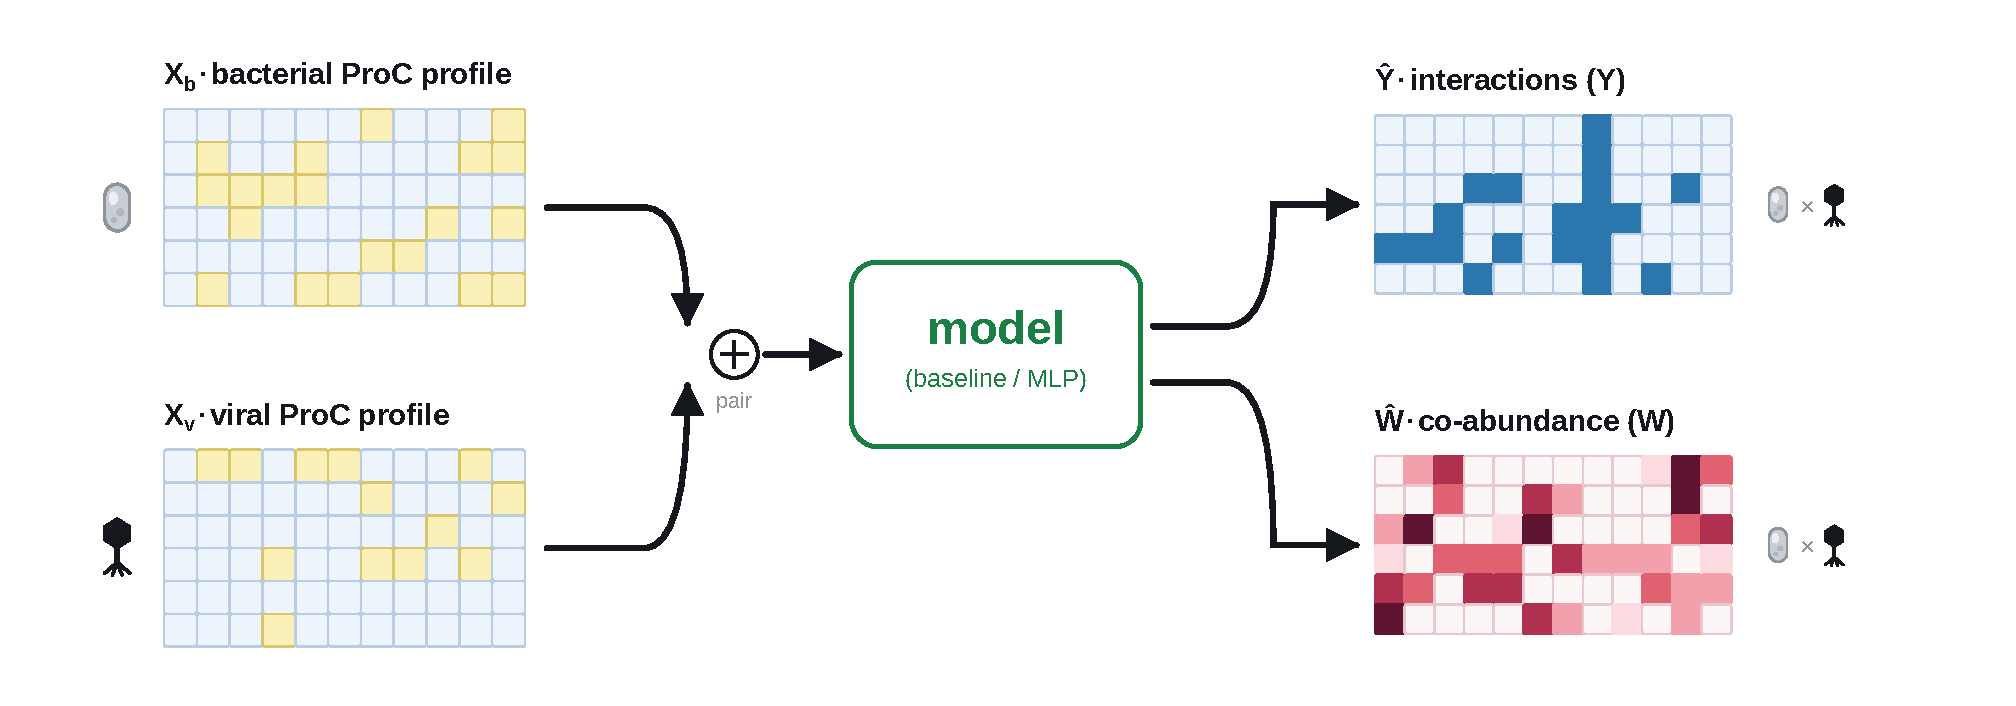
\includegraphics[width=\textwidth]{figures/fig_pipeline_overview.pdf}
  \caption{Overview of the prediction setup. A bacterial genus and a vOTU are each described by an
  annotation-free protein-cluster (ProC) profile, $X_b$ and $X_v$. The two profiles are combined into one
  pair representation, which a single model maps to both targets: CRISPR linkage $\hat{Y}$ and the glasso
  co-abundance edge $\hat{W}$. Both targets are predicted from the identical representation, on identical
  folds, over the identical set of genus--vOTU pairs. This figure was created by Claude Opus 5 (Anthropic).}
  \label{fig:pipeline-overview}
\end{figure}


\newpage

\section{Methods}
\label{methods}
\subsection{Problem Setup}

Let \(G=(\mathcal{B},\mathcal{V},E)\) be a bipartite graph with disjoint node sets
\(\mathcal{B}=\{b_1,\ldots,b_n\}\) and \(\mathcal{V}=\{v_1,\ldots,v_m\}\). Two networks are defined over
these node sets and built from different evidence: a binary network \(Y\in\{0,1\}^{n\times m}\) and a
weighted network \(W\in[0,1]^{n\times m}\). Each pair \((b_i,v_j)\) carries a feature vector
\(z_{ij}\in\mathbb{R}^{d}\).

The first model treats the two networks separately and conditions on the pair features. For each
network the conditional expectation given the features are,
\begin{equation}\label{eq:condmodels}
 \mu_{Y}(z)=\mathbb{E}\!\left[Y_{ij}\mid z_{ij}=z\right],
 \qquad
 \mu_{W}(z)=\mathbb{E}\!\left[W_{ij}\mid z_{ij}=z\right].
\end{equation}
We estimate each conditional expectation within a model class and test it on pairs held out from
fitting.

The second model is a joint prediction model where both networks are predicted from one representation of the same features,
\begin{equation}\label{eq:jointmodel}
 z_{ij}\;\longmapsto\;H_{ij}=h(z_{ij})\;\longmapsto\;\bigl(\widehat Y_{ij},\,\widehat W_{ij}\bigr),
 \qquad H_{ij}\in\mathbb{R}^{r},\quad r<d.
\end{equation}
The question is whether such a shared representation exists: whether the joint model matches the
separate ones in accuracy, and whether the representation it fits is common to both networks rather
than the one a single network induces on its own.

\subsection{General Analysis Pipeline}
\label{sec:pipeline}

The two node sets of the bipartite graph carry their own features:
\(X^{b}\in\mathbb{R}^{n\times d_b}\) holds the feature vectors of the nodes in \(\mathcal{B}\), one per
row, and \(X^{v}\in\mathbb{R}^{m\times d_v}\) those of the nodes in \(\mathcal{V}\). Write \(x^{b}_{i}\)
and \(x^{v}_{j}\) for the rows belonging to \(b_i\) and \(v_j\).

A transformation \(\varphi:\mathbb{R}^{d_b}\times\mathbb{R}^{d_v}\to\mathbb{R}^{d}\) maps the two node
vectors of a pair to a single pair vector,
\begin{equation}\label{eq:pairfeature}
 z_{ij}=\varphi\!\left(x^{b}_{i},x^{v}_{j}\right)\in\mathbb{R}^{d},
\end{equation}

Every pair \((i,j)\) in \(\mathcal{P}=\{1,\ldots,n\}\times\{1,\ldots,m\}\) therefore has a feature vector
\(z_{ij}\) and the two edge values \(Y_{ij}\) and \(W_{ij}\). Stacking over the \(nm\) pairs gives a design
matrix \(Z\in\mathbb{R}^{nm\times d}\) with one row per pair, together with the two networks vectorised into vectors of length
\(nm\).

The problem is then to find mappings from a row of \(Z\) to each edge value, and one mapping that produces both
from a single representation of that row. Figure~\ref{fig:setup} shows the construction.

\begin{figure}[htbp]
  \centering
  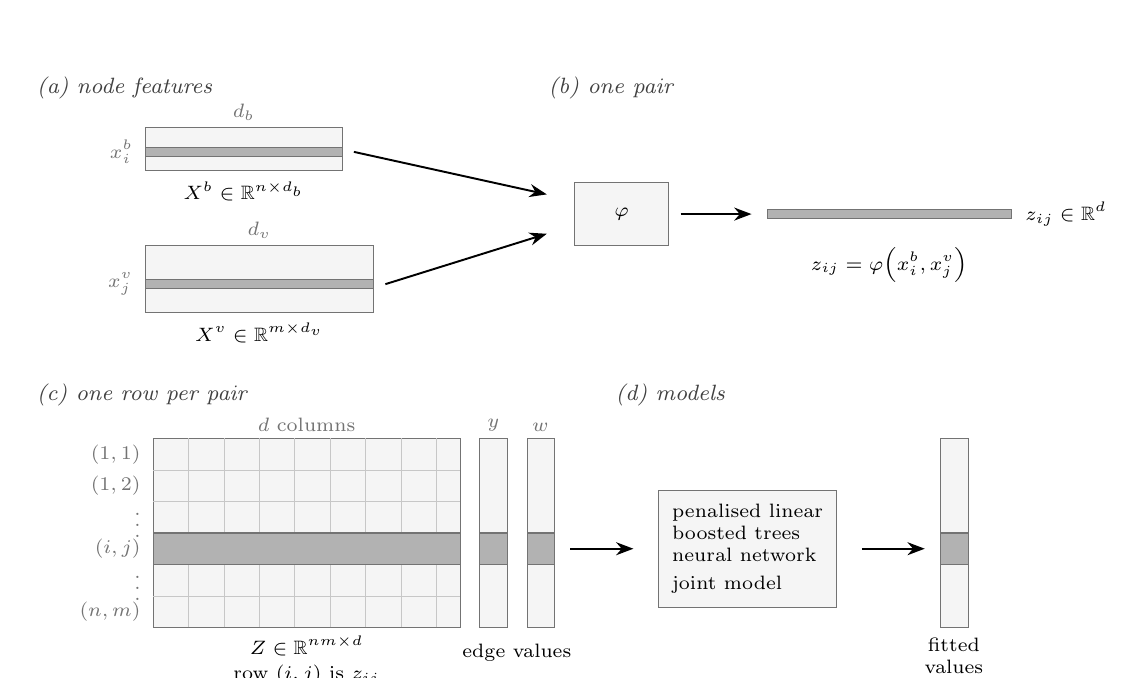
\begin{tikzpicture}[
      x = 1cm, y = 1cm, font = \small,
      mat/.style  = {draw = black!55, fill = black!4, line width = .4pt},
      hi/.style   = {draw = black!55, fill = black!30, line width = .4pt},
      gl/.style   = {black!22, line width = .3pt},
      arr/.style  = {-{Stealth[length = 2.2mm]}, line width = .7pt},
      dim/.style  = {font = \scriptsize, text = black!55, inner sep = 1.5pt},
      note/.style = {font = \scriptsize, inner sep = 2pt},
      stage/.style= {font = \footnotesize\itshape, anchor = west, text = black!75}
    ]

  % ---------- (a) node features ----------------------------------------
  \node[stage] at (0,3.55) {(a) node features};

  \draw[mat] (1.5,2.50) rectangle (4.0,3.05);
  \draw[hi]  (1.5,2.68) rectangle (4.0,2.80);
    \node[dim, left]   at (1.40,2.74) {$x^{b}_{i}$};
    \node[dim, above]  at (2.75,3.08) {$d_b$};
    \node[note, below] at (2.75,2.44) {$X^{b}\in\mathbb{R}^{n\times d_b}$};

  \draw[mat] (1.5,0.70) rectangle (4.4,1.55);
  \draw[hi]  (1.5,1.00) rectangle (4.4,1.12);
    \node[dim, left]   at (1.40,1.06) {$x^{v}_{j}$};
    \node[dim, above]  at (2.95,1.58) {$d_v$};
    \node[note, below] at (2.95,0.64) {$X^{v}\in\mathbb{R}^{m\times d_v}$};

  % ---------- (b) the transformation -----------------------------------
  \node[stage] at (6.5,3.55) {(b) one pair};

  \draw[arr] (4.15,2.74) -- (6.60,2.20);
  \draw[arr] (4.55,1.06) -- (6.60,1.70);
  \draw[mat, draw = black!55] (6.95,1.55) rectangle (8.15,2.35);
  \node[note] at (7.55,1.95) {$\varphi$};

  \draw[arr] (8.30,1.95) -- (9.20,1.95);
  \draw[hi] (9.40,1.89) rectangle (12.5,2.01);
    \node[note, right] at (12.6,1.95) {$z_{ij}\in\mathbb{R}^{d}$};
  \node[note] at (10.95,1.30) {$z_{ij}=\varphi\!\left(x^{b}_{i},x^{v}_{j}\right)$};

  % ---------- (c) design matrix ----------------------------------------
  \node[stage] at (0,-0.35) {(c) one row per pair};

  \draw[mat] (1.6,-3.30) rectangle (5.5,-0.90);
  \foreach \y in {-1.30,-1.70,...,-2.95} \draw[gl] (1.6,\y) -- (5.5,\y);
  \foreach \x in {2.05,2.50,...,5.20} \draw[gl] (\x,-3.30) -- (\x,-0.90);
  \draw[hi] (1.6,-2.50) rectangle (5.5,-2.10);
    \node[dim, above] at (3.55,-0.87) {$d$ columns};
    \node[dim, left]  at (1.50,-1.10) {$(1,1)$};
    \node[dim, left]  at (1.50,-1.50) {$(1,2)$};
    \node[dim, left]  at (1.50,-1.90) {$\vdots$};
    \node[dim, left]  at (1.50,-2.30) {$(i,j)$};
    \node[dim, left]  at (1.50,-2.70) {$\vdots$};
    \node[dim, left]  at (1.50,-3.10) {$(n,m)$};
  \node[note, align = center] at (3.55,-3.72)
        {$Z\in\mathbb{R}^{nm\times d}$\\[1pt] row $(i,j)$ is $z_{ij}$};

  \draw[mat] (5.75,-3.30) rectangle (6.10,-0.90);
    \node[dim, above] at (5.92,-0.87) {$y$};
  \draw[hi] (5.75,-2.50) rectangle (6.10,-2.10);
  \draw[mat] (6.35,-3.30) rectangle (6.70,-0.90);
    \node[dim, above] at (6.52,-0.87) {$w$};
  \draw[hi] (6.35,-2.50) rectangle (6.70,-2.10);
  \node[note] at (6.22,-3.62) {edge values};

  % ---------- (d) models ------------------------------------------------
  \node[stage] at (7.35,-0.35) {(d) models};

  \draw[arr] (6.90,-2.30) -- (7.70,-2.30);
  \node[mat, draw = black!55, align = left, inner sep = 5pt, font = \scriptsize]
        at (9.15,-2.30)
        {penalised linear\\ boosted trees\\ neural network\\[2pt] joint model};
  \draw[arr] (10.60,-2.30) -- (11.40,-2.30);

  \draw[mat] (11.60,-3.30) rectangle (11.95,-0.90);
  \draw[hi]  (11.60,-2.50) rectangle (11.95,-2.10);
    \node[note, below, align = center] at (11.77,-3.36) {fitted\\ values};

  \end{tikzpicture}
  \caption[Construction of the prediction problem]{Construction of the prediction problem. Each node
  carries a feature vector. For a pair \((b_i,v_j)\) the transformation \(\varphi\) combines the two node
  vectors into one pair vector \(z_{ij}\). Every pair contributes one row of the design matrix \(Z\), whose
  \(d\) columns are the coordinates of \(\varphi\); the two edge values are aligned with those rows. Each
  model maps a row to one fitted value.}
  \label{fig:setup}
\end{figure}
\FloatBarrier


\subsection{Models}
\label{sec:models}

\subsubsection{Baseline Models}

Every model maps one row \(z_{ij}\in\mathbb{R}^{d}\) to one value, and is fitted on a training index set
\(\mathcal{T}\subset\mathcal{P}\) and evaluated on \(\mathcal{P}\setminus\mathcal{T}\). For a binary edge value \(T_{ij}\in\{0,1\}\) the output is a fitted probability
\(\widehat p_{ij}\in(0,1)\); since the positive class is rare, each observation is weighted inversely to
the frequency of its class in \(\mathcal{T}\), giving weights \(\omega_{ij}>0\) and the weighted
cross-entropy
\begin{equation}\label{eq:bce}
 \ell(\theta)=-\sum_{(i,j)\in\mathcal{T}}\omega_{ij}
 \Bigl[T_{ij}\log\widehat p_{ij}(\theta)+\bigl(1-T_{ij}\bigr)\log\bigl(1-\widehat p_{ij}(\theta)\bigr)\Bigr].
\end{equation}
For a continuous edge value \(\widetilde W_{ij}\in\mathbb{R}\) the output \(\widehat{\widetilde W}_{ij}\) is
on the same scale and the criterion is the sum of squared errors
\begin{equation}\label{eq:sse}
 \mathrm{SSE}(\theta)=\sum_{(i,j)\in\mathcal{T}}
 \bigl(\widetilde W_{ij}-\widehat{\widetilde W}_{ij}(\theta)\bigr)^{2}.
\end{equation}
We use three model families, each in a classification and a regression variant.

\begin{itemize}

\item[--] \textbf{Penalised linear model.} For classification, \(L_{1}\)-penalised logistic regression
\citep{tibshirani1996}: with \(\beta\in\mathbb{R}^{d}\), \(\beta_{0}\in\mathbb{R}\) and
\(\sigma(u)=(1+e^{-u})^{-1}\), the output is \(\widehat p_{ij}=\sigma(\beta_{0}+z_{ij}^{\top}\beta)\) and
\begin{equation}\label{eq:lasso}
 \bigl(\widehat\beta_{0},\widehat\beta\bigr)
 =\operatorname*{arg\,min}_{\beta_{0},\beta}
 \Bigl\{\ell(\beta_{0},\beta)+\lambda\lVert\beta\rVert_{1}\Bigr\},
\end{equation}
and we select \(\lambda>0\) by an inner cross-validation on \(\mathcal{T}\) under the one-standard-error
rule. The \(L_{1}\) penalty sets most of the \(d\) coefficients to exactly zero. For regression, ridge 
regression \citep{hoerl1970}: the output is \(\widehat{\widetilde W}_{ij}=\beta_{0}+z_{ij}^{\top}\beta\) and
\begin{equation}\label{eq:ridge}
 \bigl(\widehat\beta_{0},\widehat\beta\bigr)
 =\operatorname*{arg\,min}_{\beta_{0},\beta}
 \Bigl\{\mathrm{SSE}(\beta_{0},\beta)+\alpha\lVert\beta\rVert_{2}^{2}\Bigr\},
 \qquad \alpha>0.
\end{equation}

\item[--] \textbf{Gradient-boosted trees.} The nonlinear tree model \citep{chen2016}, competitive on tabular feature
spaces \citep{grinsztajn2022}. From a constant \(f_{0}\), regression trees
\(\mathcal{T}_{t}:\mathbb{R}^{d}\to\mathbb{R}\) are fitted successively to the gradient of the criterion,
giving
\begin{equation}\label{eq:xgb}
 f(z)=f_{0}+\eta\sum_{t=1}^{n_{\mathrm{tree}}}\mathcal{T}_{t}(z),
\end{equation}
with \(n_{\mathrm{tree}}\) trees and learning rate \(\eta\in(0,1]\). For classification the trees are fitted to the gradient 
of the cross-entropy and the output is
\(\widehat p_{ij}=\sigma(f(z_{ij}))\) whereas for regression to the gradient of the squared-error criterion
and the output is \(\widehat{\widetilde W}_{ij}=f(z_{ij})\).

\item[--] \textbf{Neural network.} A single hidden layer of width \(r\) \citep{Bishop2006}. With
\(\Psi\in\mathbb{R}^{r\times d}\) and \(\psi\in\mathbb{R}^{r}\),
\begin{equation}\label{eq:mlp}
 H_{ij}=\mathrm{Drop}_{\rho}\!\Bigl(\mathrm{ReLU}\bigl(\Psi z_{ij}+\psi\bigr)\Bigr)\in\mathbb{R}^{r},
\end{equation}
where \(\mathrm{ReLU}(u)=\max(u,0)\) acts coordinatewise and \(\mathrm{Drop}_{\rho}\) zeroes each
coordinate independently with probability \(\rho\) during fitting and is the identity at prediction time.
A linear head with \(\phi\in\mathbb{R}^{r}\) and \(\phi_{0}\in\mathbb{R}\) follows: for classification
\(\widehat p_{ij}=\sigma(\phi^{\top}H_{ij}+\phi_{0})\), minimising the cross-entropy; for regression
\(\widehat{\widetilde W}_{ij}=\phi^{\top}H_{ij}+\phi_{0}\), minimising the squared-error criterion.

\end{itemize}





\subsubsection{Latent-Space Model}

The joint model uses the same hidden layer as the neural network above, but lets one representation feed
two heads. With \(\Psi\in\mathbb{R}^{r\times d}\) and \(\psi\in\mathbb{R}^{r}\),
\begin{equation}\label{eq:trunk}
 H_{ij}=\mathrm{Drop}_{\rho}\!\Bigl(\mathrm{ReLU}\bigl(\Psi z_{ij}+\psi\bigr)\Bigr)\in\mathbb{R}^{r},
\end{equation}
and since \(r<d\) this layer is a bottleneck: the \(d\) coordinates of \(z_{ij}\) are compressed to \(r\)
before either edge value is predicted. Two linear heads act on the same \(H_{ij}\),
\begin{equation}\label{eq:heads}
 \widehat p^{\,Y}_{ij}=\sigma\!\left(\phi_{Y}^{\top}H_{ij}+\phi_{0Y}\right),
 \qquad
 \widehat p^{\,W}_{ij}=\sigma\!\left(\phi_{W}^{\top}H_{ij}+\phi_{0W}\right),
\end{equation}
with \(\phi_{Y},\phi_{W}\in\mathbb{R}^{r}\) and \(\phi_{0Y},\phi_{0W}\in\mathbb{R}\).

Both edge values are binary in this model, so each head is scored by the weighted binary cross-entropy.
Writing \(T^{W}_{ij}\in\{0,1\}\) for the binarised edge weight and \(\theta\) for all parameters,
\begin{equation}\label{eq:bceY}
 \ell_{Y}(\theta)=-\sum_{(i,j)\in\mathcal{T}}\omega^{Y}_{ij}
 \Bigl[\,Y_{ij}\log\widehat p^{\,Y}_{ij}
 +\bigl(1-Y_{ij}\bigr)\log\bigl(1-\widehat p^{\,Y}_{ij}\bigr)\Bigr],
\end{equation}
\begin{equation}\label{eq:bceW}
 \ell_{W}(\theta)=-\sum_{(i,j)\in\mathcal{T}}\omega^{W}_{ij}
 \Bigl[\,T^{W}_{ij}\log\widehat p^{\,W}_{ij}
 +\bigl(1-T^{W}_{ij}\bigr)\log\bigl(1-\widehat p^{\,W}_{ij}\bigr)\Bigr],
\end{equation}
where the weights \(\omega^{Y}_{ij}\) and \(\omega^{W}_{ij}\) are formed separately for each network, as
above. We estimate all parameters by minimising the weighted sum
\begin{equation}\label{eq:joint}
 \mathcal{L}(\theta)=\gamma_{Y}\,\ell_{Y}(\theta)+\gamma_{W}\,\ell_{W}(\theta),
 \qquad \gamma_{Y},\gamma_{W}>0.
\end{equation}
Both terms depend on \(\Psi\) and \(\psi\), so the hidden layer receives gradient contributions from both
edge values and \(H_{ij}\) has to support both heads at once. The single-head neural network has the identical
hidden layer and differs only in that the second term is absent, so comparing the two isolates the cost of
sharing one representation. Figure~\ref{fig:latent} shows the model.


\begin{figure}[htbp]
  \centering
  \resizebox{\textwidth}{!}{%
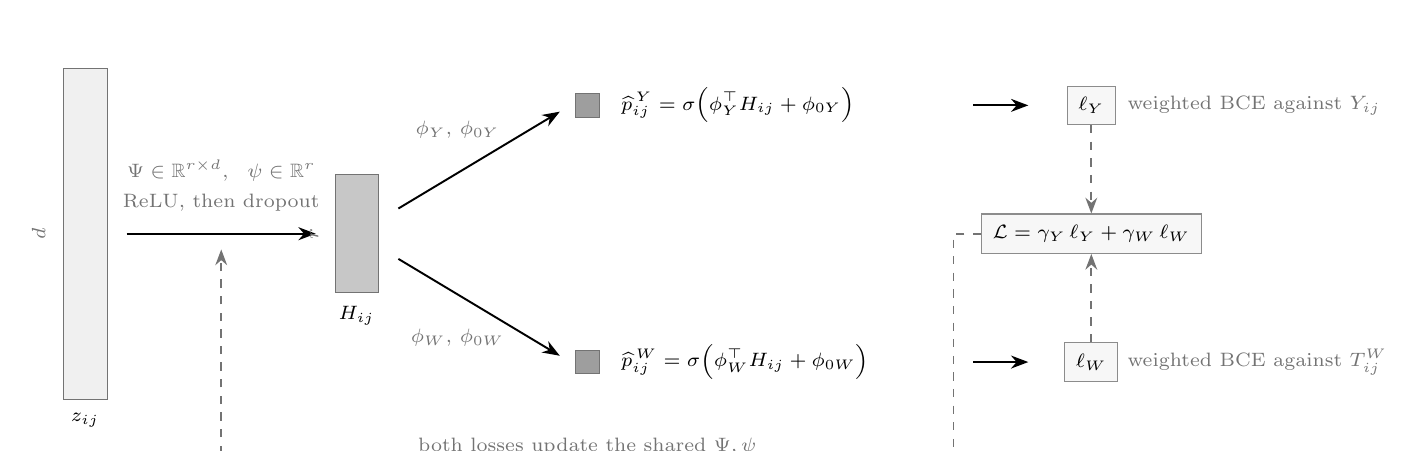
\begin{tikzpicture}[
      x = 1cm, y = 1cm, font = \small,
      bar/.style  = {draw = black!55, fill = black!6,  line width = .4pt},
      hid/.style  = {draw = black!55, fill = black!22, line width = .4pt},
      hdbox/.style= {draw = black!55, fill = black!38, line width = .4pt},
      arr/.style  = {-{Stealth[length = 2.2mm]}, line width = .7pt},
      grad/.style = {-{Stealth[length = 2mm]}, line width = .6pt, dashed, black!55},
      dim/.style  = {font = \scriptsize, text = black!55, inner sep = 1.5pt},
      note/.style = {font = \scriptsize, inner sep = 2pt}
    ]

  % input ---------------------------------------------------------------
  \draw[bar] (0,-2.10) rectangle (0.55,2.10);
    \node[dim, rotate = 90] at (-0.32,0) {$d$};
    \node[note, below] at (0.27,-2.20) {$z_{ij}$};

  % trunk ---------------------------------------------------------------
  \draw[arr] (0.80,0) -- (3.20,0);
    \node[dim, align = center] at (2.00,0.80)
          {$\Psi\in\mathbb{R}^{r\times d},\ \ \psi\in\mathbb{R}^{r}$};
    \node[dim, align = center] at (2.00,0.40) {$\mathrm{ReLU}$, then dropout};

  % shared representation ------------------------------------------------
  \draw[hid] (3.45,-0.75) rectangle (4.00,0.75);
    \node[dim, rotate = 90] at (3.18,0) {$r$};
    \node[note, below, align = center] at (3.72,-0.85) {$H_{ij}$};

  % two heads ----------------------------------------------------------
  \draw[arr] (4.25,0.32) -- (6.30,1.55);
    \node[dim] at (5.00,1.32) {$\phi_{Y},\,\phi_{0Y}$};
  \draw[arr] (4.25,-0.32) -- (6.30,-1.55);
    \node[dim] at (5.00,-1.32) {$\phi_{W},\,\phi_{0W}$};

  \draw[hdbox] (6.50,1.48) rectangle (6.80,1.78);
  \draw[hdbox] (6.50,-1.78) rectangle (6.80,-1.48);

  \node[note, right] at (7.00,1.63)
        {$\widehat p^{\,Y}_{ij}=\sigma\!\left(\phi_{Y}^{\top}H_{ij}+\phi_{0Y}\right)$};
  \node[note, right] at (7.00,-1.63)
        {$\widehat p^{\,W}_{ij}=\sigma\!\left(\phi_{W}^{\top}H_{ij}+\phi_{0W}\right)$};

  % losses -----------------------------------------------------------------
  \draw[arr] (11.55,1.63) -- (12.25,1.63);
  \draw[arr] (11.55,-1.63) -- (12.25,-1.63);
  \node[note, draw = black!45, fill = black!3, inner sep = 4pt] (ly) at (13.05,1.63)
        {$\ell_{Y}$};
  \node[note, draw = black!45, fill = black!3, inner sep = 4pt] (lw) at (13.05,-1.63)
        {$\ell_{W}$};
  \node[dim, right] at (13.45,1.63) {weighted BCE against $Y_{ij}$};
  \node[dim, right] at (13.45,-1.63) {weighted BCE against $T^{W}_{ij}$};

  \node[note, draw = black!45, fill = black!3, inner sep = 4pt] (loss) at (13.05,0)
        {$\mathcal{L}=\gamma_{Y}\,\ell_{Y}+\gamma_{W}\,\ell_{W}$};
  \draw[grad] (ly.south) -- (loss.north);
  \draw[grad] (lw.north) -- (loss.south);

  % shared gradient ----------------------------------------------------------
  \draw[grad] (loss.west) -- (11.30,0) -- (11.30,-2.90) -- (2.00,-2.90) -- (2.00,-0.20);
    \node[dim, above] at (6.65,-2.87) {both losses update the shared $\Psi,\psi$};

  \end{tikzpicture}%
}
  \caption[The shared-representation model]{The shared-representation model. A single hidden layer maps the
  pair vector \(z_{ij}\in\mathbb{R}^{d}\) to a representation \(H_{ij}\in\mathbb{R}^{r}\) with \(r<d\).
  Two linear heads act on the same \(H_{ij}\) and produce one probability each. Both are scored by a
  weighted binary cross-entropy, and the weighted sum of the two is minimised, so the hidden layer receives
  gradient contributions from both edge values.}
  \label{fig:latent}
\end{figure}
\FloatBarrier

\subsection{Training and Evaluation}
\label{sec:eval}

We partition the pairs \(\mathcal{P}\) once, before fitting any model, into \(F=10\) folds
\(\mathcal{P}_{1},\dots,\mathcal{P}_{F}\) of approximately equal size, stratified on \(Y\) and drawn from
a fixed seed. We fit each model on \(\mathcal{P}\setminus\mathcal{P}_{f}\) and score it on
\(\mathcal{P}_{f}\) for \(f=1,\dots,F\), and every model sees the identical partition. We centre and
scale each coordinate of \(Z\) using the mean and standard deviation of the training fold, except for the
tree ensembles, whose splits are invariant to monotone rescaling of a coordinate.

For the binary edge values we report the area under the receiver operating characteristic curve (AUC) and the
average precision (AP), the latter being the more informative of the two under strong class imbalance
\citep{davis2006}. Both are rank-based, so no decision threshold is applied to \(\widehat p_{ij}\). For
the weighted network we report the coefficient of determination on the original \([0,1]\) scale,
\begin{equation}\label{eq:r2}
 R^{2}_{f}
 =1-\frac{\sum_{(i,j)\in\mathcal{P}_{f}}\bigl(W_{ij}-\widehat W_{ij}\bigr)^{2}}
     {\sum_{(i,j)\in\mathcal{P}_{f}}\bigl(W_{ij}-\bar W_{f}\bigr)^{2}},
 \qquad
 \bar W_{f}=\frac{1}{|\mathcal{P}_{f}|}\sum_{(i,j)\in\mathcal{P}_{f}}W_{ij},
\end{equation}
so that \(R^{2}_{f}<0\) means the fitted values are worse on fold \(f\) than the constant prediction
\(\bar W_{f}\). We report every metric as a mean and a standard deviation over the \(F\) held-out folds. Two models are
compared by the mean of their per-fold differences and, where the consistency of a difference matters, by
the number of folds favouring each model. The training sets of different folds overlap, so a paired test
over the \(F\) differences has no unbiased variance estimator and its \(p\)-values would be
anti-conservative \citep{bengio2004}; we therefore report the differences themselves rather than a test.

\subsection{Representation Comparison}
\label{sec:cka}

Each of the three neural networks produces a hidden layer of width \(r\): write \(H^{Y}_{ij}\) and
\(H^{W}_{ij}\) for the layer of the single-head neural network fitted to \(Y\) and to the binarised edge
weight, and \(H^{YW}_{ij}\) for the shared layer of the joint model. Their coordinates cannot be
compared one by one, since an orthogonal transformation of a hidden layer together with a compensating
change of its head leaves every fitted value unchanged. What can be compared is the geometry each layer
induces on the pairs.

Let \(A\) and \(B\) hold two such layers evaluated on the same \(q\) pairs, stacked column-centred into
\(\mathbb{R}^{q\times r}\). Their linear centred kernel alignment \citep{kornblith2019} is
\begin{equation}\label{eq:cka}
 \operatorname{CKA}(A,B)
 =\frac{\bigl\lVert A^{\top}B\bigr\rVert_{F}^{2}}
       {\bigl\lVert A^{\top}A\bigr\rVert_{F}\,\bigl\lVert B^{\top}B\bigr\rVert_{F}}
 \;\in\;[0,1],
\end{equation}
which equals one when the two layers differ by an orthogonal transformation and a common scaling and is
invariant to both. It is not invariant to rescaling single coordinates, so we scale each coordinate to unit
variance before the comparison; otherwise a hidden unit with large activations would dominate the
alignment for no reason beyond its scale.

Every fold refits each neural network, so layers from different folds are not the same map and we do not
pool them. We compute the three pairwise values within each held-out fold \(\mathcal{P}_{f}\) and report
them as a mean and a standard deviation over the \(F\) folds.

\subsection{Robustness Analyses}
\label{sec:robustness}

We report two further analyses. The first asks whether a gain of the joint model on one network depends on information carried by the other; the second asks whether the
coordinates selected by the penalised linear model are stable under resampling.

\subsubsection{Permutation Control}
\label{sec:shuffley}

To separate a contribution of \(Y\) to the second head from the effect of joint fitting itself, the
we refit the joint model with the \(Y\) labels permuted within each training fold. Let
\(\varrho\) be a uniformly drawn permutation of \(\mathcal{T}\). We then fit the two heads against
\(Y_{\varrho(i,j)}\) and the unpermuted binarised edge weight respectively, with the representation
the hidden layer, the partition, the architecture, the hyperparameters and the random seed unchanged.
Under the permutation, \(Y_{\varrho(i,j)}\) is independent of \(z_{ij}\) by construction, so any
remaining gain on the second head cannot be attributed to information shared between the two
networks.

\subsubsection{Stability Selection}
\label{sec:stability}

To identify coordinates of \(z_{ij}\) that are selected consistently, we apply stability selection
\citep{meinshausen2010} to \(Y\). We resample over nodes rather than over pairs, because two pairs
sharing a node are not independent. For resample \(s\) we draw subsets
\(\mathcal{B}^{(s)}\subset\mathcal{B}\) and \(\mathcal{V}^{(s)}\subset\mathcal{V}\) containing half the
nodes of each set, and the resample consists of the observed pairs they span,
\begin{equation}\label{eq:subsample}
 \mathcal{P}^{(s)}=\bigl\{(i,j)\in\mathcal{P}\;:\;b_{i}\in\mathcal{B}^{(s)},\;v_{j}\in\mathcal{V}^{(s)}\bigr\}.
\end{equation}
Drawing \(K\) complementary pairs \citep{shah2013} gives \(S=2K\) resamples; we redraw a resample with fewer
than five positive \(Y_{ij}\).

Before resampling we remove coordinates that are non-zero in fewer than ten observed pairs or constant over
them, which leaves \(d\) candidate coordinates.

On each resample we centre and scale every coordinate within that resample and fit the
\(L_{1}\)-penalised logistic regression of Equation~\eqref{eq:lasso}, with class weights formed as in
Section~\ref{sec:models}, along the decreasing grid of penalties
\begin{equation}\label{eq:ssgrid}
 \lambda_{t}=\lambda_{\max}\,0.01^{(t-1)/29},\qquad t=1,\ldots,30,
\end{equation}
where \(\lambda_{\max}\) is the smallest penalty at which no coordinate is selected. The path of resample
\(s\) stops at the first penalty \(\lambda^{(s)}\) at which at least \(q\) coordinates are selected, and
\(\widehat S^{(s)}=\{k:\widehat\beta_{k}(\lambda^{(s)})\neq0\}\) records them. The selection probability
of coordinate \(k\) is estimated by the selection frequency
\begin{equation}\label{eq:pisel}
 \widehat\pi_{k}
 =\frac{1}{S}\sum_{s=1}^{S}\mathbf{1}\!\left\{k\in\widehat S^{(s)}\right\},
\end{equation}
and a coordinate is called stable when \(\widehat\pi_{k}\geq\pi_{\mathrm{thr}}\) for a threshold
\(\pi_{\mathrm{thr}}\in(\tfrac{1}{2},1)\). Under the exchangeability assumption of
\citet{meinshausen2010}, the expected number \(V\) of falsely selected coordinates satisfies
\begin{equation}\label{eq:mbbound}
 \mathbb{E}[V]\;\leq\;\frac{\bar q^{\,2}}{\left(2\pi_{\mathrm{thr}}-1\right)d},
\end{equation}
where \(\bar q\) is the average number of coordinates selected per resample. Requiring
\(\mathbb{E}[V]\leq1\) gives the target support size
\begin{equation}\label{eq:qbound}
 q=\left\lfloor\sqrt{\left(2\pi_{\mathrm{thr}}-1\right)d}\right\rfloor,
\end{equation}
at which each path is stopped. Because the grid is discrete, a resample can select slightly more than
\(q\) coordinates, so \(\bar q\) can exceed \(q\). Because the resampling draws nodes rather than
independent observations, we use the bound as a guide to the operating point rather than as an exact
error guarantee.

The penalty and class weighting are those of the penalised linear model of Section~\ref{sec:models}, but
the penalty is set by the stopping rule rather than by cross-validation, so the analysis describes the
coordinates that model class selects.


\newpage

\section{Data}
\label{data}
\subsection{Data Sources}
\label{data:sources}
The data come from three published studies of the human gut microbiome, covering colorectal cancer (CRC)
\citep{wirbel2019}, inflammatory bowel disease (IBD) \citep{lloydprice2019} and graft-versus-host disease
(GvHD) \citep{peled2020}. Their clinical endpoints play no role here. What each study contributes is a set
of bacterial genera, a set of viral operational taxonomic units (vOTUs), and abundance and protein
profiles for both, measured in the same samples.

The CRC data derive from \citet{wirbel2019}, a meta-analysis of eight faecal metagenomic studies of colorectal
cancer conducted in Germany, China, the United States and Japan, covering 768 cases together with controls. Of
these, 84 samples carry paired bacterial and viral measurements and enter this thesis.

The IBD data derive from \citet{lloydprice2019}, a longitudinal study of 132 subjects with Crohn's disease,
with ulcerative colitis, or without inflammatory bowel disease, each followed for one year at up to 24 time
points. Of the specimens collected there, 148 samples enter this thesis.

The GvHD data derive from \citet{peled2020}, a study of 1,362 patients undergoing allogeneic
haematopoietic-cell transplantation at four centres in New York, North Carolina, Germany and Japan, from which
8,767 faecal samples were collected. Of these, 90 samples enter this thesis.

Each cohort provides four tables: abundances for the bacterial genera and for the vOTUs, a spacer table
indexed by genus and by vOTU, and the protein profiles of both. We report their sizes with the other
descriptive quantities in the results.

Write \(\mathcal{B}=\{b_1,\ldots,b_n\}\) for the bacterial genera and
\(\mathcal{V}=\{v_1,\ldots,v_m\}\) for the vOTUs of a cohort that carry both a protein profile and an
abundance profile. Both networks below are indexed by the same candidate pairs, the Cartesian product
\begin{equation}\label{eq:pairs}
  \mathcal{P}=\mathcal{B}\times\mathcal{V},
\end{equation}
so a pair \((b_i,v_j)\) is one element of \(\mathcal{P}\) regardless of which network is being described.

\subsection{Protein Clusters}
\label{sec:mmseqs}

Individual protein sequences do not give a common vocabulary across organisms, so we first group similar
sequences into protein clusters with MMseqs2 \citep{steinegger2017}. MMseqs2 prefilters candidate
sequence pairs, aligns the kept candidates, and clusters those that are sufficiently similar; the same
prefilter-then-align strategy is used by other large-scale protein aligners \citep{buchfink2021}.

The clusters give one protein-count matrix per node set,
\[
  X^{b}\in\mathbb{R}^{n\times d_b},
  \qquad
  X^{v}\in\mathbb{R}^{m\times d_v},
\]
whose rows are organisms and whose columns are clusters; entry \((i,k)\) is the number of proteins of
organism \(i\) assigned to cluster \(k\). The two vocabularies are built separately and are of very
different size, so they do not share coordinates.

\subsection{Pair Feature}
\label{sec:phi}

The transformation \(\varphi\) of Section~\ref{sec:pipeline} maps the profiles \(x^{b}_{i}\) and
\(x^{v}_{j}\) of the two nodes of a pair to a single vector \(z_{ij}\in\mathbb{R}^{d}\). We fix it once,
before fitting any model, and use the same transformation for every model and both networks.

We use the protein clusters that occur in both vocabularies,
\(S=S^{\mathrm{all}}_{b}\cap S^{\mathrm{all}}_{v}\), so that coordinate \(k\) is the same cluster for the
bacterium and for the vOTU. We reduce the counts to presence,
\(\operatorname{bin}(x)_k=\mathbf{1}\{x_k>0\}\), which is invariant to per-organism rescaling and
therefore unaffected by proteome size or assembly completeness, and add the two halves coordinatewise,
\begin{equation}\label{eq:phi}
  z_{ij}=\operatorname{bin}\!\bigl(x^{b}_{i,S}\bigr)+\operatorname{bin}\!\bigl(x^{v}_{j,S}\bigr)
  \;\in\;\{0,1,2\}^{d}.
\end{equation}
So \(z_{ij,k}\) counts how many of the two partners carry cluster \(k\): none, one, or both. 

\subsection{CRISPR Network}
\label{sec:crispr}
If the spacers of a bacterium are compared against the genomes of viruses, a sufficiently strong match provides 
evidence that the bacterium, or a related bacterial lineage, has previously encountered the corresponding virus 
or a closely related virus. The absence of a match, however, does not establish the opposite.

One of the main issues is that CRISPR spacers are only around 30 nucleotides long, so standard nucleotide 
searches can lose sensitivity, especially when the viral sequence has diverged from the sequence from which the 
spacer was originally acquired. SpacePHARER \citep{zhang2021spacepharer} addresses this by translating both 
CRISPR spacers and viral genomes in all six reading frames and comparing the resulting sequences at the protein 
level. Candidate hits are subsequently realigned at the nucleotide level. SpacePHARER then combines the evidence 
from multiple spacers of one bacterium against the same viral genome into a single score and controls the 
resulting matches using a false discovery rate threshold. The search was run separately for each cohort, and 
its output enters as the CRISPR table of Section~\ref{data:sources}.

Only bacteria carrying a CRISPR--Cas system produce spacers, the occurrence of such systems differs between
taxonomic groups, and spacers are lost over evolutionary time. An interaction leaving no spacer record is
therefore indistinguishable from one that never occurred, and \(Y\) records sequence-supported historical
relationships rather than all interactions.


The network is defined over all of \(\mathcal{P}\), with \(Y_{ij}=1\) when the search reports CRISPR
evidence for the pair \((b_i,v_j)\) and \(Y_{ij}=0\) otherwise.

\subsection{Abundance Network}

Marginal association between two taxa can be induced by a third, so the network is defined by conditional
association instead. For variables \(a=(a_1,\ldots,a_P)\) with covariance \(\Sigma\), the precision matrix
\(\Theta=\Sigma^{-1}\) satisfies \(\Theta_{k\ell}=0\) exactly when \(a_k\) and \(a_\ell\) are
conditionally independent given all remaining variables, under a Gaussian assumption \citep{Bishop2006}.
Its non-zero off-diagonal entries are the edges of the network.

SPIEC-EASI \citep{kurtz2015} estimates such a network from compositional abundance data in three steps.
The abundance matrix \(C\in\mathbb{R}_{\geq0}^{N\times P}\) of \(N\) samples and \(P\) variables is first
centred-log-ratio transformed \citep{aitchison1982},
\(\tilde c_{sk}=\log c_{sk}-P^{-1}\sum_{\ell}\log c_{s\ell}\). Its precision matrix is then estimated
under an \(L_{1}\) penalty by the graphical lasso \citep{friedman2008},
\begin{equation}\label{eq:glasso}
  \widehat\Theta_{\lambda}
  =\operatorname*{arg\,min}_{\Theta\succ0}
  \Bigl\{\operatorname{tr}\bigl(\widehat\Sigma\Theta\bigr)-\log\det\Theta
  +\lambda\textstyle\sum_{k\neq\ell}\lvert\Theta_{k\ell}\rvert\Bigr\},
\end{equation}
where a larger \(\lambda\) gives a sparser network. Finally \(\lambda\) is chosen by StARS
\citep{liu2010}: the estimate is refitted on \(B\) subsamples, the selection frequency of an edge is
\begin{equation}\label{eq:stars-pi}
  \widehat\pi^{\,\mathrm{gl}}_{k\ell}(\lambda)
  =\frac{1}{B}\sum_{r=1}^{B}
  \mathbf{1}\bigl\{\widehat\Theta^{(r)}_{\lambda,k\ell}\neq0\bigr\},
\end{equation}
and \(\widehat\lambda_{\mathrm{StARS}}\) is the least regularised value at which the average edge
instability \(2\widehat\pi^{\,\mathrm{gl}}(1-\widehat\pi^{\,\mathrm{gl}})\) stays below a threshold
\(\xi^{\ast}\). We apply SPIEC-EASI to each cohort separately with \(\xi^{\ast}=0.02\) rather than the
standard \(0.05\), since the selected network is unstable at less conservative thresholds.

The abundance table stacks both domains, so \(P=n+m\) and \(\widehat\Theta\) is one symmetric
\((n+m)\times(n+m)\) matrix with three blocks,
\begin{equation}\label{eq:blocks}
  \widehat\Theta=
  \begin{pmatrix}
    \widehat\Theta^{\,\mathcal{B}\mathcal{B}} & \widehat\Theta^{\,\mathcal{B}\mathcal{V}}\\[2pt]
    \bigl(\widehat\Theta^{\,\mathcal{B}\mathcal{V}}\bigr)^{\!\top} & \widehat\Theta^{\,\mathcal{V}\mathcal{V}}
  \end{pmatrix},
  \qquad
  \widehat\Theta^{\,\mathcal{B}\mathcal{V}}\in\mathbb{R}^{n\times m},
\end{equation}
of which we keep only the off-diagonal block and discard the within-domain ones. The estimated network is
therefore not bipartite but a rectangular sub-block of a conditional-dependence network over all \(n+m\)
taxa, and a kept entry describes a conditional dependence given every other taxon, including those whose
blocks are dropped.

The weighted network is not an entry of \(\widehat\Theta\) but the StARS selection frequency of the
corresponding cross-block edge at the selected penalty. Writing \(k(i)\) and \(\ell(j)\) for the indices
of \(b_i\) and \(v_j\) among the \(P\) variables,
\begin{equation}\label{eq:Wdef}
  W_{ij}
  =\widehat\pi^{\,\mathrm{gl}}_{k(i)\,\ell(j)}\bigl(\widehat\lambda_{\mathrm{StARS}}\bigr)\in[0,1],
\end{equation}
so \(W_{ij}\) is the proportion of subsamples in which that edge was selected: a measure of how
reproducibly the edge is recovered, not a partial correlation or a precision entry.

\subsection{Missing Values and \(W\) Binarisation}
\label{sec:mask}

The two networks are constructed independently and do not span the same nodes. The CRISPR network is
defined over all of \(\mathcal{P}\), whereas the abundance network covers only the taxa that entered
SPIEC-EASI, so \(W\) is missing for the remaining pairs. With
\(\mathcal{B}_W\subseteq\mathcal{B}\) and \(\mathcal{V}_W\subseteq\mathcal{V}\) the nodes it contains,
\begin{equation}\label{eq:maskdef}
  M_{ij}=\mathbf{1}\{b_i\in\mathcal{B}_W\}\,\mathbf{1}\{v_j\in\mathcal{V}_W\},
  \qquad
  \mathcal{O}=\bigl\{(i,j)\in\mathcal{P}:M_{ij}=1\bigr\},
\end{equation}
and pairs outside \(\mathcal{O}\) are missing values of \(W\) rather than absent edges. The indicator
factorises into a row term and a column term, so whether a pair is observed is determined by its two
nodes alone and not by the value of \(W\). We fit and evaluate every model on \(\mathcal{O}\), a complete-case
analysis, so the design matrix has \(|\mathcal{O}|\) rows rather than \(nm\).

\paragraph{\(W\) Binarisation}
For binary prediction, thresholding at \(\tau\in[0,1)\) gives
\begin{equation}\label{eq:thresh}
  W^{(\tau)}_{ij}=\mathbf{1}\{W_{ij}>\tau\},
\end{equation}
so \(W^{(0)}_{ij}\) marks every pair selected in at least one subsample and a larger \(\tau\) demands a
more reproducibly selected edge. We use \(\tau=0\) in all later analyses. This is the natural cut between
an edge that is never selected and one that is selected at all, it requires no tuning, and it leaves a
near-balanced split between the two classes, whereas a larger \(\tau\) leaves too few positive pairs to
fit. In continuous form \(W_{ij}\) is bounded while the regression models predict on the real line, so we
fit on a logit scale and map back before scoring: we clip values to \([\varepsilon,1-\varepsilon]\) with
\(\varepsilon=10^{-3}\), transform by \(\widetilde W_{ij}=\operatorname{logit}(\cdot)\), and return the
fitted values as \(\widehat W_{ij}=\sigma(\widehat{\widetilde W}_{ij})\), against which we compute
\(R^{2}\) on the original scale.

\subsection{Model Hyperparameters}

The model and optimization hyperparameters are summarized in Table~\ref{tab:model_hyperparameters}. Both neural models are
regularized with dropout \citep{srivastava2014} and trained with the AdamW optimizer \citep{loshchilov2019}.

\begin{table}[htbp]
\centering
\caption{Hyperparameters used for the baseline and latent-space models.}
\label{tab:model_hyperparameters}
\begin{tabular}{lll}
\hline
\textbf{Model} & \textbf{Hyperparameter} & \textbf{Value} \\
\hline

Sparse logistic regression
& penalty & \(L_1\) \\
& regularization & selected by 3-fold CV \\
& selection rule & one-standard-error rule \\
& solver & liblinear \\
& maximum iterations & 2000 \\
& class weighting & balanced \\
\hline

Ridge regression
& \(L_2\) penalty \(\alpha\) & 1.0 \\
\hline

XGBoost classifier
& number of trees & 500 \\
& maximum tree depth & 4 \\
& learning rate & 0.05 \\
& row subsampling & 0.8 \\
& feature subsampling & 0.8 \\
& class weighting & \(n_{\mathrm{neg}}/n_{\mathrm{pos}}\) \\
\hline

XGBoost regression
& number of trees & 500 \\
& maximum tree depth & 4 \\
& learning rate & 0.05 \\
& row subsampling & 0.8 \\
& feature subsampling & 0.8 \\
\hline

MLP classifier/regressor
& hidden dimension & 64 \\
& activation & ReLU \\
& dropout & 0.3 \\
& batch size & 512 \\
& optimizer & AdamW \\
& learning rate & \(3\times10^{-4}\) \\
& weight decay & \(10^{-3}\) \\
& epochs & 200 \\
\hline

Joint latent model
& joint latent dimension & 64 \\
& head weights & \(\gamma_Y=\gamma_W=1\) \\
& activation & ReLU \\
& dropout & 0.3 \\
& batch size & 512 \\
& optimizer & AdamW \\
& learning rate & \(3\times10^{-4}\) \\
& weight decay & \(10^{-3}\) \\
& epochs & 200 \\
\hline
\end{tabular}
\end{table}
\FloatBarrier

\newpage

\section{Results}
\label{results}
\subsection{Protein Clusters}
Table~\ref{tab:procs} gives the dimensions of the two protein-cluster matrices and how densely they are
filled. Both are sparse, but the viral matrix more so than the bacterial one.

\begin{table}[htbp]
  \centering
  \caption{Protein-cluster matrices, by cohort}
  \label{tab:procs}
  \begin{tabular}{lrrr}
    \hline
                                  &    CRC &    IBD &   GvHD \\
    \hline
    \multicolumn{4}{l}{\textit{Bacteria}} \\
    Genera profiled               &    296 &    285 &    311 \\
    Protein clusters              & 70,625 & 78,517 & 72,646 \\
    Density of $X^{b}$            & 4.38\% & 4.29\% & 4.28\% \\
    Median clusters per genus     &  2,164 &  2,232 &  2,168 \\
    \hline
    \multicolumn{4}{l}{\textit{Viruses}} \\
    vOTUs profiled                &    573 &    692 &    906 \\
    Contigs                       &  6,876 &  8,045 &  5,101 \\
    Median contigs per vOTU       &      3 &      5 &      2 \\
    Protein clusters              &  2,756 &  4,226 &  7,168 \\
    Density of $X^{v}$            & 0.90\% & 0.82\% & 0.76\% \\
    Median clusters per vOTU      &     16 &     20 &     45 \\
    \hline
  \end{tabular}
\end{table}
\FloatBarrier

Figures~\ref{fig:procsparsity-crc} to~\ref{fig:procsparsity-gvhd} show the sparsity of the two
protein-cluster matrices in each cohort.

\begin{figure}[htbp]
  \centering
  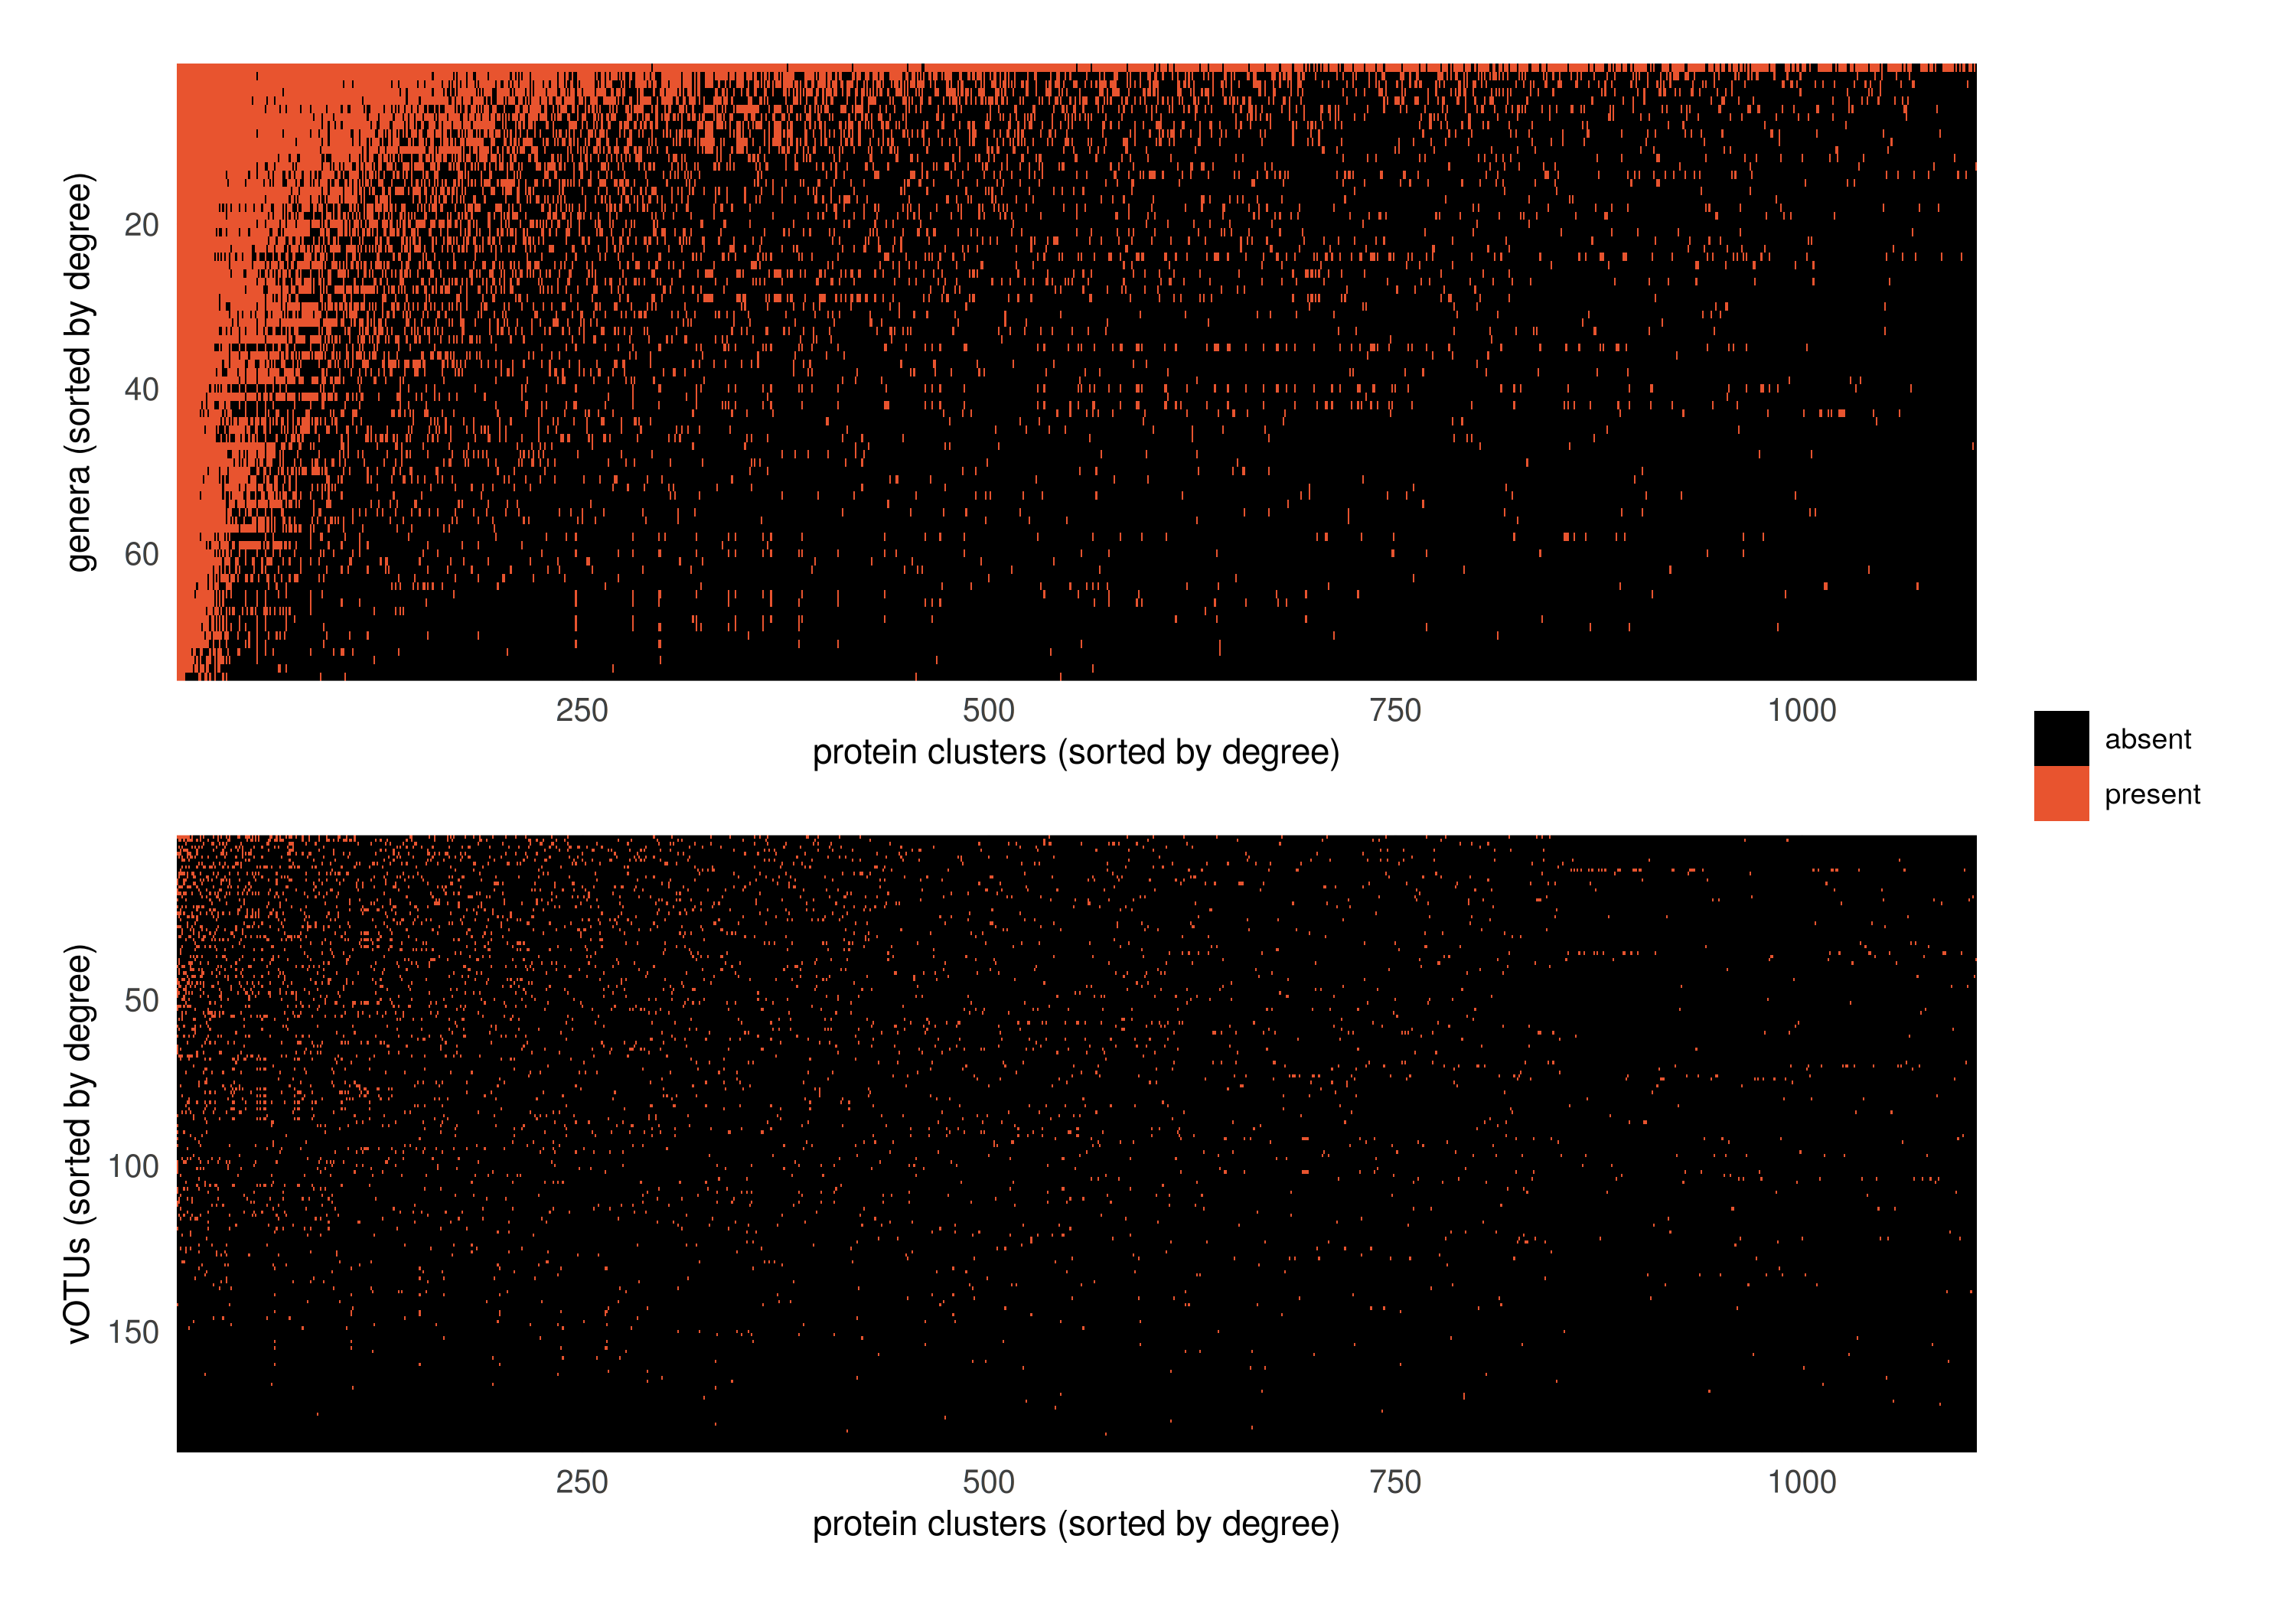
\includegraphics[width=0.88\textwidth]{figures/fig_procsparsity_crc.png}
  \caption{Protein-cluster sparsity, CRC}
  \label{fig:procsparsity-crc}
\end{figure}
\FloatBarrier

\begin{figure}[htbp]
  \centering
  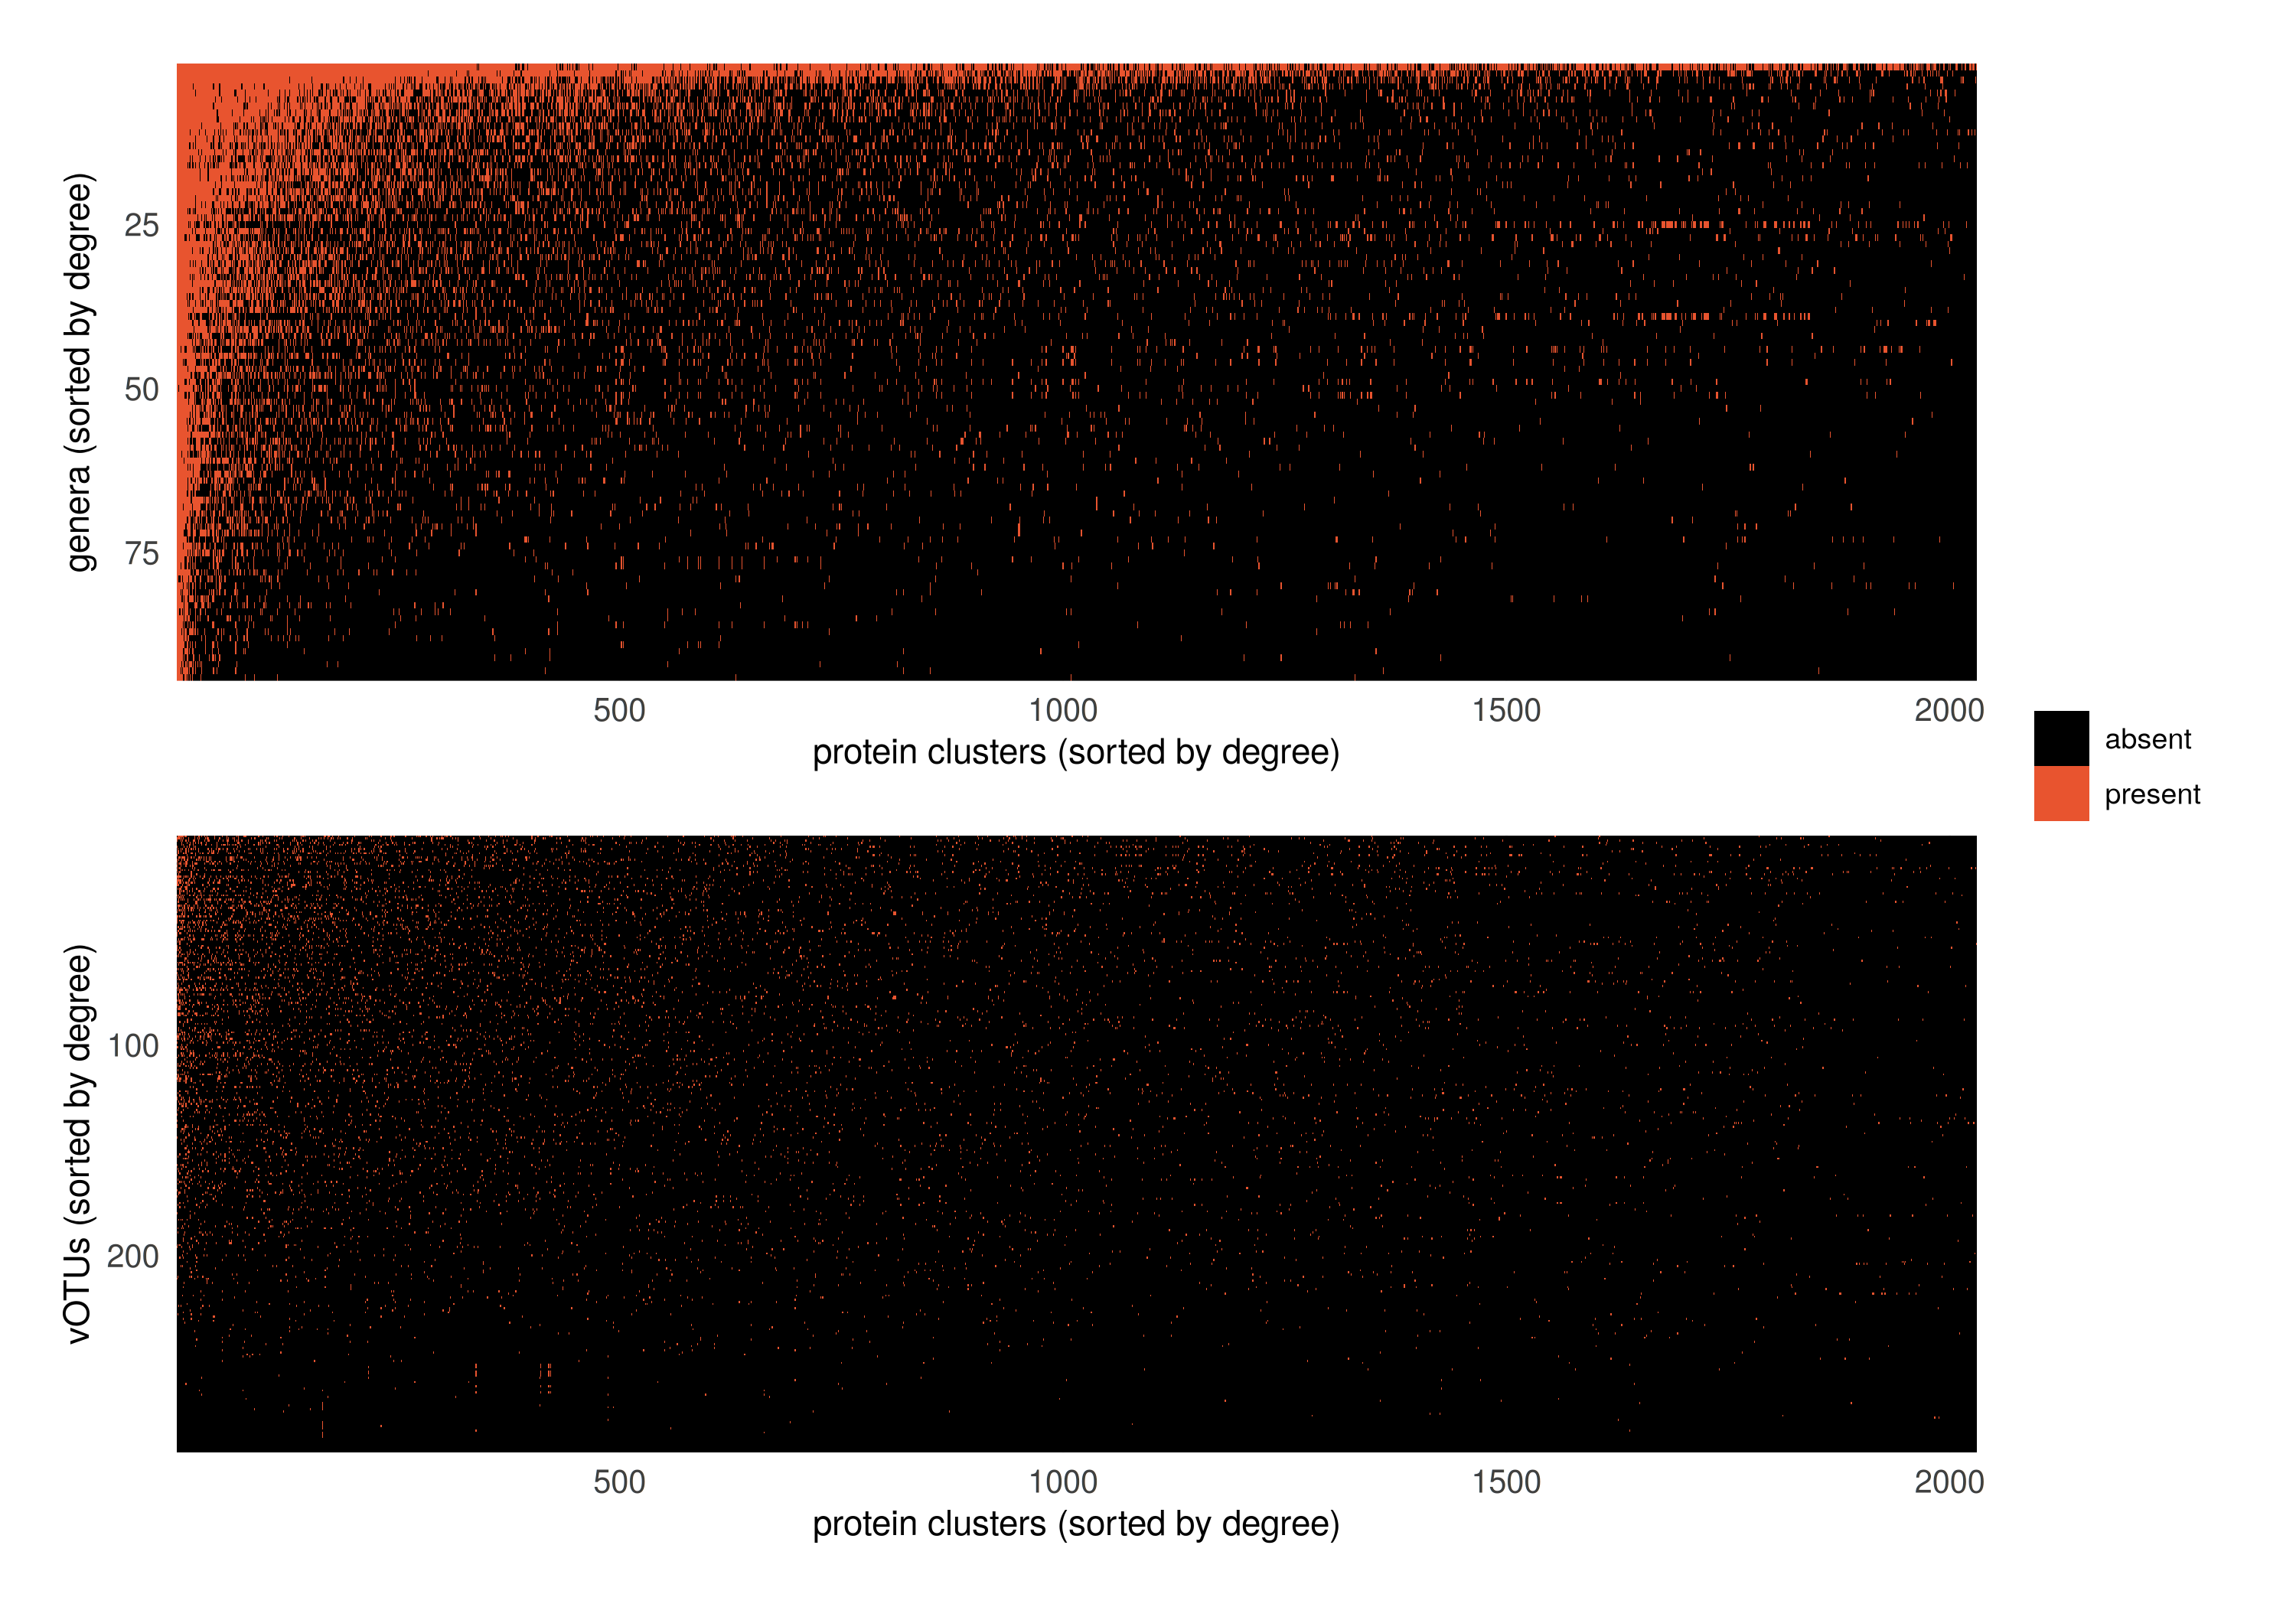
\includegraphics[width=0.88\textwidth]{figures/fig_procsparsity_ibd.png}
  \caption{Protein-cluster sparsity, IBD}
  \label{fig:procsparsity-ibd}
\end{figure}
\FloatBarrier

\begin{figure}[htbp]
  \centering
  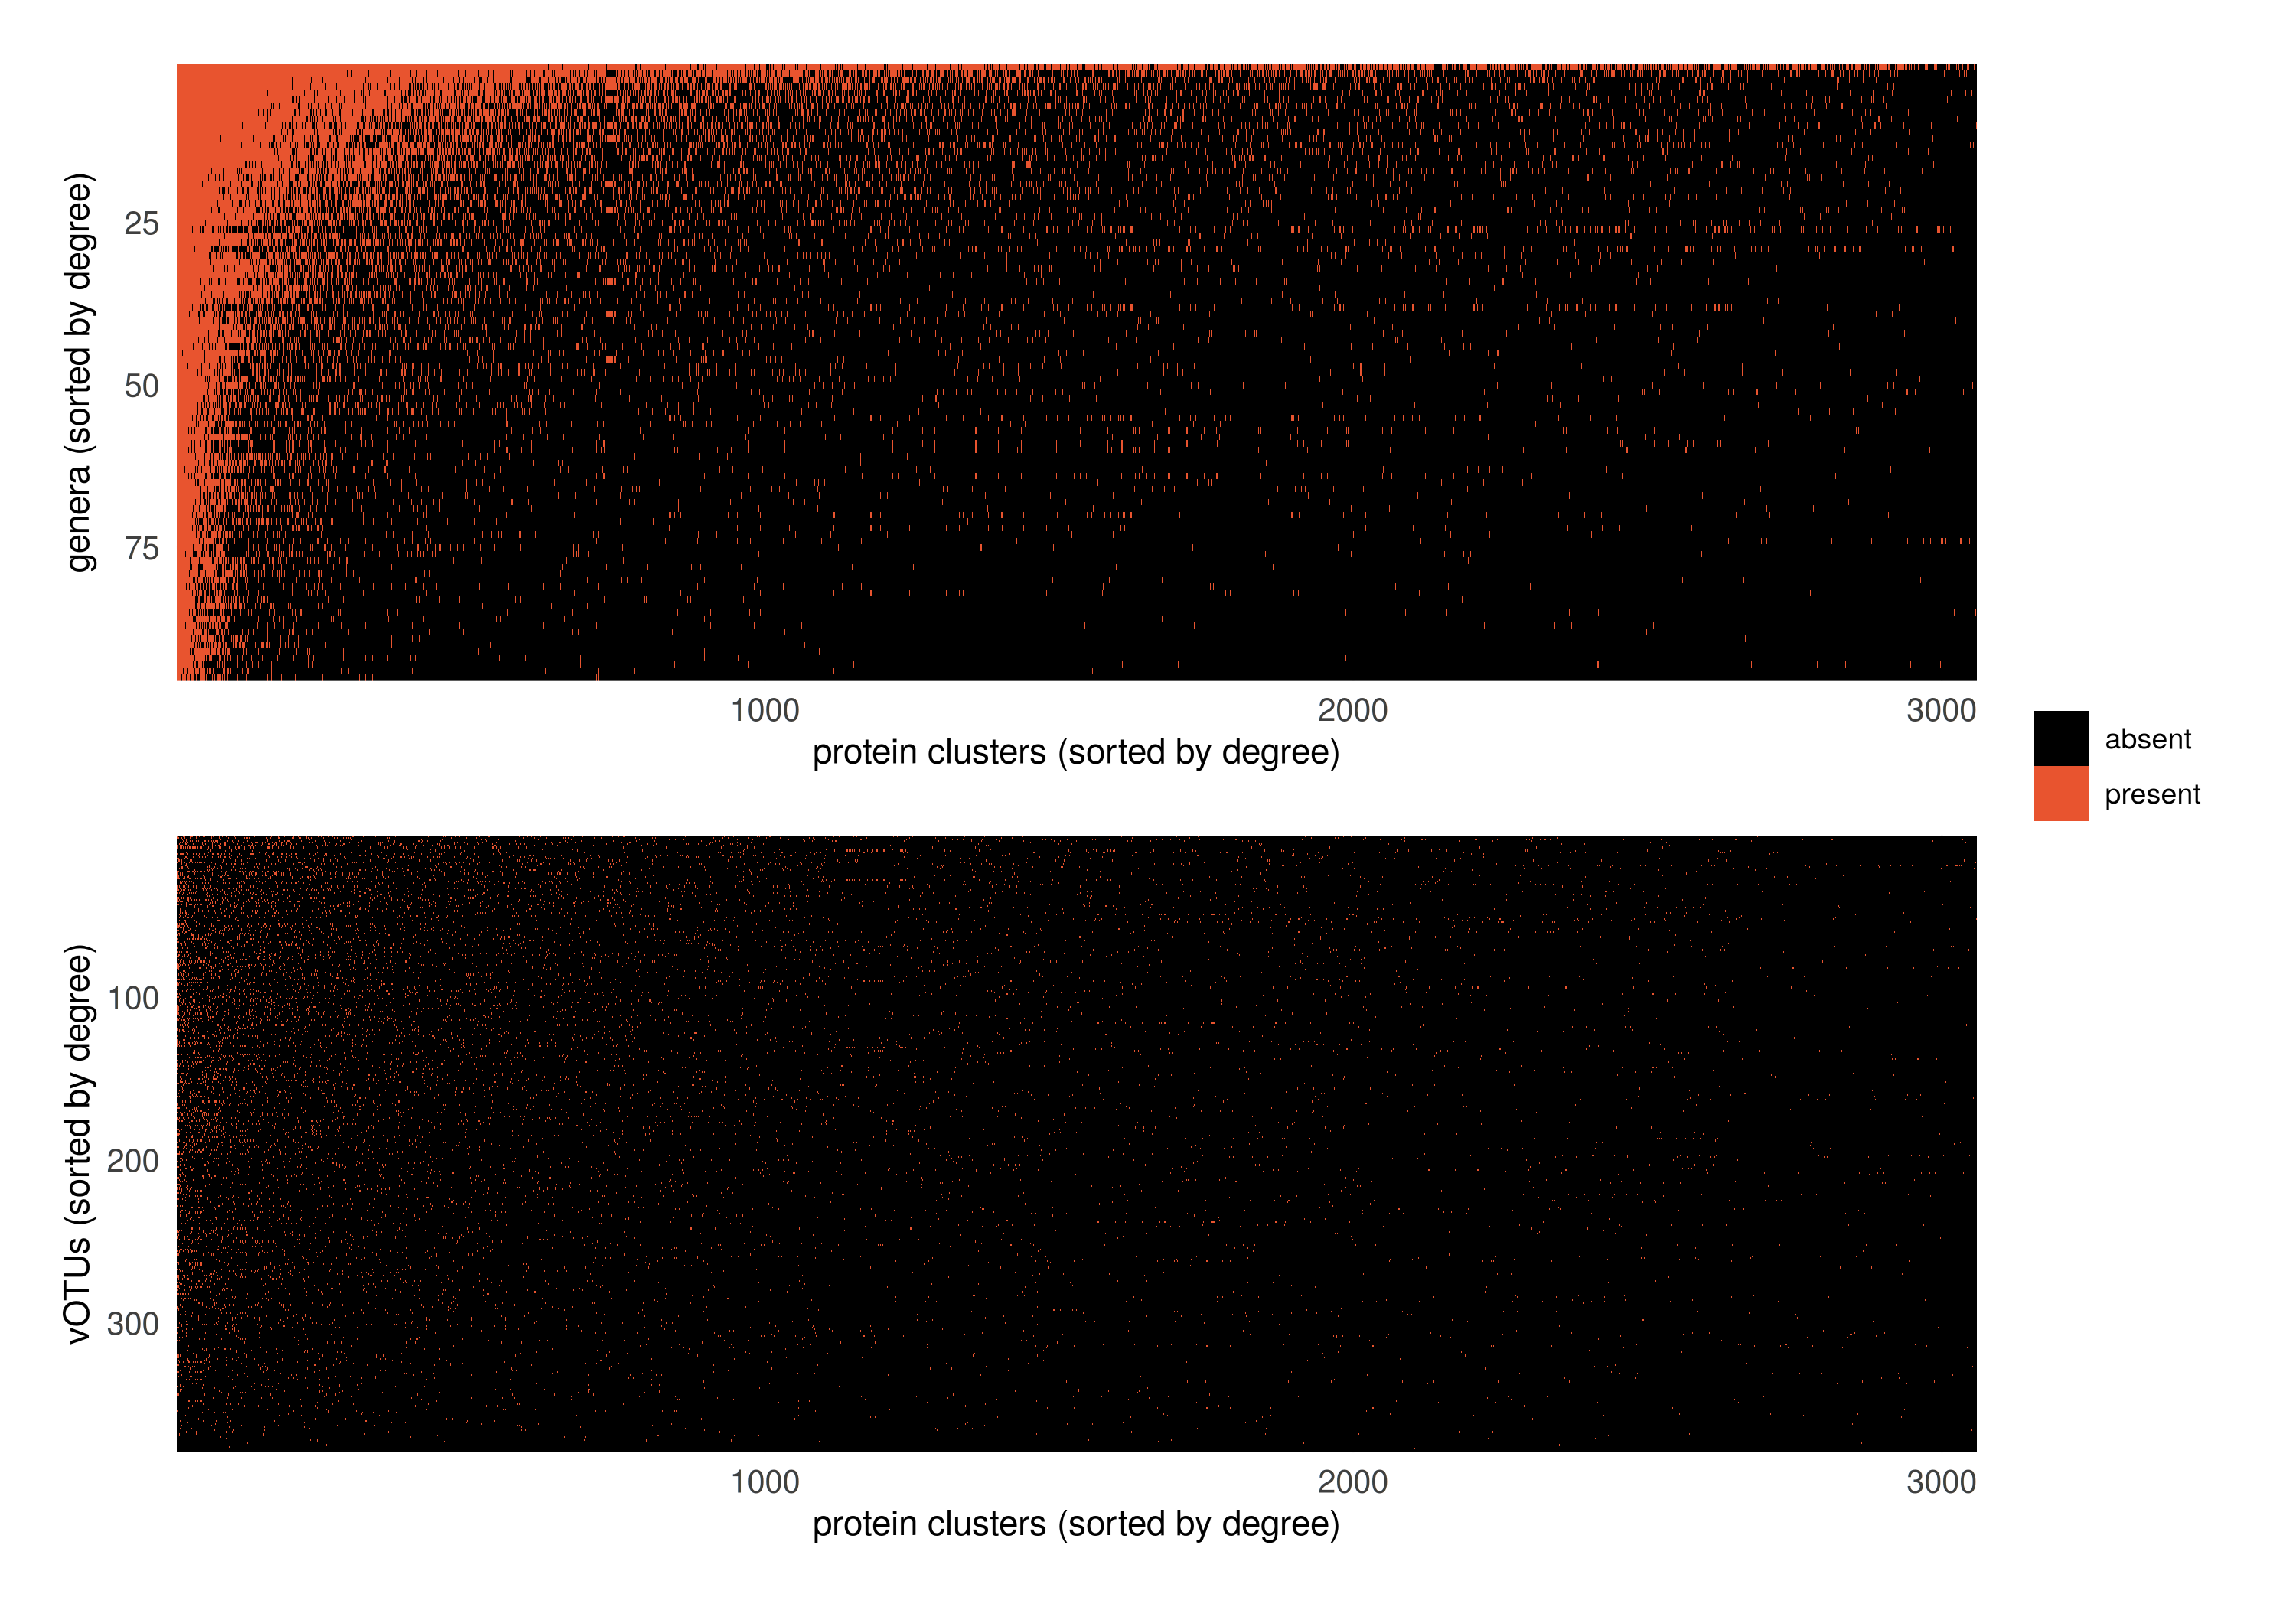
\includegraphics[width=0.88\textwidth]{figures/fig_procsparsity_gvhd.png}
  \caption{Protein-cluster sparsity, GvHD}
  \label{fig:procsparsity-gvhd}
\end{figure}
\FloatBarrier

\subsection{Observed Set of Networks}
\label{res:networks}
Requiring both a protein profile and a CRISPR entry reduces each cohort to the \(n\) bacterial genera and
\(m\) vOTUs that carry both, and the candidate pairs are the \(nm\) combinations of the two. Of the
1{,}360 vOTUs in the CRC viral taxonomy, 573 carry a protein profile and 186 remain once a CRISPR entry
is also required.

The abundance network covers only part of the candidate pairs. In CRC 62 genera and 93 vOTUs are matched,
so the observed set spans 41\% of them; the corresponding figures are $75 \times 70$ (19\%) in IBD and
$56 \times 344$ (54\%) in GvHD. Restricting to the observed pairs barely shifts the CRISPR prevalence,
3.4\% against 3.1\% over all candidate pairs. Table~\ref{tab:descriptives} gives the reduction and both
networks on the observed set.

\begin{table}[htbp]
  \centering
  \caption{Candidate pairs, observed pairs and the two networks, by cohort}
  \label{tab:descriptives}
  \begin{tabular}{lrrr}
    \hline
                              &    CRC &    IBD &   GvHD \\
    \hline
    Samples                   &     84 &    148 &     90 \\
    Bacterial genera kept     &     75 &     94 &     95 \\
    vOTUs kept                &    186 &    293 &    379 \\
    Candidate pairs           & 13,950 & 27,542 & 36,005 \\
    \hline
    Observed pairs            &  5,766 &  5,250 & 19,264 \\
    CRISPR positive           & 198 (3.4\%) & 182 (3.5\%) & 478 (2.5\%) \\
    Selected at least once ($W_{ij}>0$)     & 2,473 (42.9\%) & 2,019 (38.5\%) & 9,451 (49.1\%) \\
    Mean selection probability   &  0.083 &  0.097 &  0.101 \\
    Both                      &     84 &     92 &    265 \\
    \hline
  \end{tabular}
\end{table}
\FloatBarrier

The last row asks whether the two networks mark the same pairs. If they were unrelated, the pairs the
abundance network selects would fall on the observed set without regard to which pairs carry CRISPR
evidence. The overlap is then the number of CRISPR-positive pairs among \(n_W\) draws taken without
replacement from the \(n_{\mathrm{obs}}\) observed pairs, which is hypergeometric. Writing \(n_Y\) and
\(n_W\) for the number of positives of each network,
%
\begin{equation}
  \label{eq:expected-overlap}
  \mathbb{E}[\,\text{both}\,]=\frac{n_Y\,n_W}{n_{\mathrm{obs}}},
  \qquad
  \operatorname{Var}[\,\text{both}\,]
  =n_W\,\frac{n_Y}{n_{\mathrm{obs}}}
   \Bigl(1-\frac{n_Y}{n_{\mathrm{obs}}}\Bigr)
   \frac{n_{\mathrm{obs}}-n_W}{n_{\mathrm{obs}}-1}.
\end{equation}
%
The expected overlap is 85 in CRC, 70 in IBD and 235 in GvHD, against 84, 92 and 265 observed, with
standard deviations of 6.8, 6.4 and 10.8. The observed count is therefore 0.1 standard deviations below
expectation in CRC and 3.4 and 2.8 above it in IBD and GvHD: the two networks mark the same pairs more
often than chance would give in IBD and GvHD, but not in CRC.

In CRC the edge selection probability has a mean of 0.083 and a standard deviation of 0.182, 57\% of the observed
cells are exactly zero and 5\% exceed 0.5. The corresponding shares are 62\% and 7.5\%
in IBD and 51\% and 7.0\% in GvHD.

Over all candidate pairs the median genus carries two to three CRISPR matches and the most connected genus carries 54 in
CRC, 124 in IBD and 156 in GvHD. In every cohort the ten most connected genera account for about 60\% of all
CRISPR edges. The median vOTU carries two matches, with a maximum between 8 and 12.
Figures~\ref{fig:combined-crc} to~\ref{fig:combined-gvhd} show both networks on the observed set: the
edge selection probability as the field and the CRISPR edges outlined on top. Rows and columns are
clustered on \(W\), so the block structure is a property of that ordering.

\begin{figure}[htbp]
  \centering
  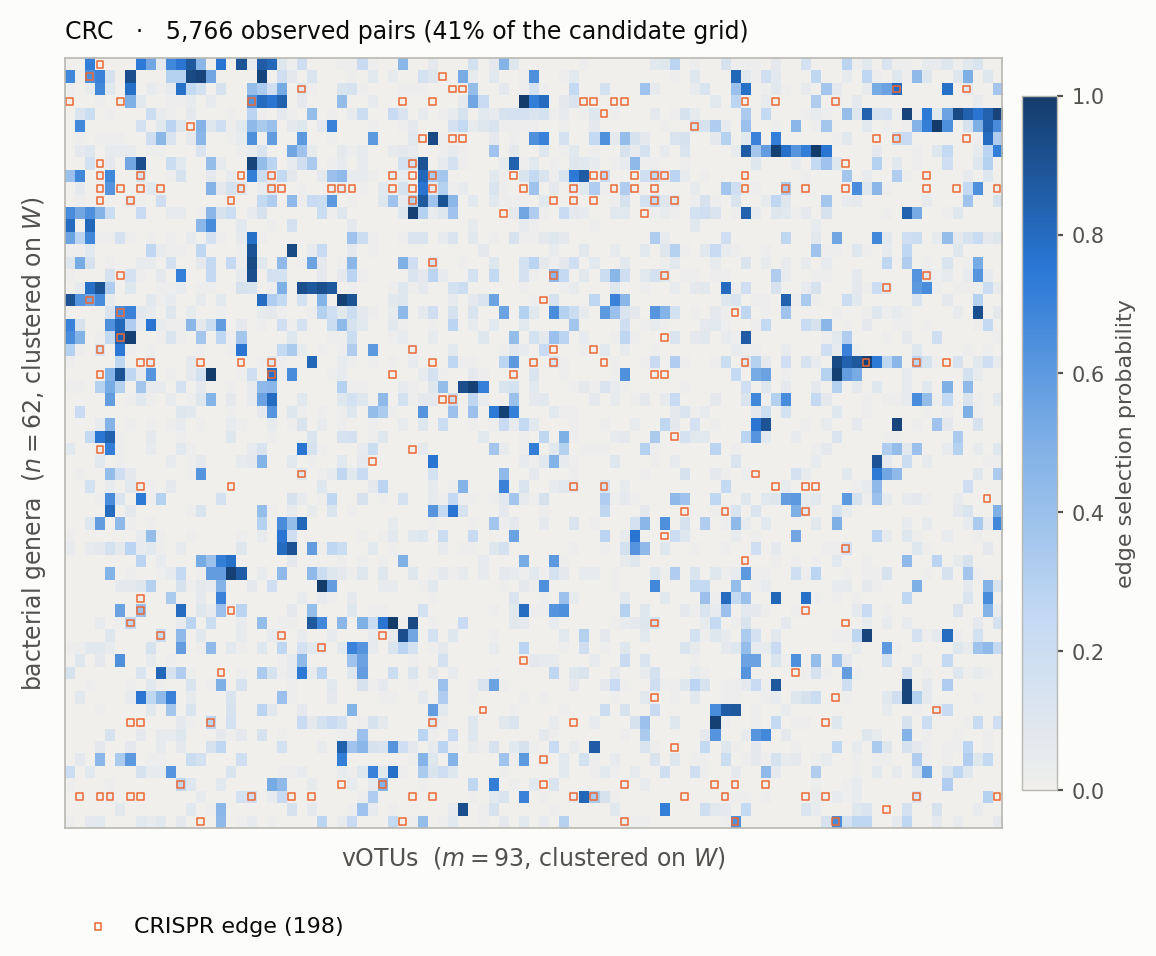
\includegraphics[width=0.80\textwidth]{figures/fig_combined_crc.png}
  \caption{Both networks on the observed set, CRC. Field: edge selection probability. Orange outline: CRISPR edge}
  \label{fig:combined-crc}
\end{figure}
\FloatBarrier

\begin{figure}[htbp]
  \centering
  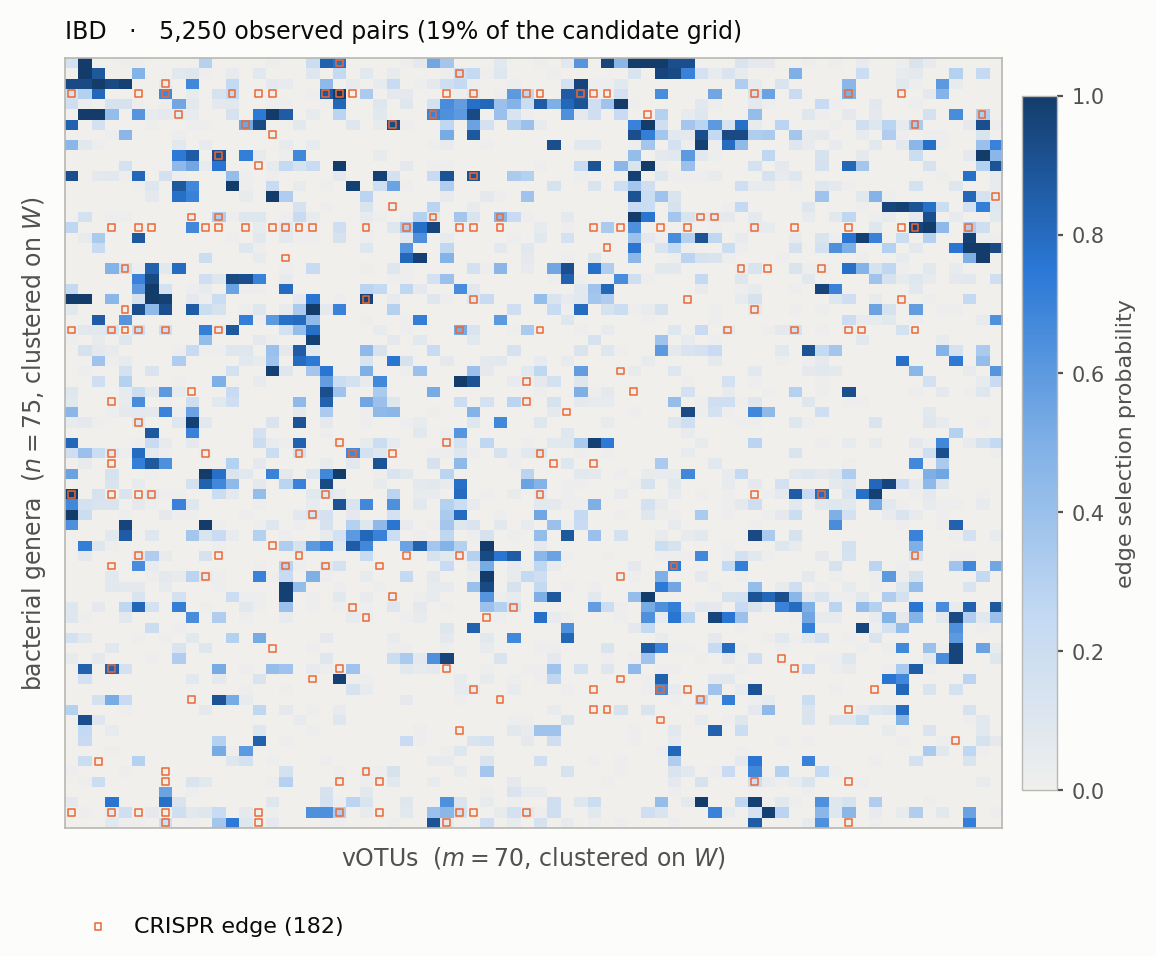
\includegraphics[width=0.80\textwidth]{figures/fig_combined_ibd.png}
  \caption{Both networks on the observed set, IBD. Field: edge selection probability. Orange outline: CRISPR edge}
  \label{fig:combined-ibd}
\end{figure}
\FloatBarrier

\begin{figure}[htbp]
  \centering
  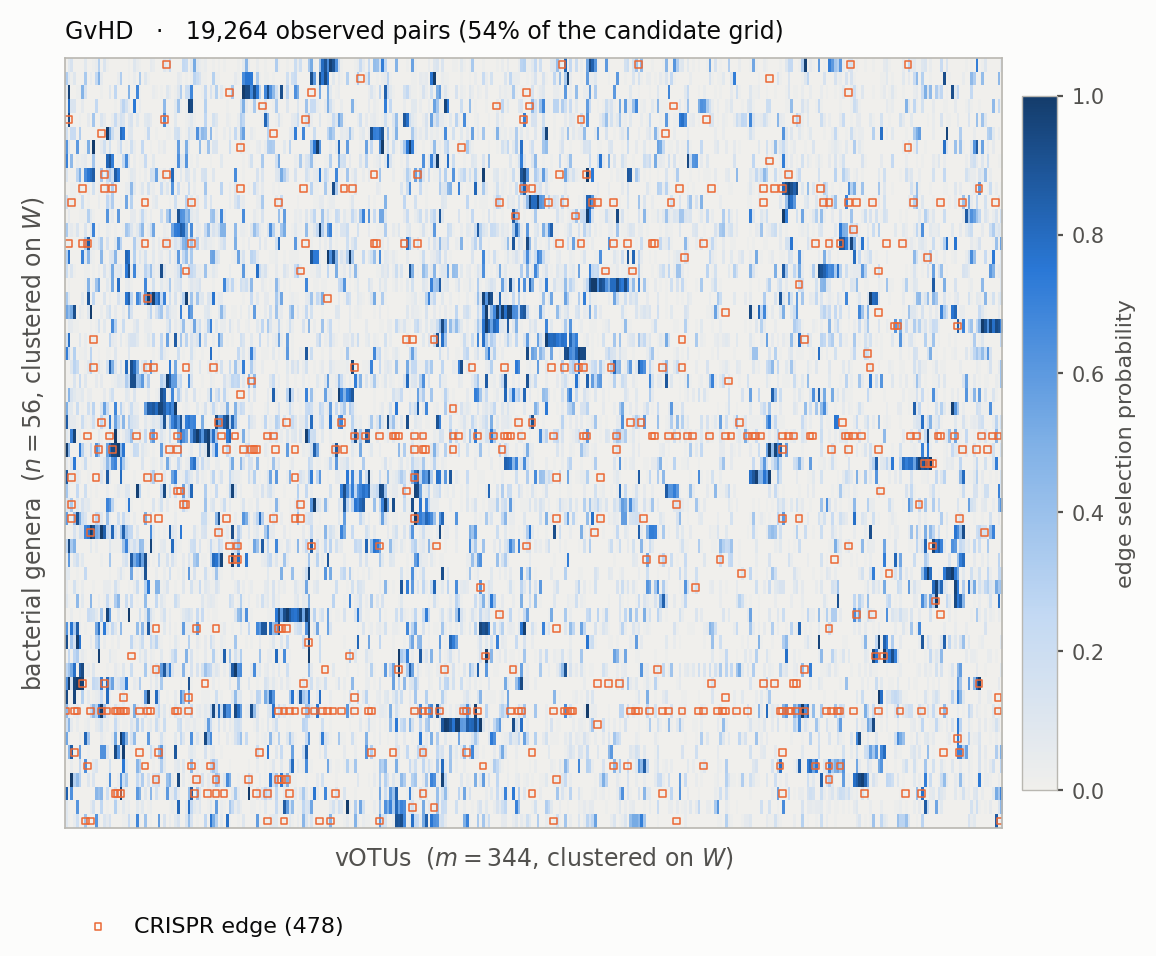
\includegraphics[width=0.80\textwidth]{figures/fig_combined_gvhd.png}
  \caption{Both networks on the observed set, GvHD. Field: edge selection probability. Orange outline: CRISPR edge}
  \label{fig:combined-gvhd}
\end{figure}
\FloatBarrier

\subsection{Prediction Performance}
\label{res:main}

\subsubsection{CRISPR Linkage}
\label{res:main-y}

\begin{table}[htbp]
  \centering
  \caption{Test performance on CRISPR linkage}
  \label{tab:perf-y}
  \begin{tabular}{llrr}
    \hline
    Cohort & Model                     & AUC   & AP    \\
    \hline
    CRC    & Sparse logistic           & 0.758 & 0.185 \\
           & XGBoost                   & 0.788 & 0.213 \\
           & MLP (baseline)            & 0.777 & 0.225 \\
           & MLP (joint)               & 0.775 & 0.253 \\
    \hline
    IBD    & Sparse logistic           & 0.780 & 0.260 \\
           & XGBoost                   & 0.786 & 0.286 \\
           & MLP (baseline)            & 0.740 & 0.269 \\
           & MLP (joint)               & 0.747 & 0.257 \\
    \hline
    GvHD   & Sparse logistic           & 0.767 & 0.129 \\
           & XGBoost                   & 0.798 & 0.186 \\
           & MLP (baseline)            & 0.782 & 0.189 \\
           & MLP (joint)               & 0.780 & 0.200 \\
    \hline
  \end{tabular}
\end{table}

The baseline MLP exceeds sparse logistic on AUC by 0.018 in CRC and 0.015 in GvHD, and is 0.040 below it
in IBD. On AP the difference is $+0.040$ in CRC, $+0.008$ in IBD and $+0.060$ in GvHD.

Against XGBoost the MLP is 0.011 lower in CRC, 0.045 lower in IBD and 0.016 lower in GvHD, whereas on AP
the differences are $+0.012$, $-0.018$ and $+0.003$.

The joint model differs from the baseline MLP on CRISPR AUC by $-0.001$ in CRC, $+0.007$ in IBD and
$-0.001$ in GvHD, with neither model ahead in more than seven of the ten folds. On AP it is 0.028 higher
in CRC, in nine of the ten folds, 0.012 lower in IBD and 0.010 higher in GvHD. The two metrics
therefore disagree in CRC, where sharing a representation leaves the ranking of all pairs unchanged but
improves precision among the highest-scoring ones. At a positive rate of 3.4\% the second is the more
informative comparison, so the joint model is not merely matching the baseline there.

\FloatBarrier

\subsubsection{Edge Selection Probability}
\label{res:main-wreg}

\begin{table}[H]
  \centering
  \caption{Test $R^2$ on the edge selection probability}
  \label{tab:perf-wreg}
  \begin{tabular}{llr}
    \hline
    Cohort & Model              & $R^2$   \\
    \hline
    CRC    & Ridge regression   & $-0.156$ \\
           & XGBoost            & $-0.155$ \\
           & MLP                & $-0.140$ \\
    \hline
    IBD    & Ridge regression   & $-0.153$ \\
           & XGBoost            & $-0.161$ \\
           & MLP                & $-0.130$ \\
    \hline
    GvHD   & Ridge regression   & $-0.172$ \\
           & XGBoost            & $-0.179$ \\
           & MLP                & $-0.143$ \\
    \hline
  \end{tabular}
\end{table}

$R^2$ is negative for every model in every cohort, ranging from $-0.130$ to $-0.179$, and no individual fold of
any model reaches zero.

\subsubsection{Binarised Selection Probability}
\label{res:main-wclass}

\begin{table}[htbp]
  \centering
  \caption{Test performance on the binarised selection probability}
  \label{tab:perf-wclass}
  \begin{tabular}{llrr}
    \hline
    Cohort & Model                     & AUC   & AP    \\
    \hline
    CRC    & Sparse logistic           & 0.590 & 0.498 \\
           & XGBoost                   & 0.579 & 0.495 \\
           & MLP (baseline)            & 0.567 & 0.485 \\
           & MLP (joint)               & 0.586 & 0.501 \\
    \hline
    IBD    & Sparse logistic           & 0.578 & 0.442 \\
           & XGBoost                   & 0.578 & 0.455 \\
           & MLP (baseline)            & 0.606 & 0.480 \\
           & MLP (joint)               & 0.605 & 0.480 \\
    \hline
    GvHD   & Sparse logistic           & 0.599 & 0.582 \\
           & XGBoost                   & 0.590 & 0.568 \\
           & MLP (baseline)            & 0.590 & 0.570 \\
           & MLP (joint)               & 0.603 & 0.586 \\
    \hline
  \end{tabular}
\end{table}

Every model in every cohort sits between 0.567 and 0.606 AUC. The baseline MLP is 0.023 below sparse
logistic in CRC, 0.028 above it in IBD and 0.008 below it in GvHD; on AP the differences are $-0.013$,
$+0.038$ and $-0.012$. XGBoost is 0.011 below sparse logistic in CRC, level with it in IBD and 0.009 below
in GvHD.

The joint model exceeds the baseline MLP by 0.020 in CRC and 0.013 in GvHD, in nine and eight of the ten
folds, with a difference of $-0.001$ in IBD. Against sparse logistic it is 0.004 lower in CRC, 0.027
higher in IBD and 0.004 higher in GvHD.

\FloatBarrier

\subsection{Representation Comparison}
\label{res:cka}
We compute all values below on latent coordinates scaled to unit variance and report them as a mean and
standard deviation over the ten held-out folds.

The two single-head layers are the least aligned pair in every cohort, at 0.264 (0.010) in CRC,
0.134 (0.019) in IBD and 0.093 (0.024) in GvHD. The shared layer of the joint model is far closer to the
layer fitted to \(Y\), at 0.768 (0.016), 0.565 (0.049) and 0.847 (0.041), than to the layer fitted to the
binarised edge weight, at 0.345 (0.019), 0.386 (0.015) and 0.167 (0.024).

The alignment of the shared layer with the layer fitted to the binarised edge weight nevertheless
exceeds that between the two single-head layers in all three cohorts, by 0.081 in CRC, 0.251 in IBD
and 0.073 in GvHD.

Fold-to-fold variation is small, between 0.010 and 0.024 for seven of the nine values; the exceptions are
the alignment with \(H^{Y}\) in IBD (0.049) and in GvHD (0.041).
Figures~\ref{fig:cka-crc} to~\ref{fig:cka-gvhd} show the three pairwise values per cohort.

\begin{figure}[htbp]
  \centering
  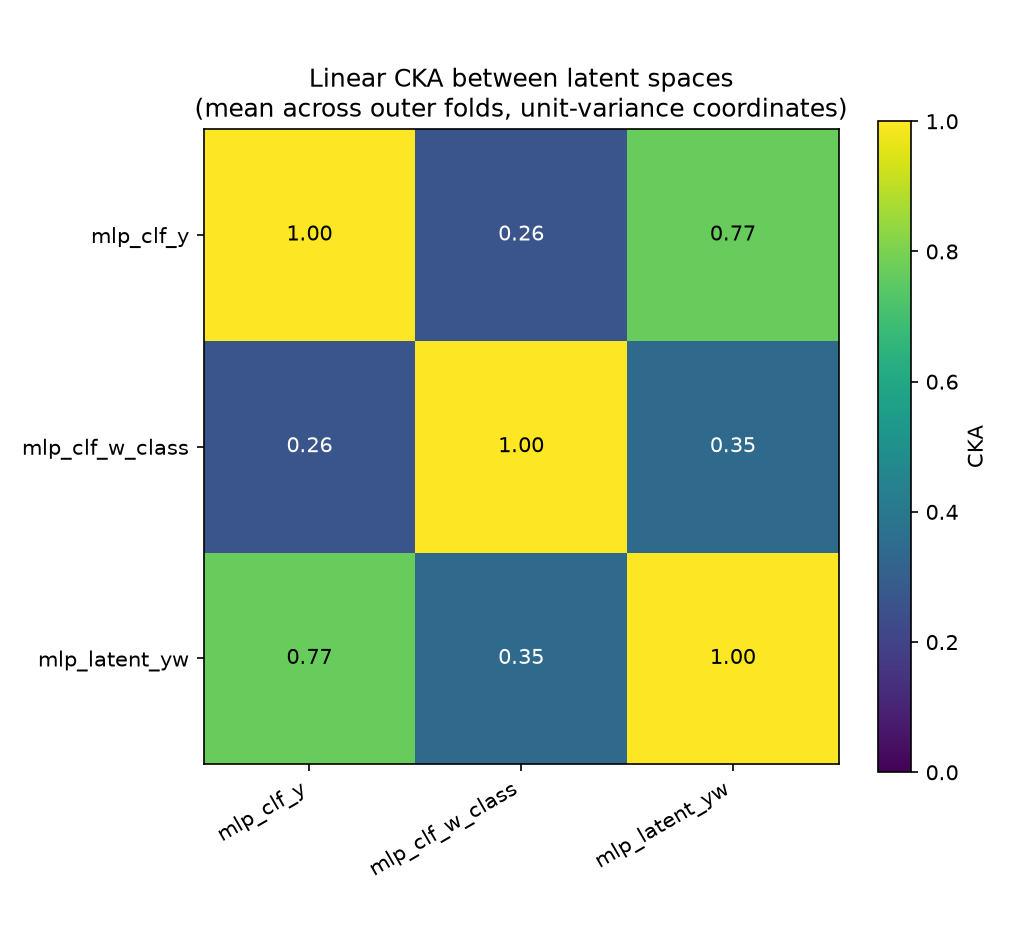
\includegraphics[width=0.60\textwidth]{figures/fig_cka_crc.png}
  \caption{Linear CKA between the fitted hidden layers on unit-variance coordinates, mean over the ten
  held-out folds, CRC}
  \label{fig:cka-crc}
\end{figure}
\FloatBarrier

\begin{figure}[htbp]
  \centering
  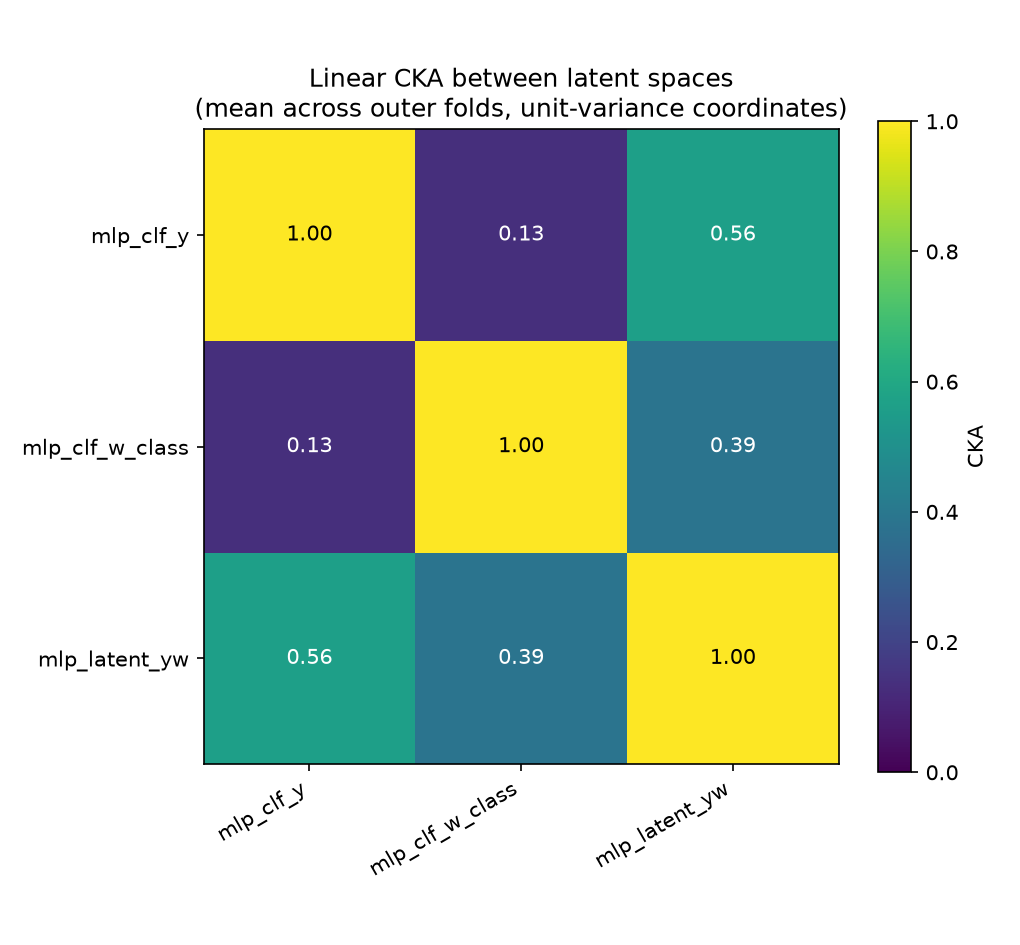
\includegraphics[width=0.60\textwidth]{figures/fig_cka_ibd.png}
  \caption{Linear CKA between the fitted hidden layers on unit-variance coordinates, mean over the ten
  held-out folds, IBD}
  \label{fig:cka-ibd}
\end{figure}
\FloatBarrier

\begin{figure}[htbp]
  \centering
  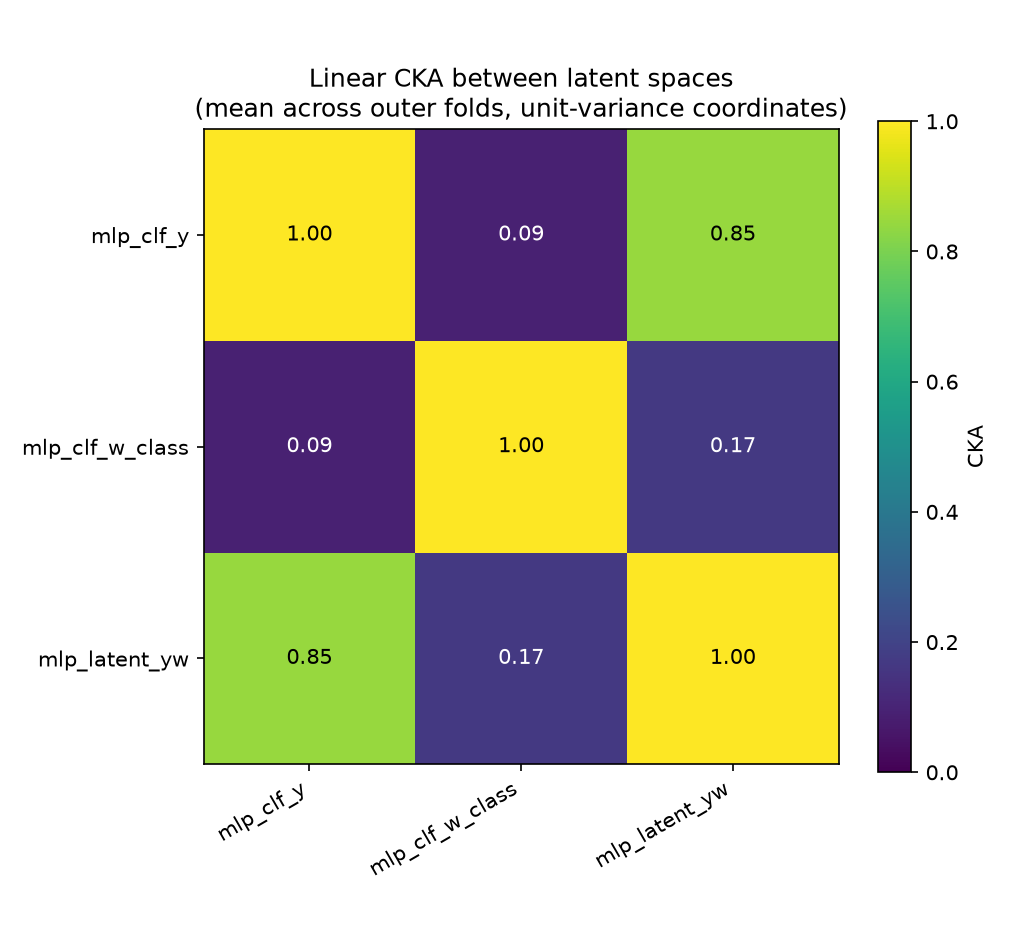
\includegraphics[width=0.60\textwidth]{figures/fig_cka_gvhd.png}
  \caption{Linear CKA between the fitted hidden layers on unit-variance coordinates, mean over the ten
  held-out folds, GvHD}
  \label{fig:cka-gvhd}
\end{figure}
\FloatBarrier

\subsection{Shuffled-CRISPR Control}
\label{res:joint}

\begin{table}[htbp]
  \centering
  \caption{Shuffled-CRISPR control: real vs permuted CRISPR labels}
  \label{tab:shuffle-y}
  \begin{tabular}{lllrr}
    \hline
    Cohort & Head               & CRISPR labels & AUC   & AP    \\
    \hline
    CRC    & CRISPR             & Real       & 0.775 & 0.253 \\
           &                    & Permuted   & 0.476 & 0.042 \\
           & edge selection probability        & Real       & 0.586 & 0.501 \\
           &                    & Permuted   & 0.580 & 0.496 \\
    \hline
    IBD    & CRISPR             & Real       & 0.747 & 0.257 \\
           &                    & Permuted   & 0.487 & 0.050 \\
           & edge selection probability        & Real       & 0.605 & 0.480 \\
           &                    & Permuted   & 0.599 & 0.475 \\
    \hline
    GvHD   & CRISPR             & Real       & 0.780 & 0.200 \\
           &                    & Permuted   & 0.508 & 0.031 \\
           & edge selection probability        & Real       & 0.603 & 0.586 \\
           &                    & Permuted   & 0.602 & 0.587 \\
    \hline
  \end{tabular}
\end{table}

On the CRISPR head the permutation moves AUC from 0.747--0.780 to 0.476--0.508 and AP from 0.200--0.257
to 0.031--0.050, in every fold of every cohort.

On the association head the difference between real and permuted CRISPR labels is $+0.007$ in CRC,
$+0.005$ in IBD and $+0.001$ in GvHD, with the real labels ahead on AUC in eight, seven and six of the ten
folds. The permuted joint model reaches 0.580 on the edge selection probability against 0.567 for the baseline
 MLP in CRC, 0.599 against 0.606 in IBD and 0.602 against 0.590 in GvHD.

Figures~\ref{fig:shuffle-crc} to~\ref{fig:shuffle-gvhd} give the real and permuted scores per cohort.

\begin{figure}[htbp]
  \centering
  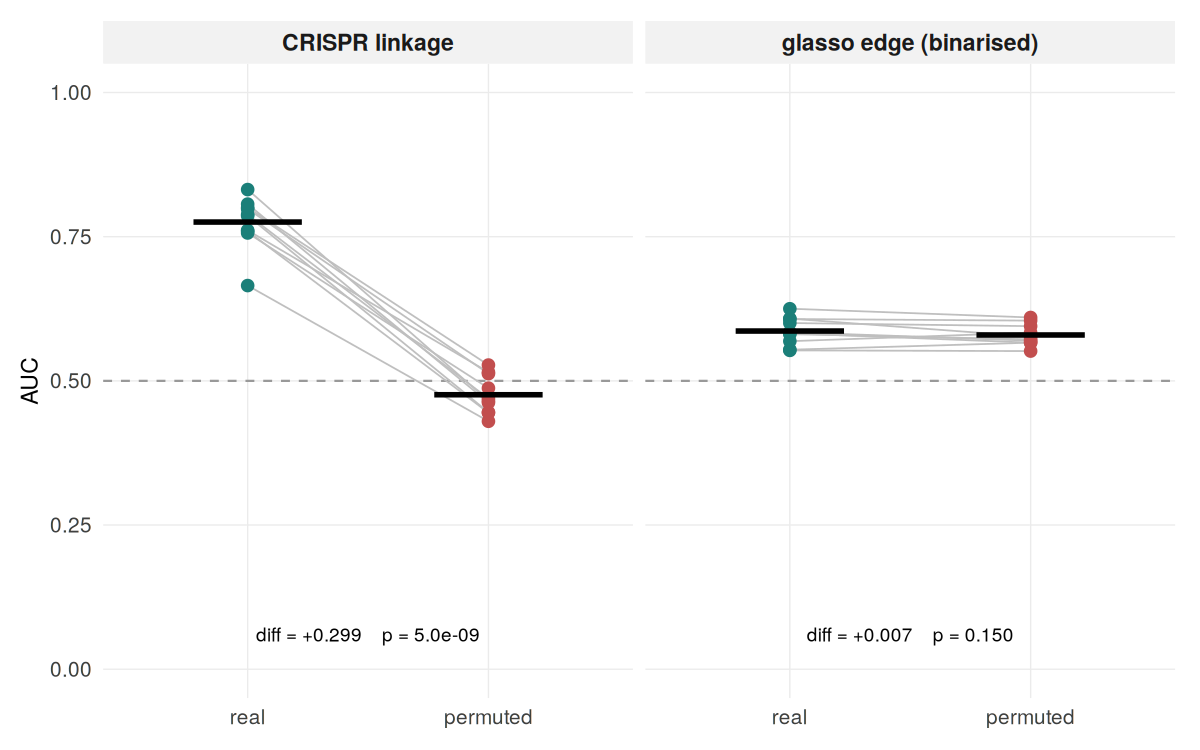
\includegraphics[width=0.88\textwidth]{figures/fig_shuffle_crc.png}
  \caption{Real against permuted CRISPR labels, CRC}
  \label{fig:shuffle-crc}
\end{figure}
\FloatBarrier

\begin{figure}[htbp]
  \centering
  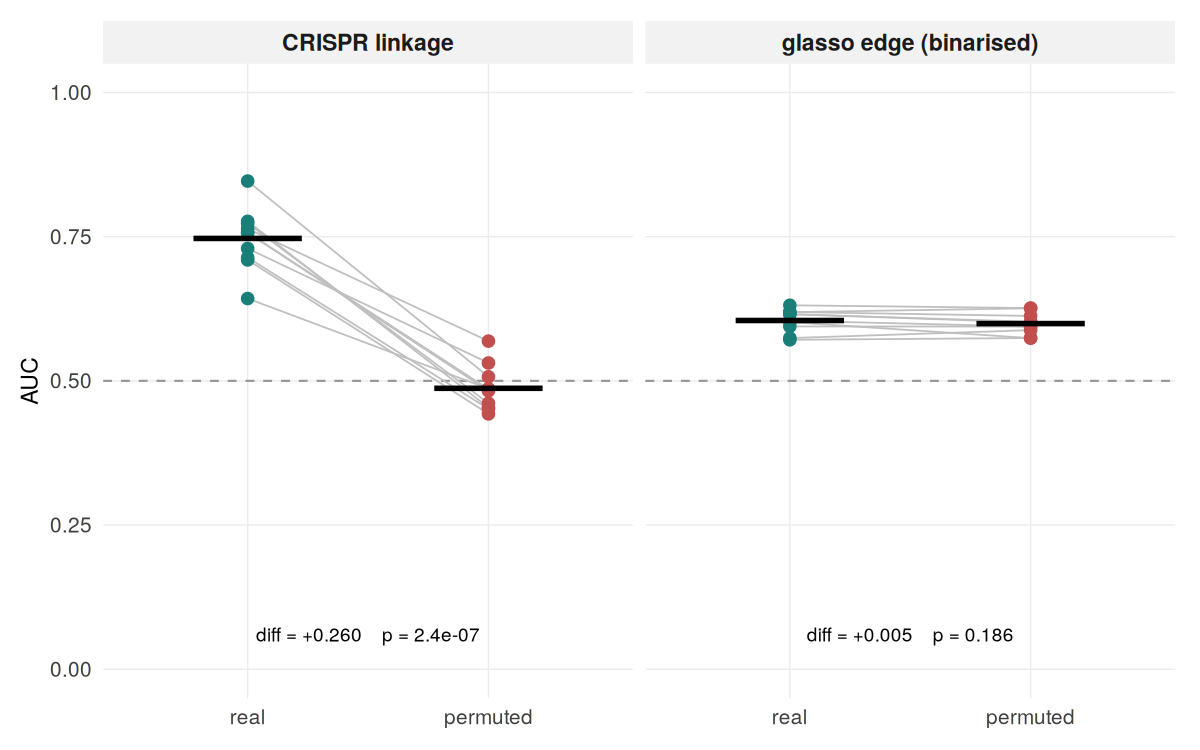
\includegraphics[width=0.88\textwidth]{figures/fig_shuffle_ibd.png}
  \caption{Real against permuted CRISPR labels, IBD}
  \label{fig:shuffle-ibd}
\end{figure}
\FloatBarrier

\begin{figure}[htbp]
  \centering
  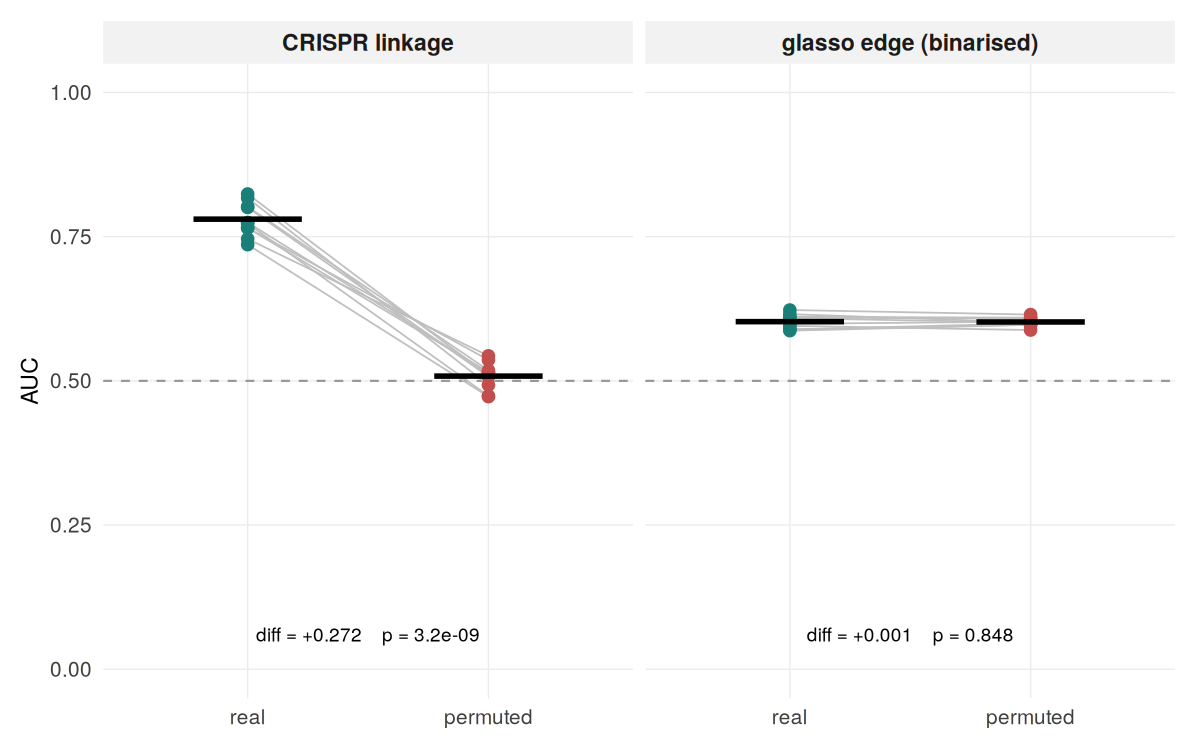
\includegraphics[width=0.88\textwidth]{figures/fig_shuffle_gvhd.png}
  \caption{Real against permuted CRISPR labels, GvHD}
  \label{fig:shuffle-gvhd}
\end{figure}
\FloatBarrier
\subsection{Stability Selection}
\label{res:stability}
Table~\ref{tab:stability} gives the stability selection over the shared protein clusters, run on CRISPR linkage
over the observed pairs with $B = 50$ subsamples at $\pi_{\mathrm{thr}} = 0.8$. The candidate set is 1{,}103
clusters in CRC, 2{,}013 in IBD and 3{,}051 in GvHD, giving $q = 25$, $34$ and $42$. Every resample reached
$q$, with an average support of 27.5, 36.8 and 47.2 clusters, so the bound of
Equation~\eqref{eq:mbbound} evaluated at the realised average support is 1.14, 1.12 and 1.21.

No cluster reaches the threshold in any cohort, and none is selected in half of the resamples. The highest
selection probability is 0.46 in CRC, 0.36 in IBD and 0.30 in GvHD.
Figure~\ref{fig:ap-stab} in the appendix gives the selection probabilities per cohort.

\begin{table}[htbp]
  \centering
  \caption{Stability selection over the shared protein clusters, CRISPR linkage}
  \label{tab:stability}
  \begin{tabular}{lrrrrrr}
    \hline
    Cohort & $n_{\text{obs}}$ & $d$ & $q$ & Mean support & Stable & Max.\ selection prob. \\
    \hline
    CRC  &  5,766 & 1,103 & 25 & 27.5 & 0 & 0.46 \\
    IBD  &  5,250 & 2,013 & 34 & 36.8 & 0 & 0.36 \\
    GvHD & 19,264 & 3,051 & 42 & 47.2 & 0 & 0.30 \\
    \hline
  \end{tabular}
\end{table}
\FloatBarrier


\newpage

\section{Discussion}
\label{discussion}
\subsection{Interpretation of the Main Findings}
The two networks differ greatly in how well they can be predicted from the pair feature \(z_{ij}\).
CRISPR linkage \(Y_{ij}\) is predicted well above chance in all three cohorts, with the nonlinear models
strongest. The edge selection probability is much harder. On its original scale the regression models give
negative \(R^{2}\) in every cohort, so they do not improve on the constant test-fold mean; after
binarisation the AUC rises but remains only moderately above \(0.5\).

Part of the negative \(R^{2}\) follows from how \(W\) is constructed rather than from the features: the
models are fitted on the logit scale and scored on \([0,1]\), and more than half of the observed
\(W_{ij}\) are exactly zero.

The gap between the two networks is stable across the modelling choices examined. Increasing flexibility
from linear to nonlinear models helps \(Y_{ij}\) more than \(W_{ij}\). The pair
feature therefore carries more information about CRISPR linkage than about the edge selection probability.

The joint model matches the separate ones in accuracy, but the representation it learns is not a
compromise between the two networks. Linear CKA between the fitted hidden layers places the shared layer
close to the layer fitted to CRISPR linkage and far from the one fitted to the
binarised edge weight, while the two single-head layers are barely aligned with
each other. One representation therefore suffices for both, but it is
essentially the one CRISPR linkage induces on its own, which the edge weight can also use. One of the reasons for it
may be that CRISPR linkage is rare while the binarised edge weight is near-balanced, so after class
weighting the CRISPR term contributes the larger gradient to the shared layer. The alignment with the
edge-weight layer is nevertheless higher for the shared layer than for the CRISPR layer in all three
cohorts, so the second head does shape the representation, only weakly.

\subsection{Limitations and Future Work}
The cross-validation holds out pairs rather than organisms, so the reported performance describes
generalisation to new pairings of known genera and vOTUs, not to unseen organisms.

Both networks are indirect proxies for infection. Absence of CRISPR evidence does not imply absence of an
interaction, and \(W_{ij}\) records how reproducibly an inferred conditional association is selected
rather than observed infection \citep{coenen2018,pinto2022,alrasheed2019}.

The regression on \(W_{ij}\) is fitted on the logit scale, because \(W_{ij}\) is bounded while the models
predict on the real line. Mapping the fitted values back through the sigmoid does not recover the
conditional mean, since \(\sigma\bigl(\mathbb{E}[\widetilde W_{ij}\mid z_{ij}]\bigr)\neq
\mathbb{E}[W_{ij}\mid z_{ij}]\), so the reported \(R^{2}\) grades a conditional median against a
mean-based criterion. Moreover, with more than half of the observed
\(W_{ij}\) exactly zero, every such pair takes the value \(\operatorname{logit}(\varepsilon)\approx
-6.91\) with clipping, and a different \(\varepsilon\) would move that point mass and with it the fit. 

The models use only pair-level protein information. This is a particular restriction for \(W_{ij}\), which
is estimated from the multivariate structure of the whole community, and genus-level aggregation may
obscure strain-specific host relationships.

The protein cluster vocabularies are built within each cohort and share almost no clusters, so an
individual cluster has no counterpart in the other cohorts. Cross-cohort transfer and any cross-cohort
reading of the selected clusters would require a common vocabulary.

The pair feature also limits what the models can express. A linear model on
\(z_{ij}=\operatorname{bin}(x^{b}_{i})+\operatorname{bin}(x^{v}_{j})\) reduces to a bacterium term plus a
vOTU term, so only the nonlinear models can use the coordinates where both partners carry the cluster,
and those take the value \(2\) in \(0.3\)--\(0.4\%\) of entries on the observed pairs. Adding the coordinatewise product
\(\operatorname{bin}(x^{b}_{i})\odot\operatorname{bin}(x^{v}_{j})\) alongside the two halves would make
that co-occurrence an explicit coordinate rather than a level of a three-valued one.

Future work could evaluate organism-held-out and cross-cohort generalisation, incorporate experimentally
validated host interactions \citep{shang2025}, and build shared protein representations from functional
annotation or protein-sequence embeddings \citep{lin2023}. For \(W_{ij}\), a two-part model separating
whether an edge is ever selected from how often it is selected would match the observed distribution
better than a single regression on the logit scale.

\newpage

\section{Conclusion}
\label{conclusion}
CRISPR linkage is consistently predictable from protein cluster profiles across all three cohorts, while
the edge selection probability remains weakly predictable whether it is treated as continuous or
binarised, and across model classes.

A single shared representation predicts both binary networks without substantial loss on CRISPR linkage.
The small gains it produces for the edge selection probability persist when the CRISPR training labels are
permuted, so they cannot be attributed to information specific to CRISPR linkage and are consistent with
an effect of the joint architecture or the optimisation itself.

Comparing the fitted hidden layers shows what that shared representation is: in every cohort it is close
to the one CRISPR linkage induces on its own and far from the one the edge weight induces. One
representation serves both networks, but it is not a compromise between them.

Stability selection returns no protein cluster above the selection threshold in any cohort, giving no
evidence for a small set of universally predictive clusters.


\newpage

% ------------------------------------------------------------------------------
% APPENDIX ---------------------------------------------------------------------
% ------------------------------------------------------------------------------

\pagenumbering{Roman}

\setcounter{page}{5} % CHANGE

\appendix

\section{Appendix}
\label{app}
Every figure produced by the pipeline that is not reproduced in Section~\ref{results} is collected here,
with the three cohorts side by side. All of them are drawn from the run \texttt{20260916\_152830}.

\subsection{Descriptive Plots}

\begin{figure}[H]
  \centering
  \begin{subfigure}[t]{0.32\textwidth}
    \centering
    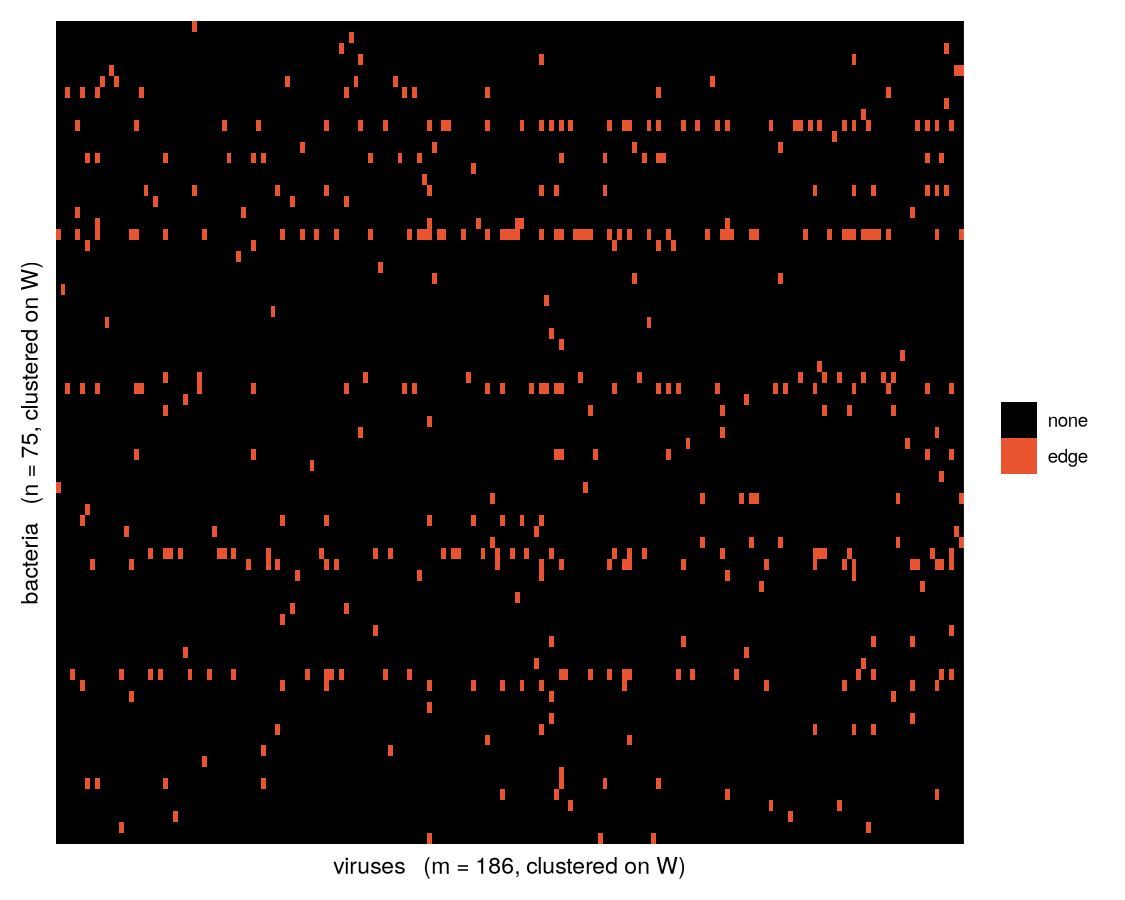
\includegraphics[width=\linewidth]{figures/fig_ap_interaction_Y_matrix_crc.png}
    \caption{CRC}
  \end{subfigure}\hfill
  \begin{subfigure}[t]{0.32\textwidth}
    \centering
    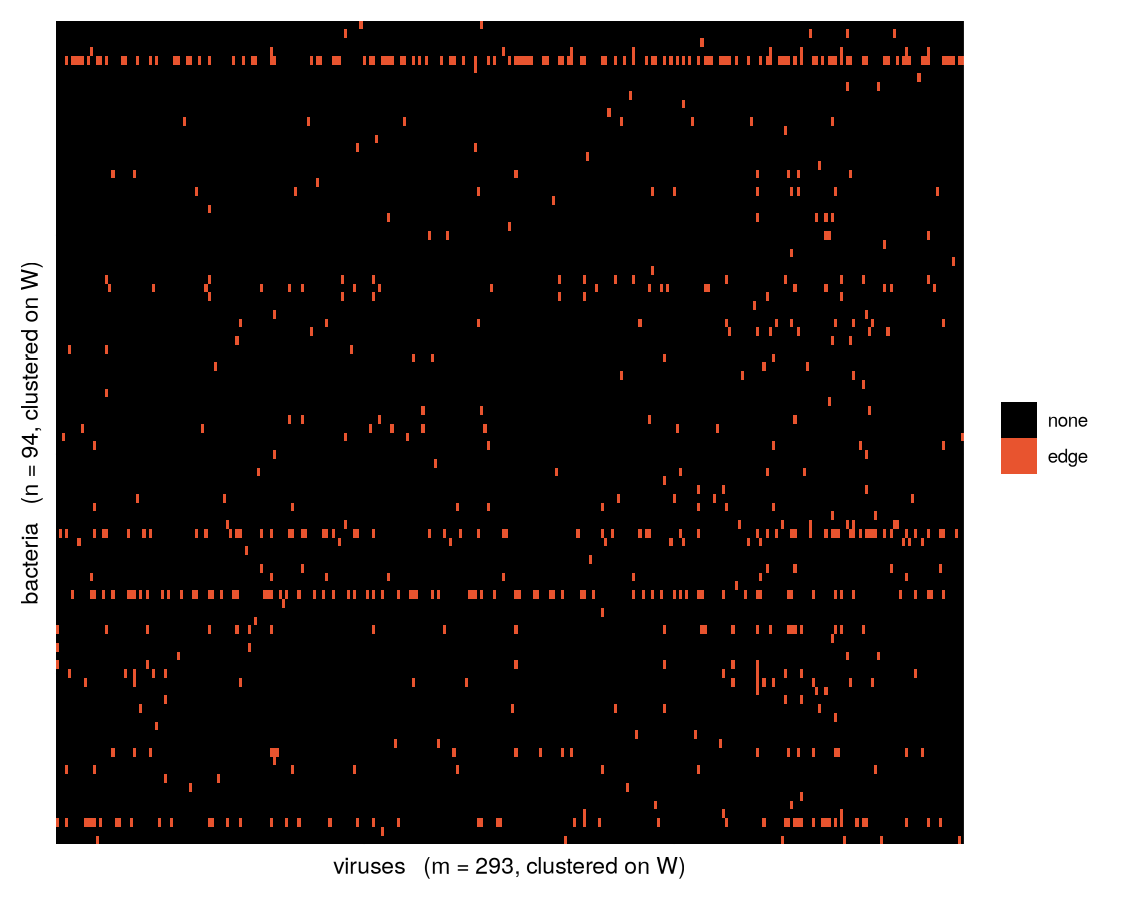
\includegraphics[width=\linewidth]{figures/fig_ap_interaction_Y_matrix_ibd.png}
    \caption{IBD}
  \end{subfigure}\hfill
  \begin{subfigure}[t]{0.32\textwidth}
    \centering
    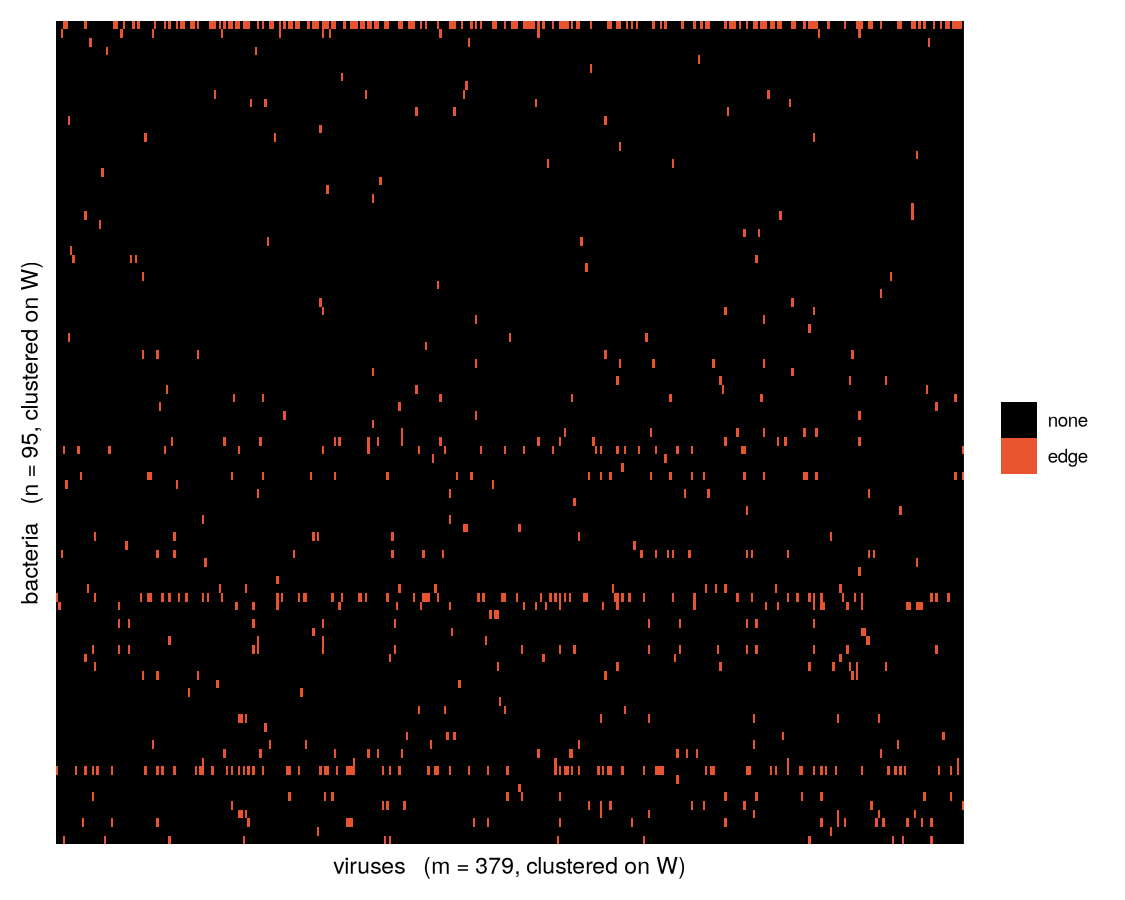
\includegraphics[width=\linewidth]{figures/fig_ap_interaction_Y_matrix_gvhd.png}
    \caption{GvHD}
  \end{subfigure}
  \caption{CRISPR linkage over all candidate pairs}
  \label{fig:ap-ymat}
\end{figure}

\begin{figure}[H]
  \centering
  \begin{subfigure}[t]{0.32\textwidth}
    \centering
    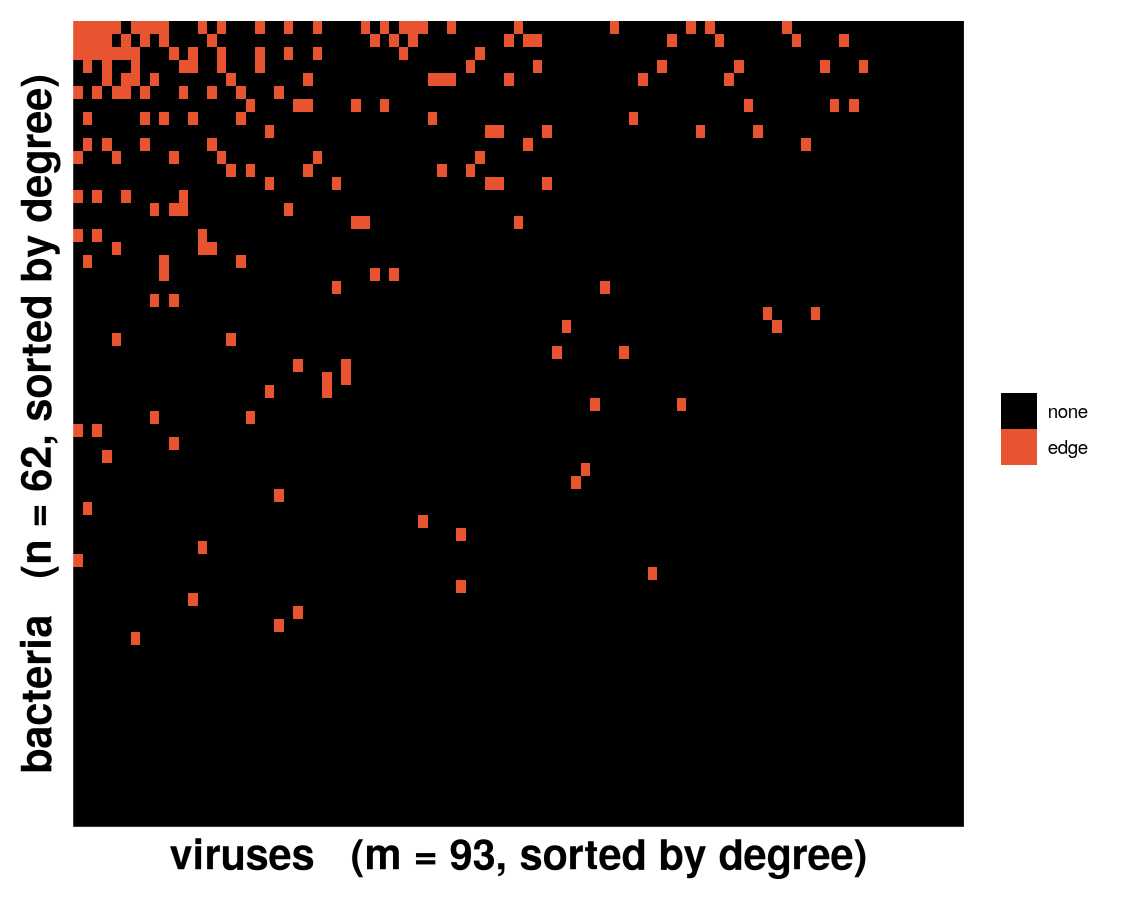
\includegraphics[width=\linewidth]{figures/fig_ap_interaction_Y_matrix_observed_crc.png}
    \caption{CRC}
  \end{subfigure}\hfill
  \begin{subfigure}[t]{0.32\textwidth}
    \centering
    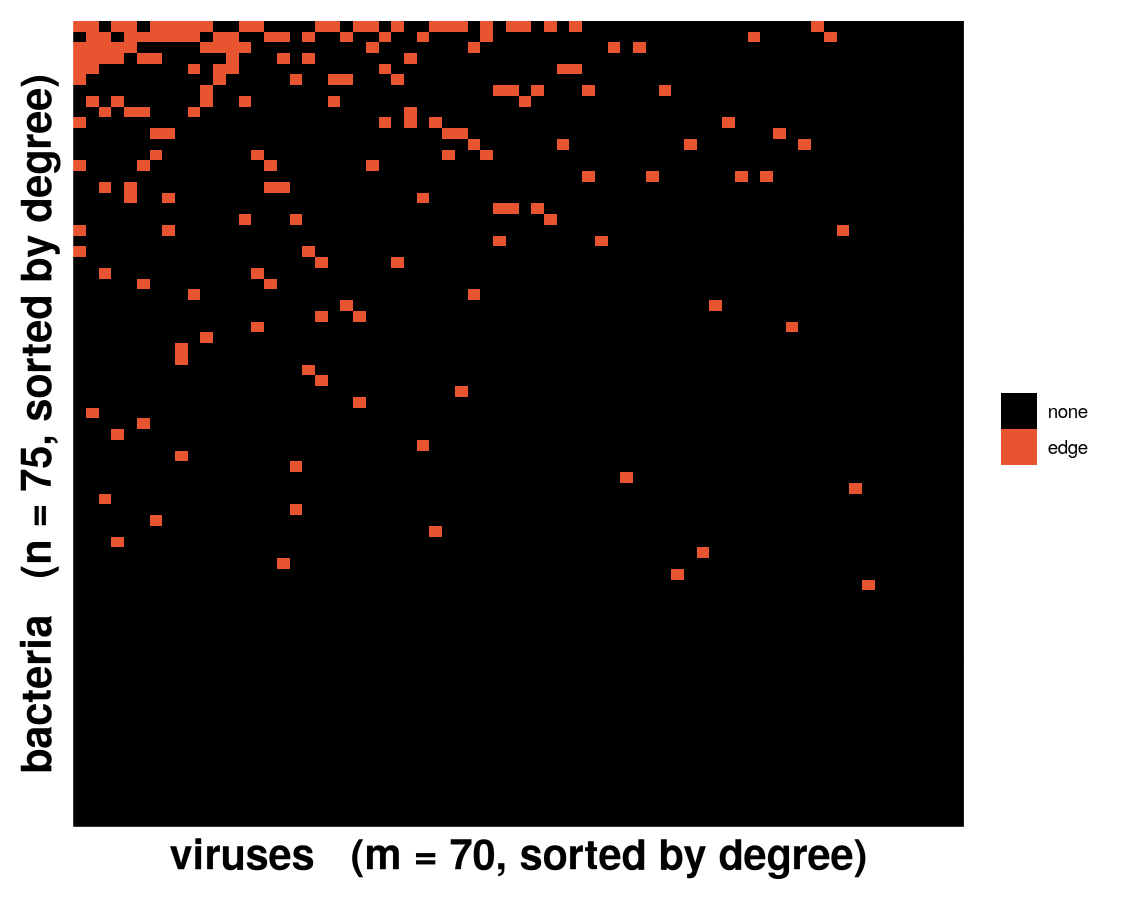
\includegraphics[width=\linewidth]{figures/fig_ap_interaction_Y_matrix_observed_ibd.png}
    \caption{IBD}
  \end{subfigure}\hfill
  \begin{subfigure}[t]{0.32\textwidth}
    \centering
    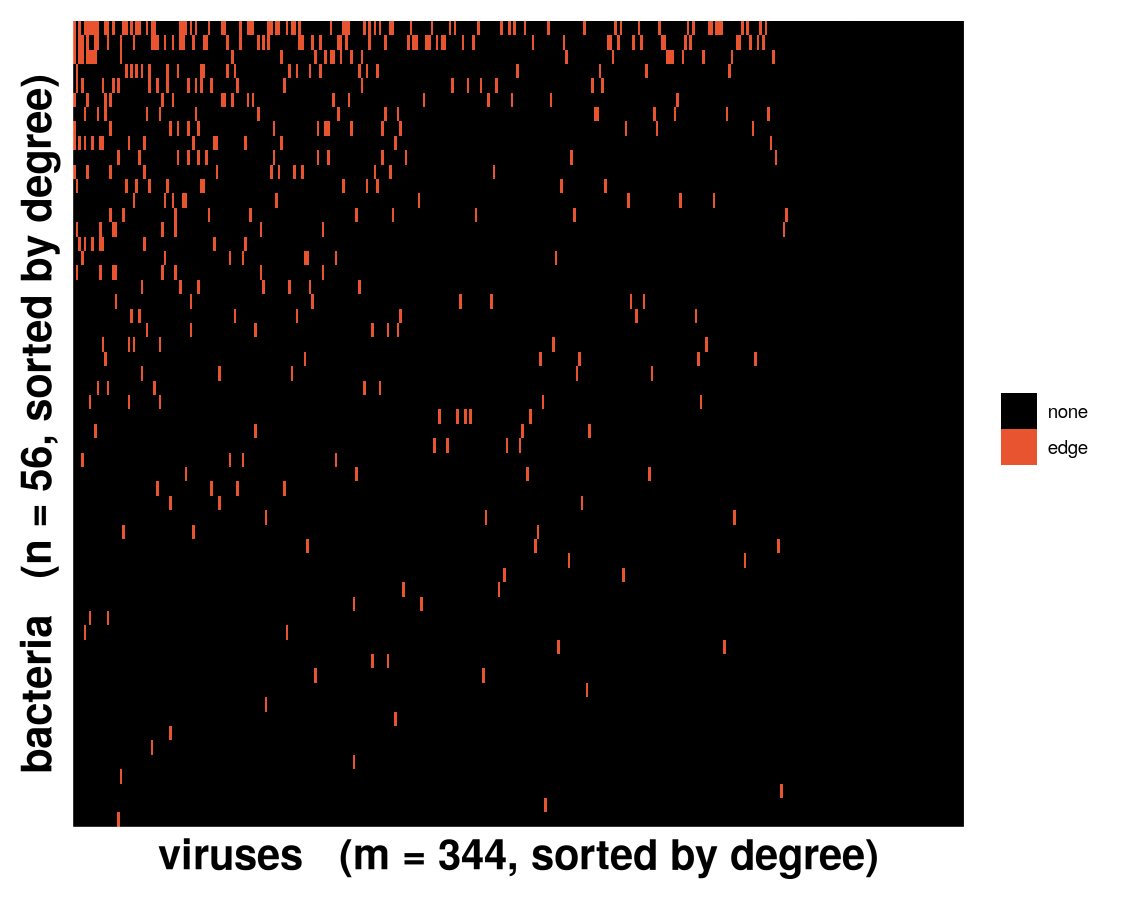
\includegraphics[width=\linewidth]{figures/fig_ap_interaction_Y_matrix_observed_gvhd.png}
    \caption{GvHD}
  \end{subfigure}
  \caption{CRISPR linkage on the observed pairs}
  \label{fig:ap-ymatobs}
\end{figure}

\begin{figure}[H]
  \centering
  \begin{subfigure}[t]{0.32\textwidth}
    \centering
    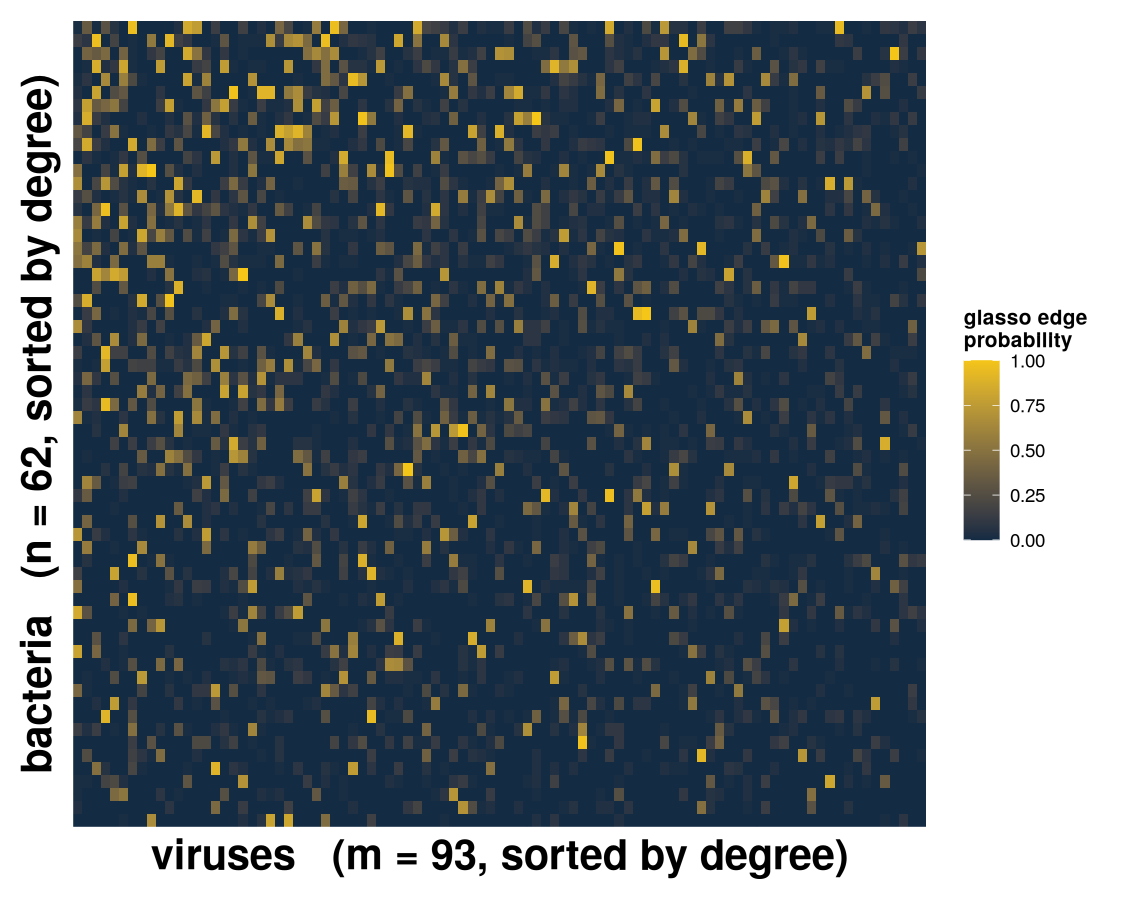
\includegraphics[width=\linewidth]{figures/fig_ap_interaction_W_matrix_observed_crc.png}
    \caption{CRC}
  \end{subfigure}\hfill
  \begin{subfigure}[t]{0.32\textwidth}
    \centering
    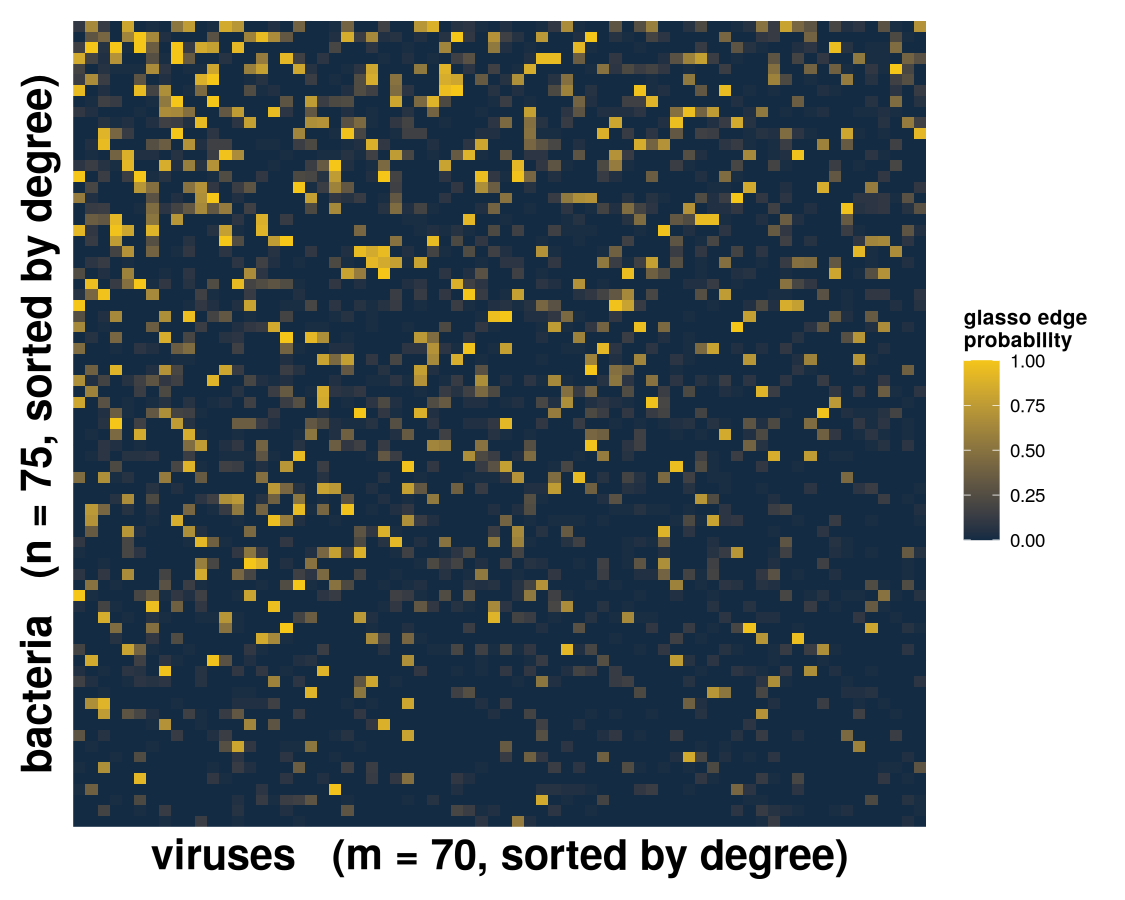
\includegraphics[width=\linewidth]{figures/fig_ap_interaction_W_matrix_observed_ibd.png}
    \caption{IBD}
  \end{subfigure}\hfill
  \begin{subfigure}[t]{0.32\textwidth}
    \centering
    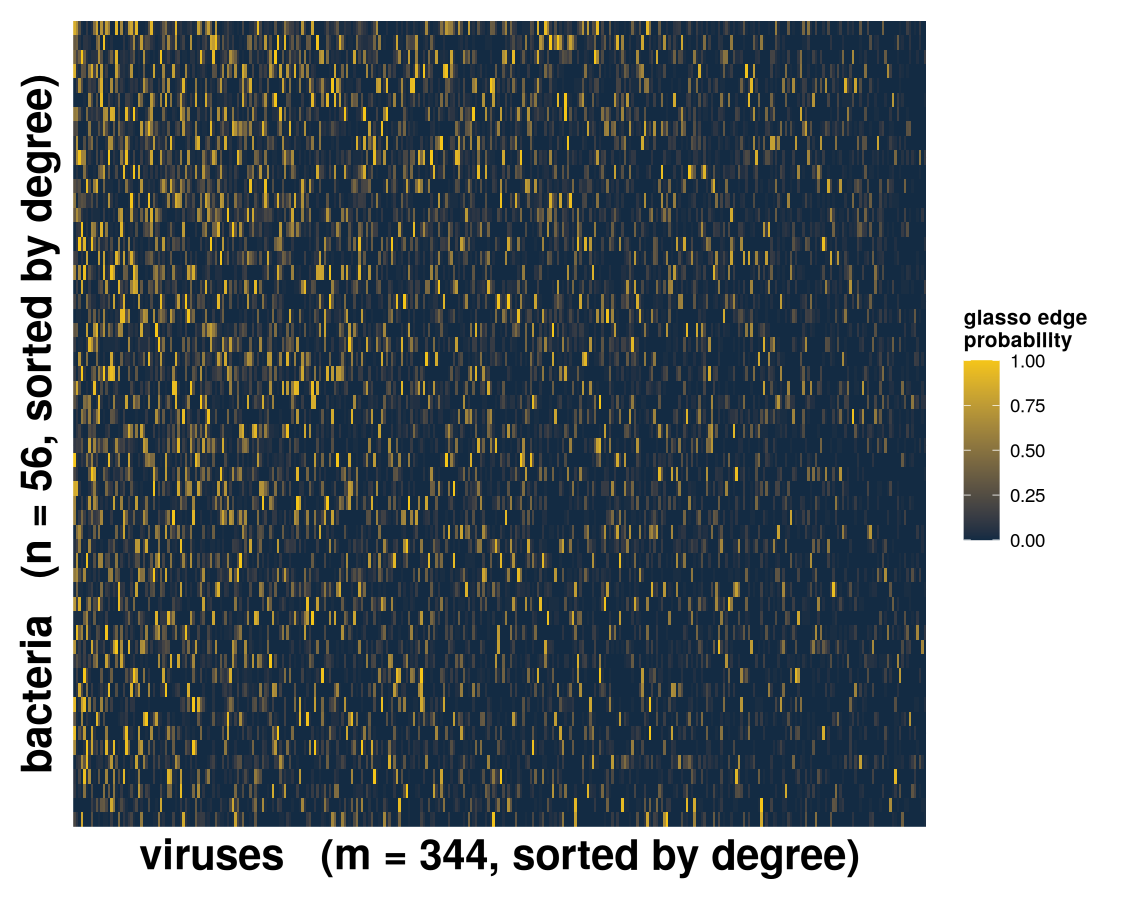
\includegraphics[width=\linewidth]{figures/fig_ap_interaction_W_matrix_observed_gvhd.png}
    \caption{GvHD}
  \end{subfigure}
  \caption{Edge selection probability on the observed pairs}
  \label{fig:ap-wmatobs}
\end{figure}

\begin{figure}[H]
  \centering
  \begin{subfigure}[t]{0.32\textwidth}
    \centering
    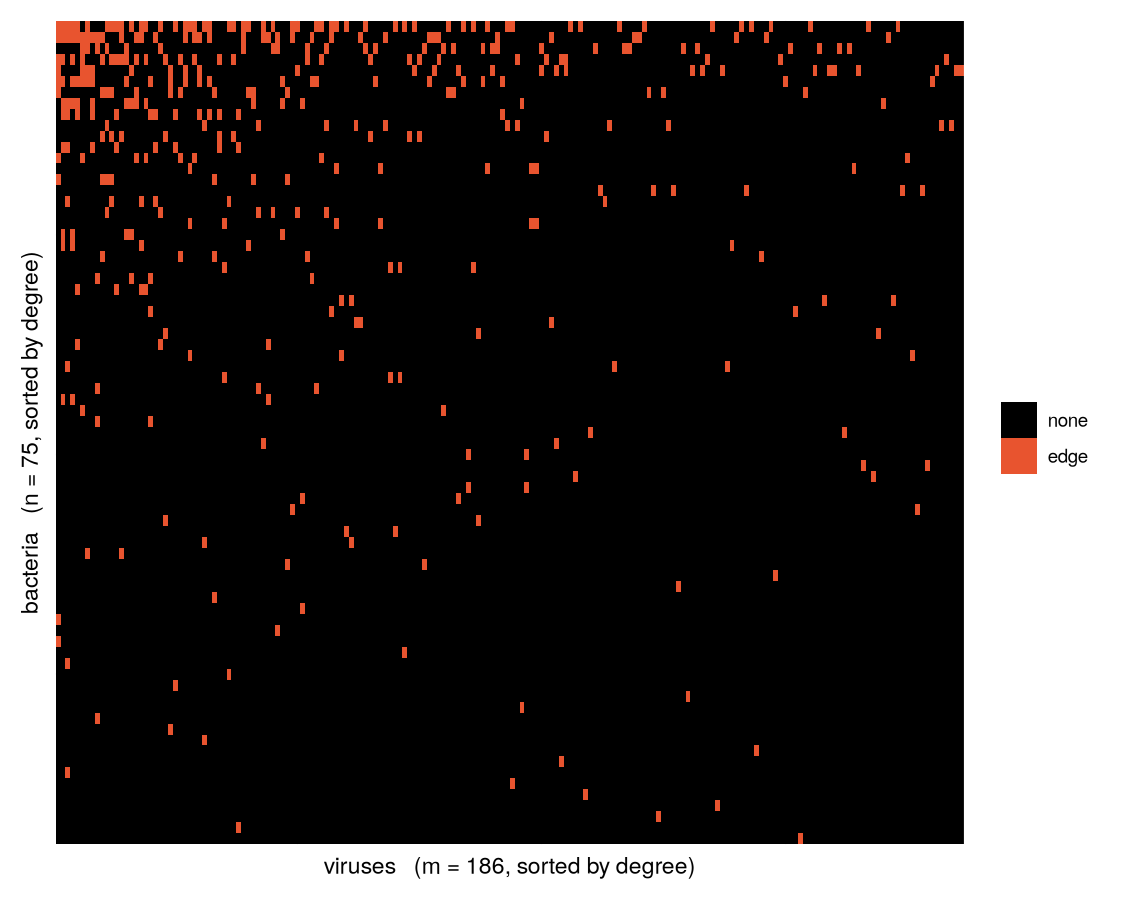
\includegraphics[width=\linewidth]{figures/fig_ap_nestedness_Y_crc.png}
    \caption{CRC}
  \end{subfigure}\hfill
  \begin{subfigure}[t]{0.32\textwidth}
    \centering
    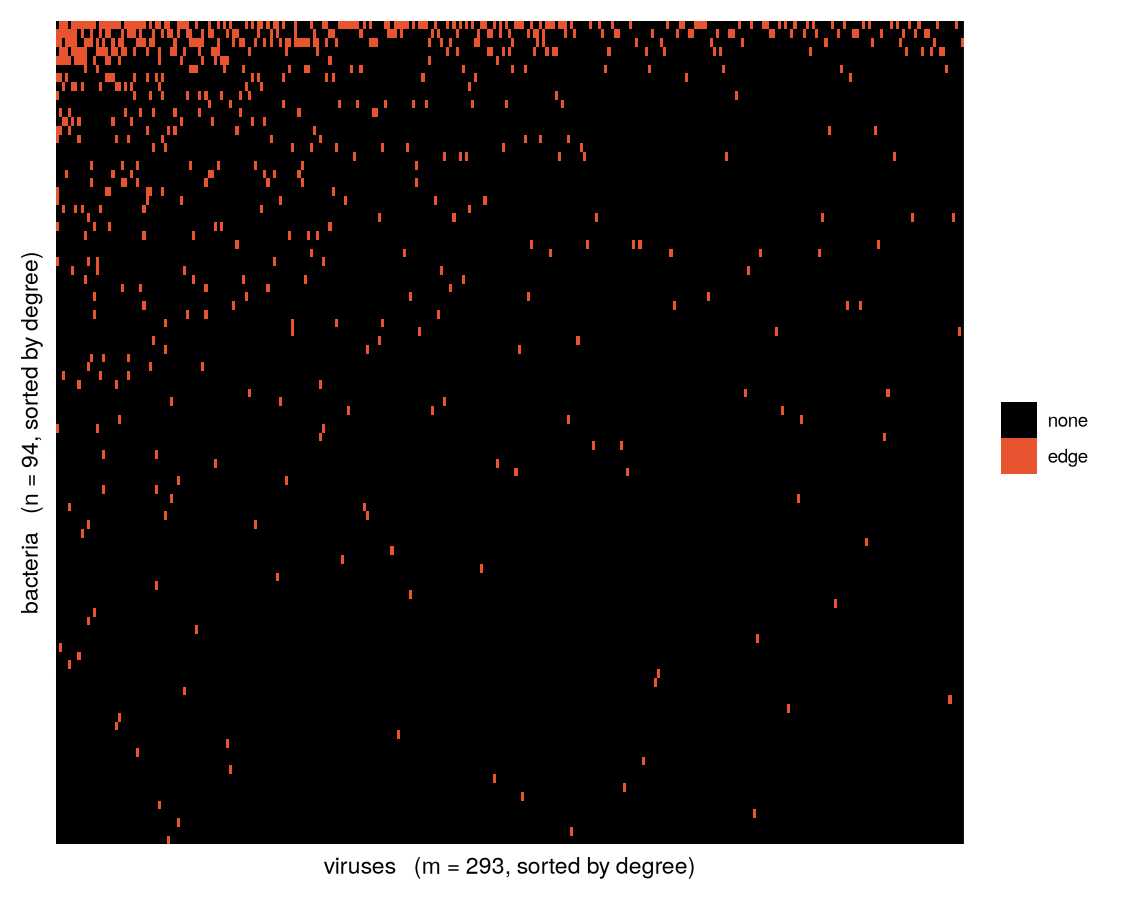
\includegraphics[width=\linewidth]{figures/fig_ap_nestedness_Y_ibd.png}
    \caption{IBD}
  \end{subfigure}\hfill
  \begin{subfigure}[t]{0.32\textwidth}
    \centering
    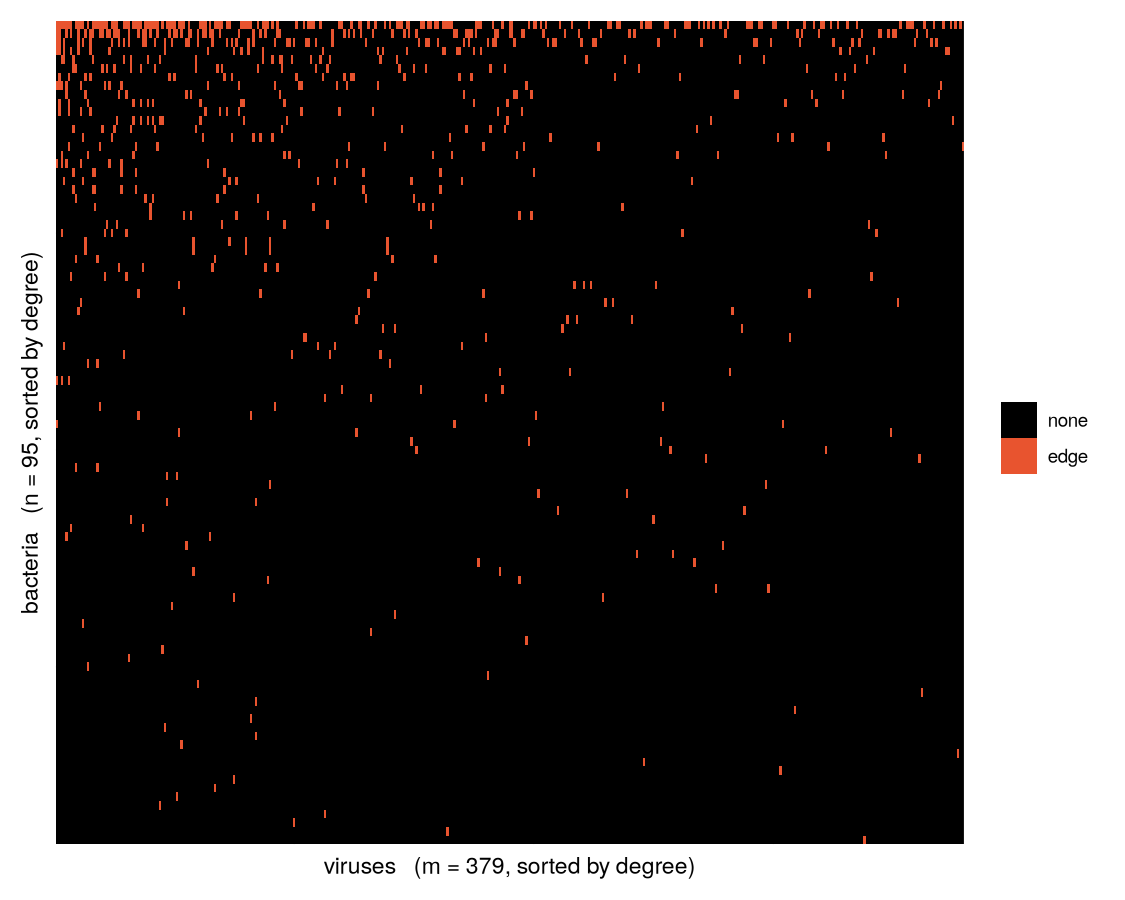
\includegraphics[width=\linewidth]{figures/fig_ap_nestedness_Y_gvhd.png}
    \caption{GvHD}
  \end{subfigure}
  \caption{Nestedness of the CRISPR linkage}
  \label{fig:ap-nesty}
\end{figure}

\begin{figure}[H]
  \centering
  \begin{subfigure}[t]{0.32\textwidth}
    \centering
    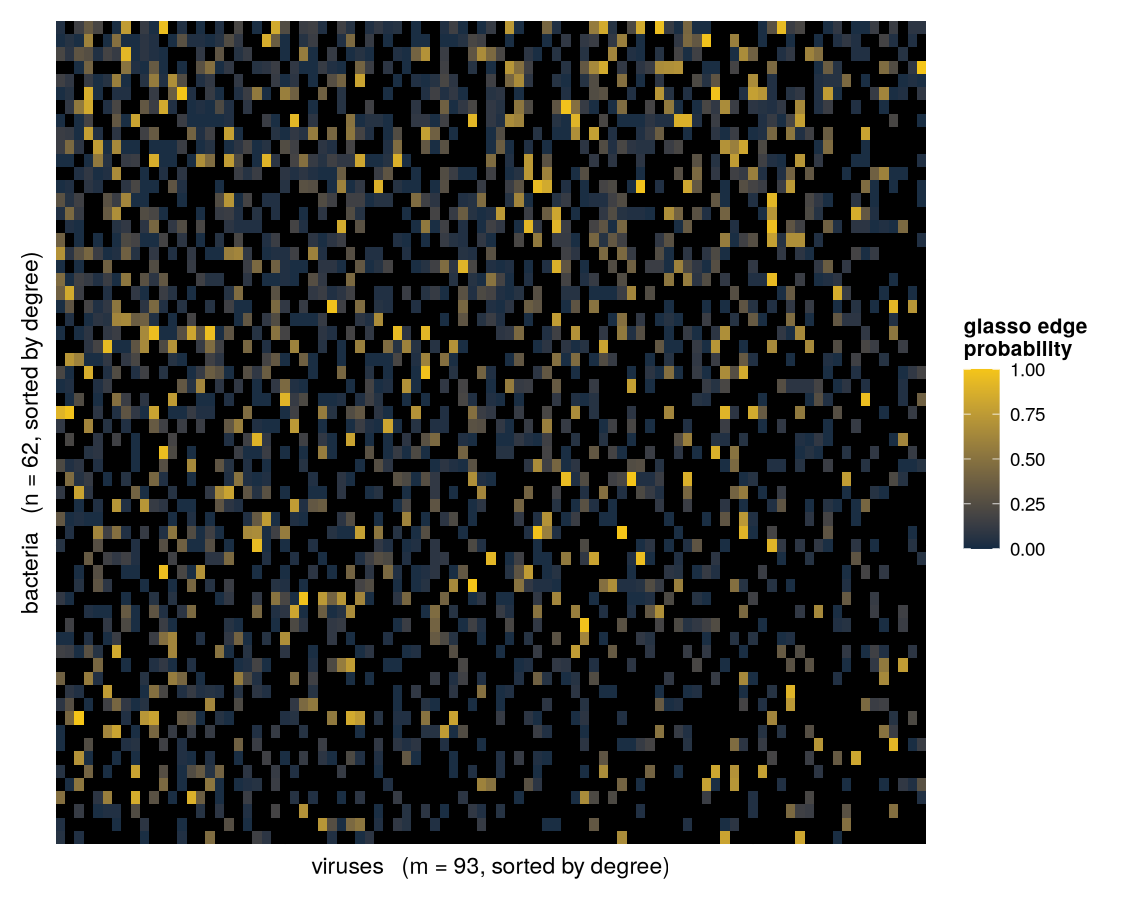
\includegraphics[width=\linewidth]{figures/fig_ap_nestedness_W_crc.png}
    \caption{CRC}
  \end{subfigure}\hfill
  \begin{subfigure}[t]{0.32\textwidth}
    \centering
    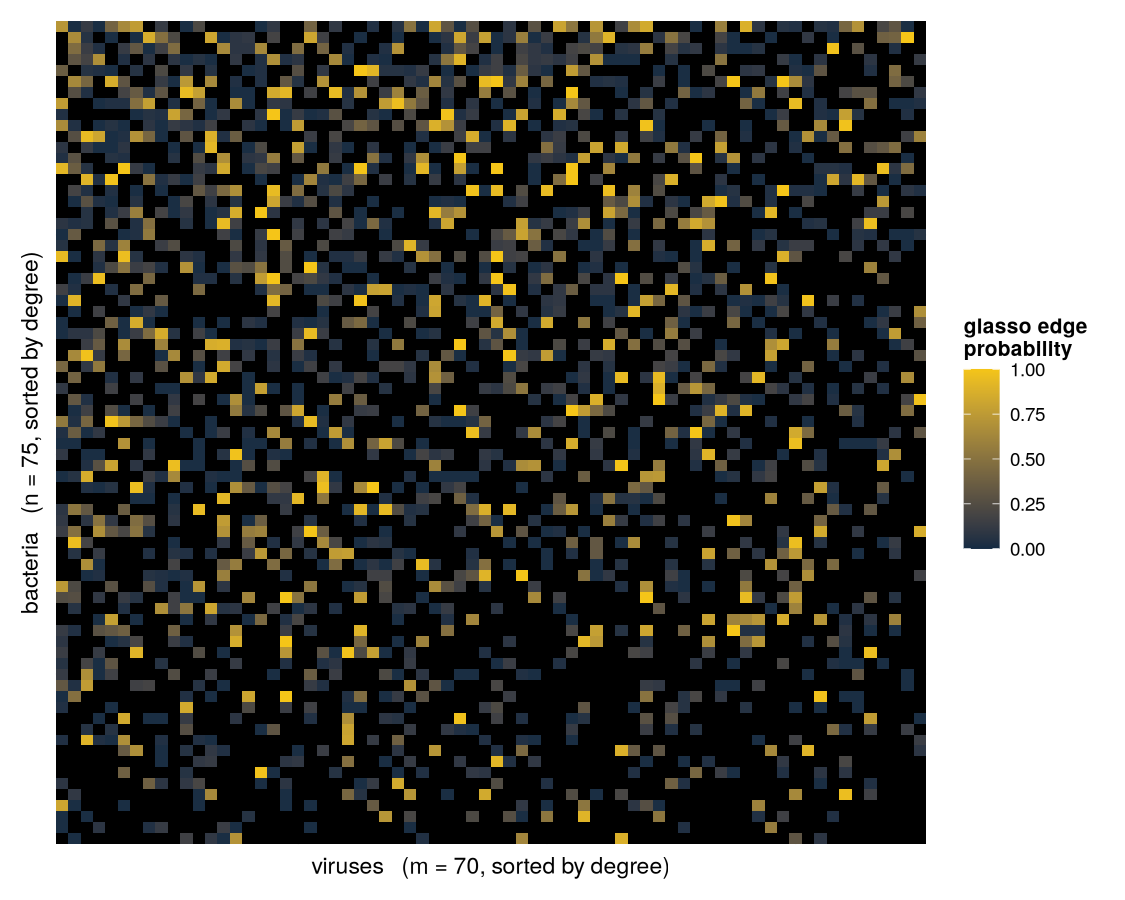
\includegraphics[width=\linewidth]{figures/fig_ap_nestedness_W_ibd.png}
    \caption{IBD}
  \end{subfigure}\hfill
  \begin{subfigure}[t]{0.32\textwidth}
    \centering
    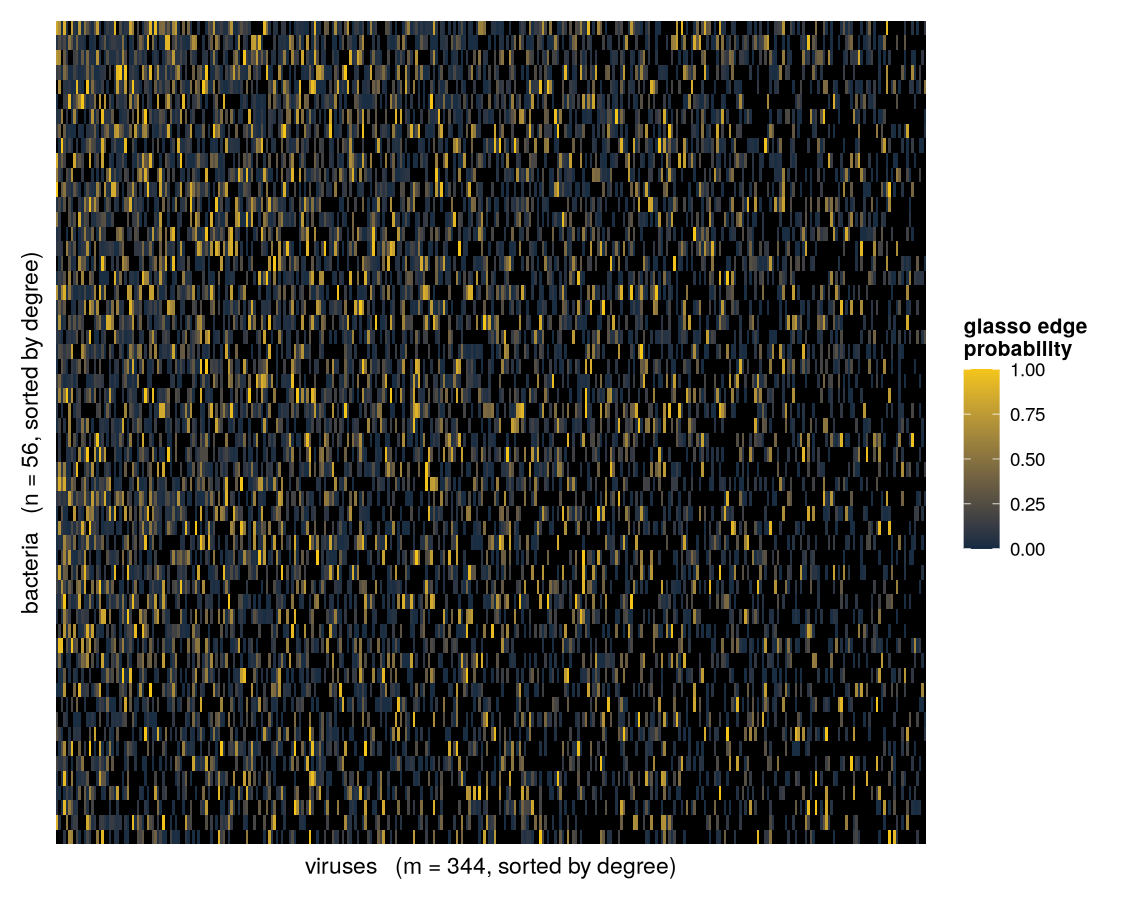
\includegraphics[width=\linewidth]{figures/fig_ap_nestedness_W_gvhd.png}
    \caption{GvHD}
  \end{subfigure}
  \caption{Nestedness of the edge selection probability}
  \label{fig:ap-nestw}
\end{figure}

\subsection{Test Scores by Model}

\begin{figure}[H]
  \centering
  \begin{subfigure}[t]{0.32\textwidth}
    \centering
    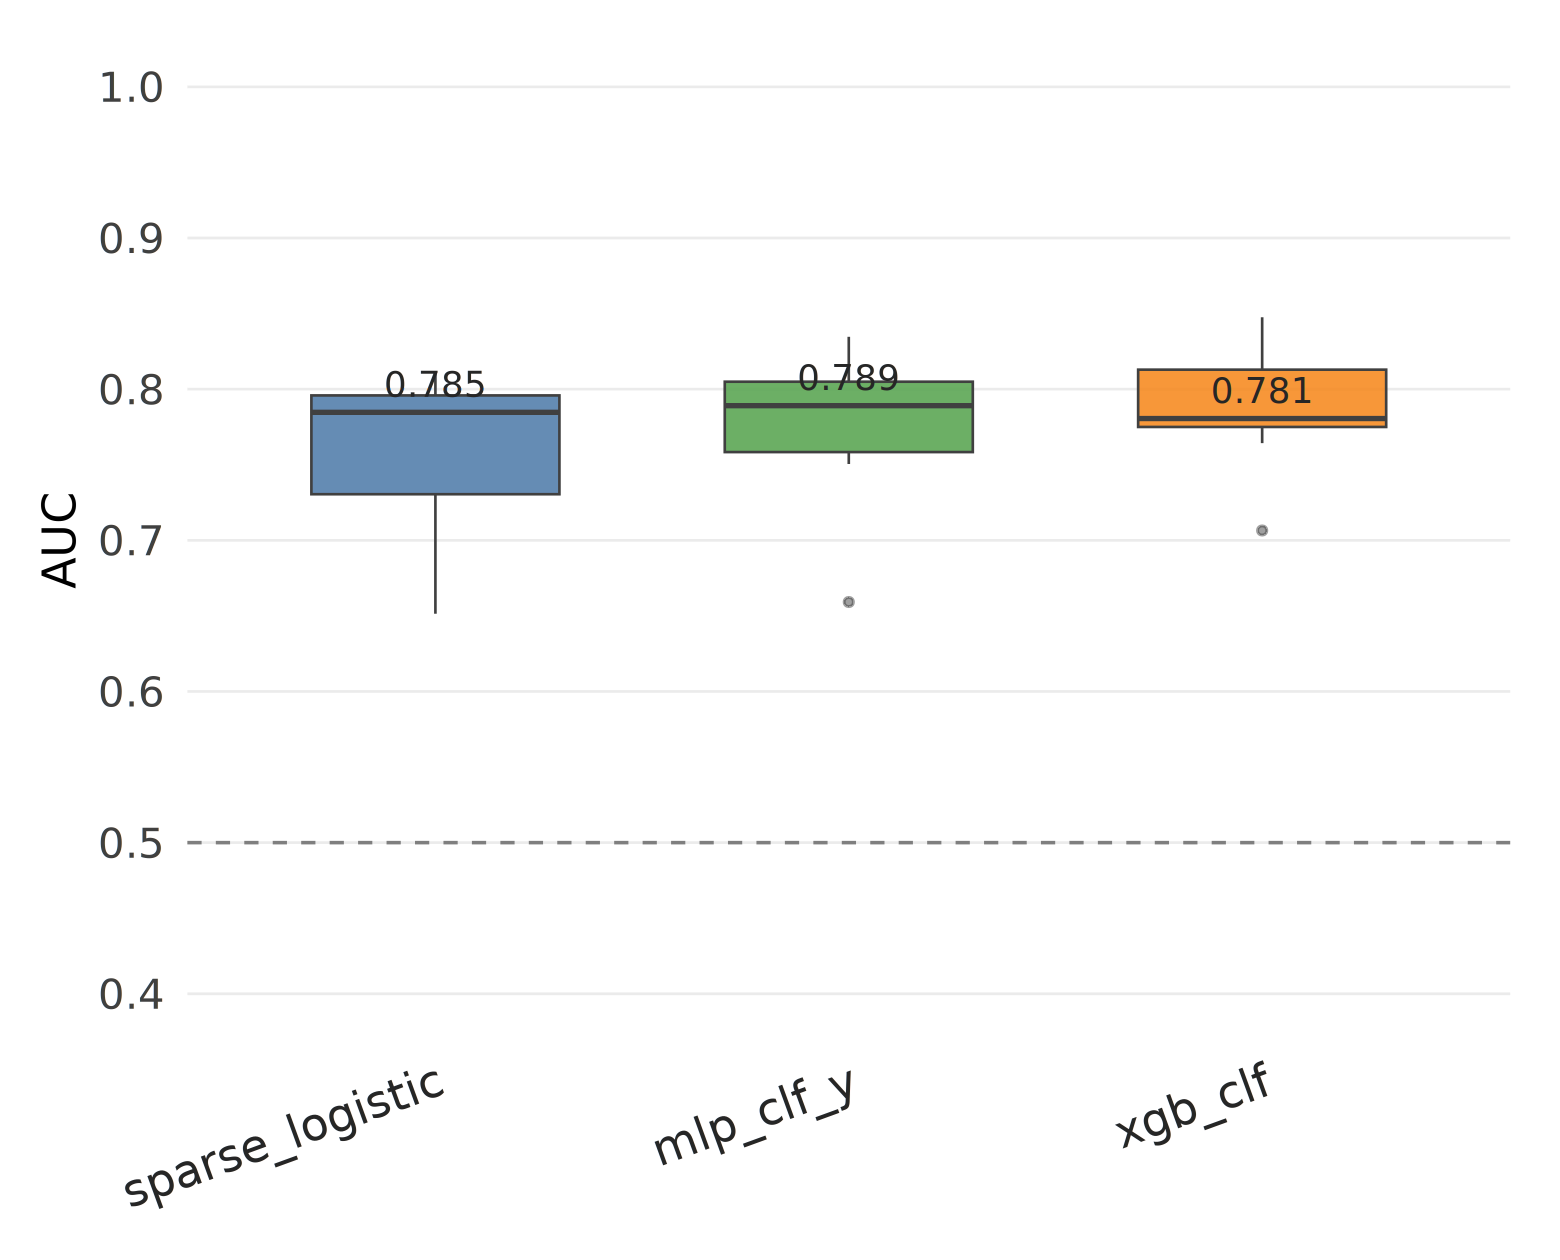
\includegraphics[width=\linewidth]{figures/fig_ap_y_auc_baseline_crc.png}
    \caption{CRC}
  \end{subfigure}\hfill
  \begin{subfigure}[t]{0.32\textwidth}
    \centering
    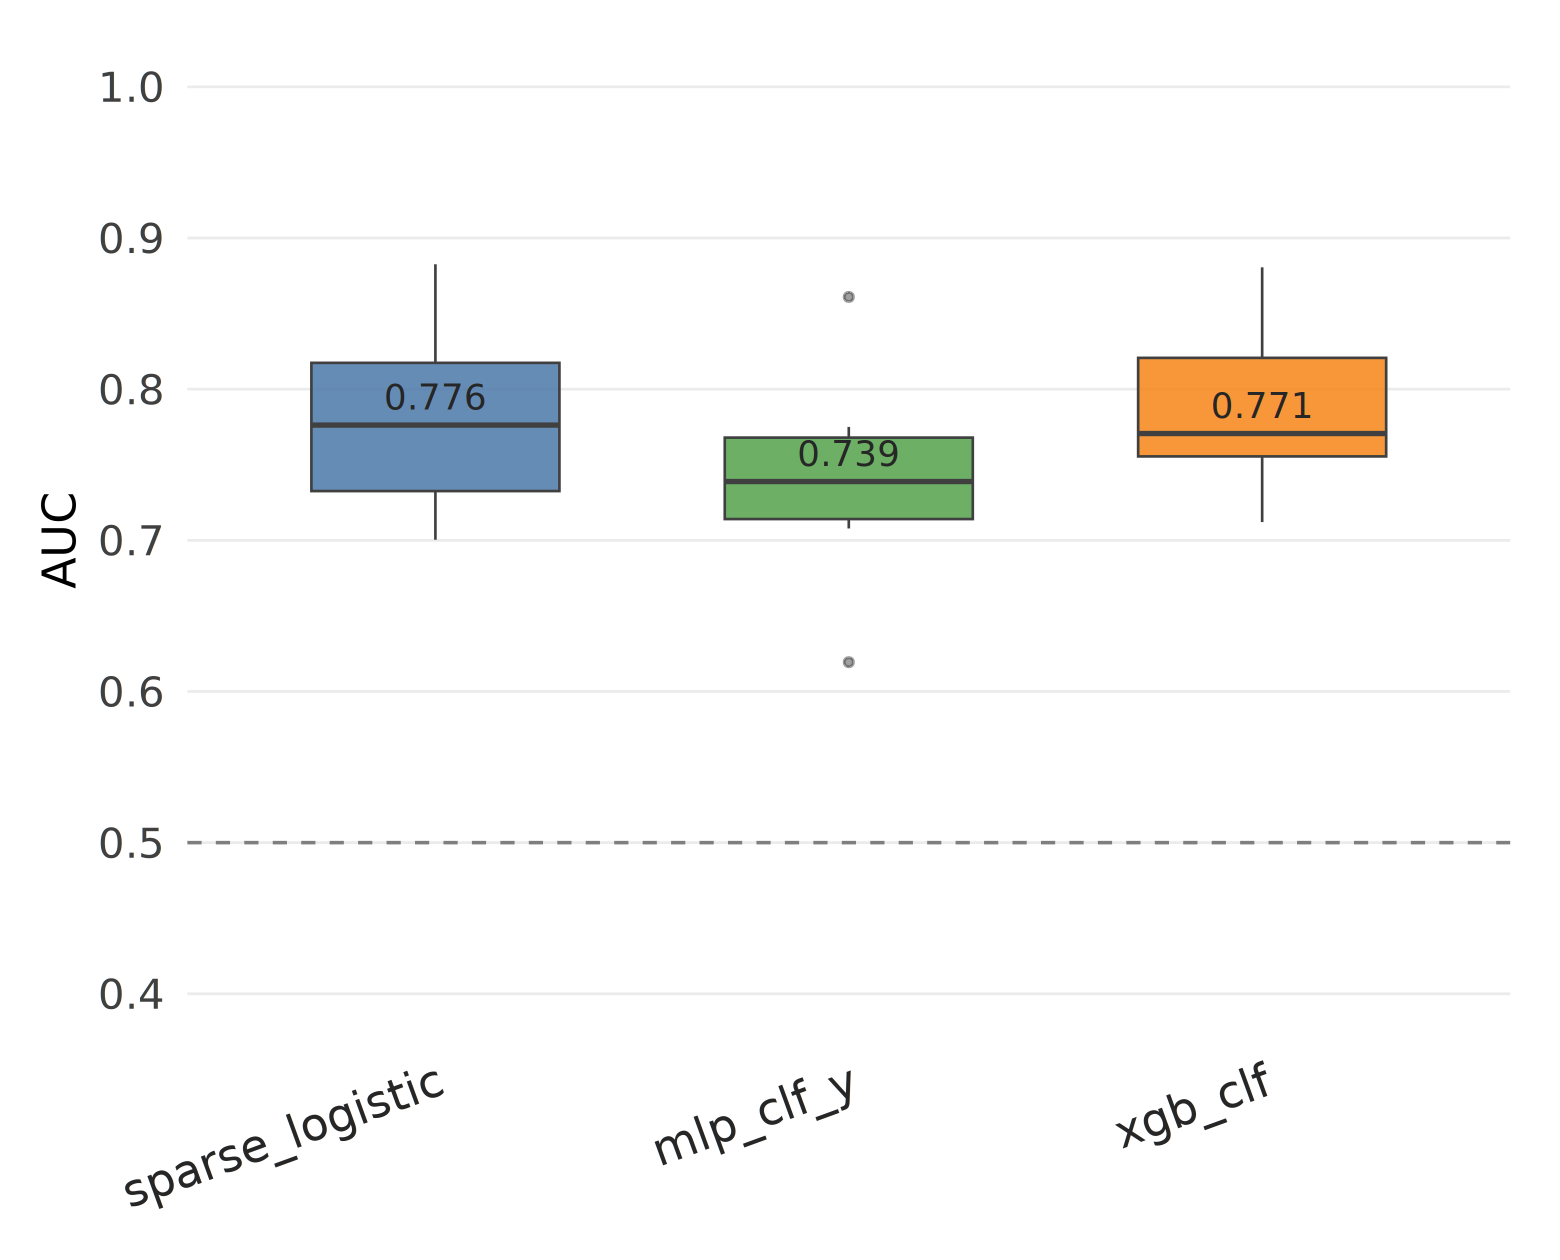
\includegraphics[width=\linewidth]{figures/fig_ap_y_auc_baseline_ibd.png}
    \caption{IBD}
  \end{subfigure}\hfill
  \begin{subfigure}[t]{0.32\textwidth}
    \centering
    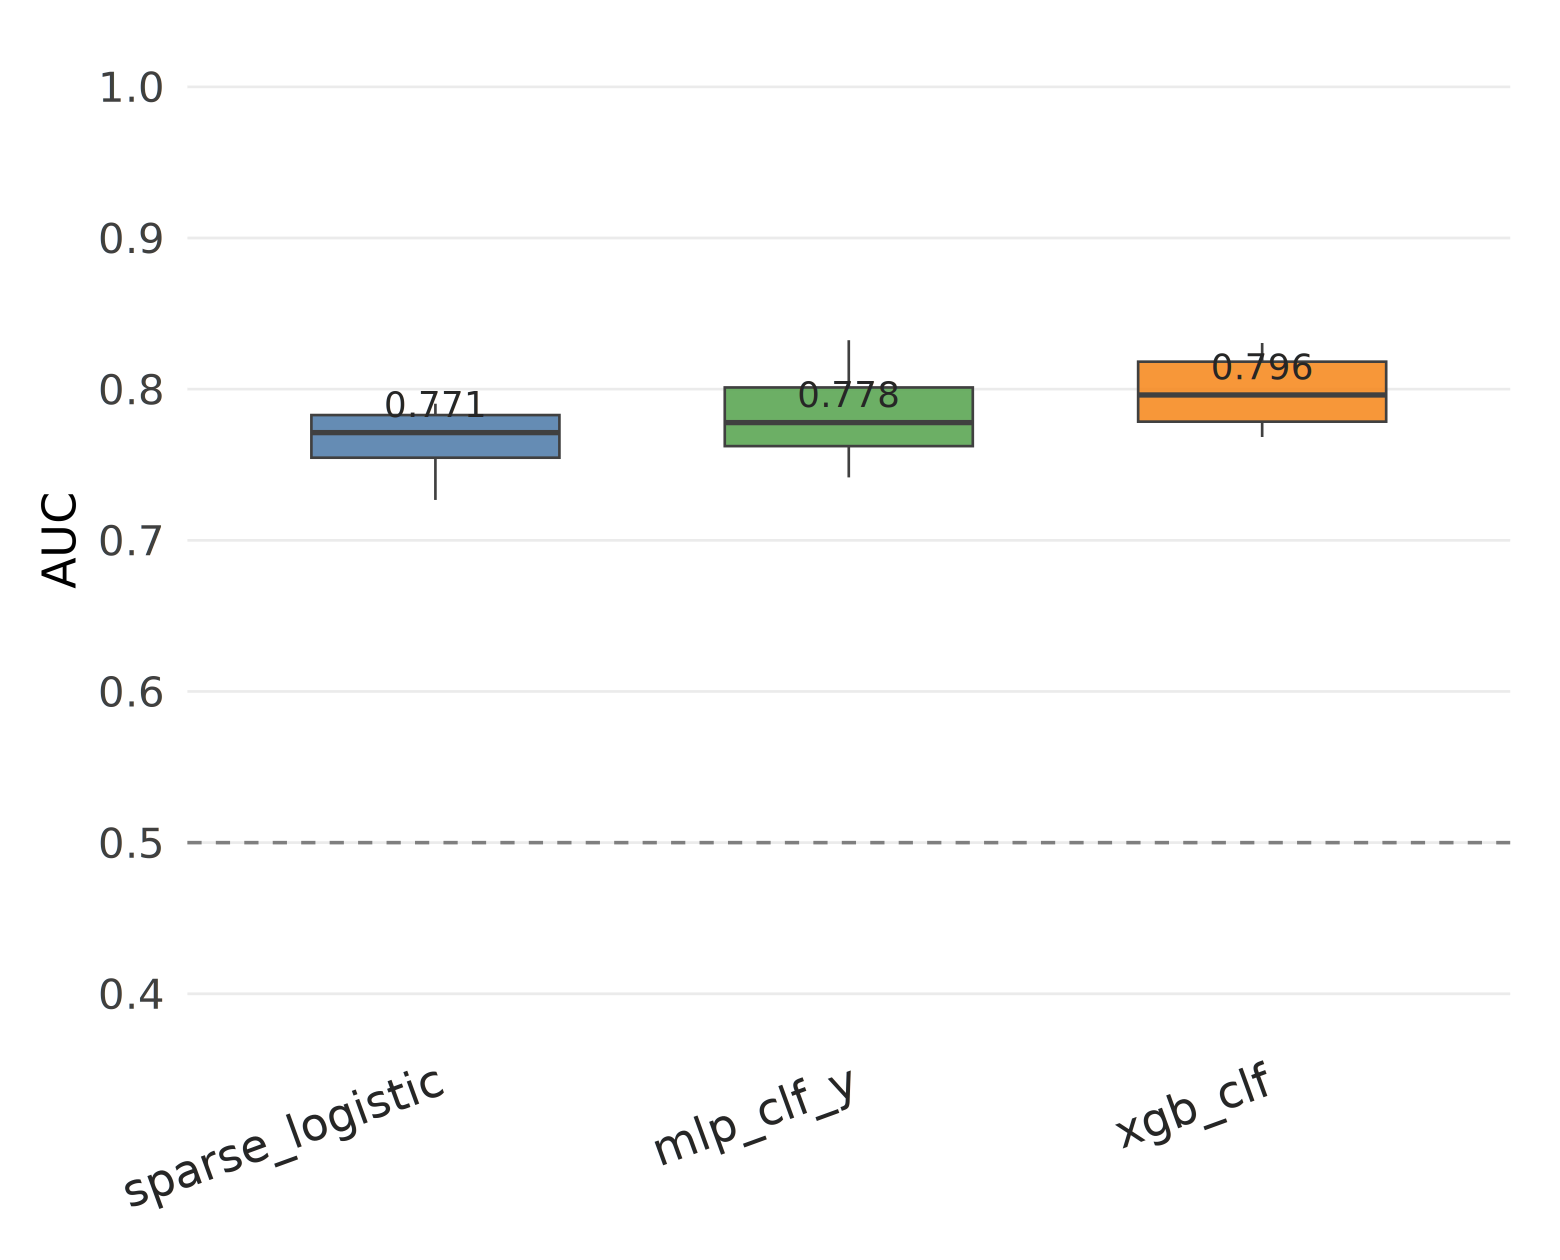
\includegraphics[width=\linewidth]{figures/fig_ap_y_auc_baseline_gvhd.png}
    \caption{GvHD}
  \end{subfigure}
  \caption{Test AUC on CRISPR linkage, baseline models}
  \label{fig:ap-yaucb}
\end{figure}

\begin{figure}[H]
  \centering
  \begin{subfigure}[t]{0.32\textwidth}
    \centering
    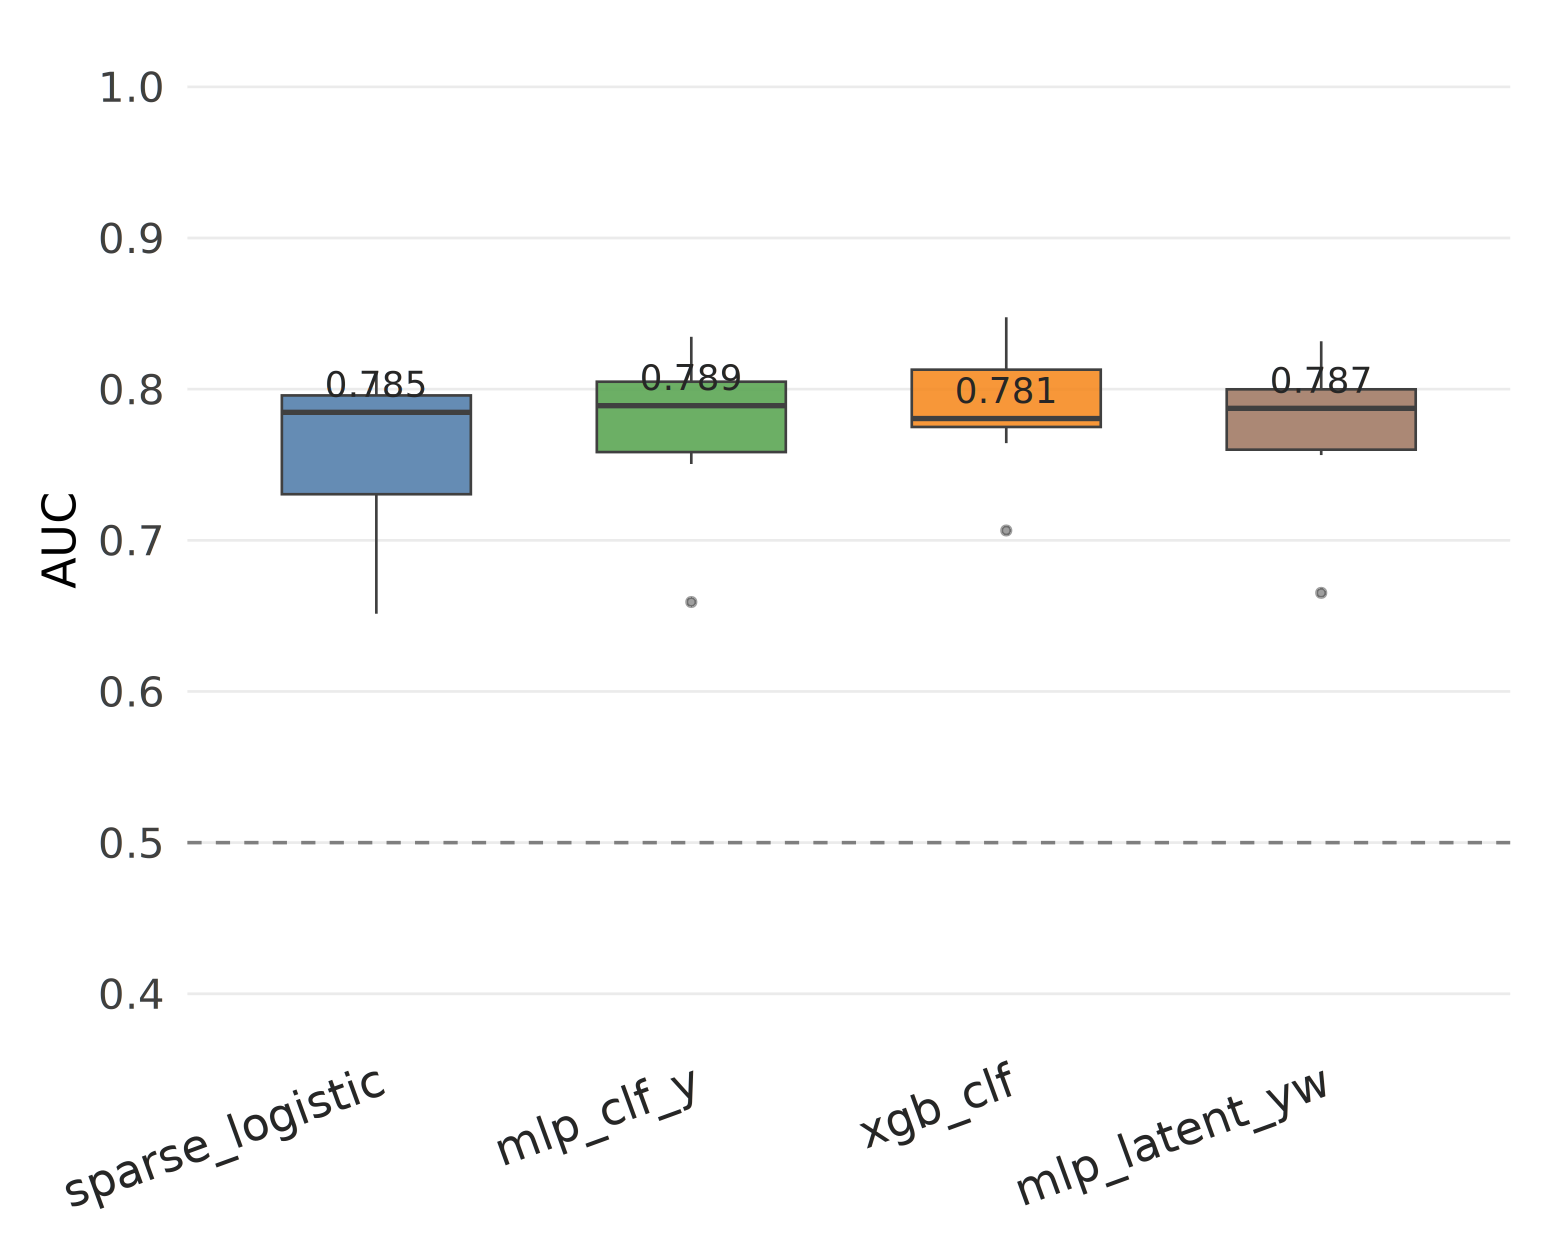
\includegraphics[width=\linewidth]{figures/fig_ap_y_auc_all_crc.png}
    \caption{CRC}
  \end{subfigure}\hfill
  \begin{subfigure}[t]{0.32\textwidth}
    \centering
    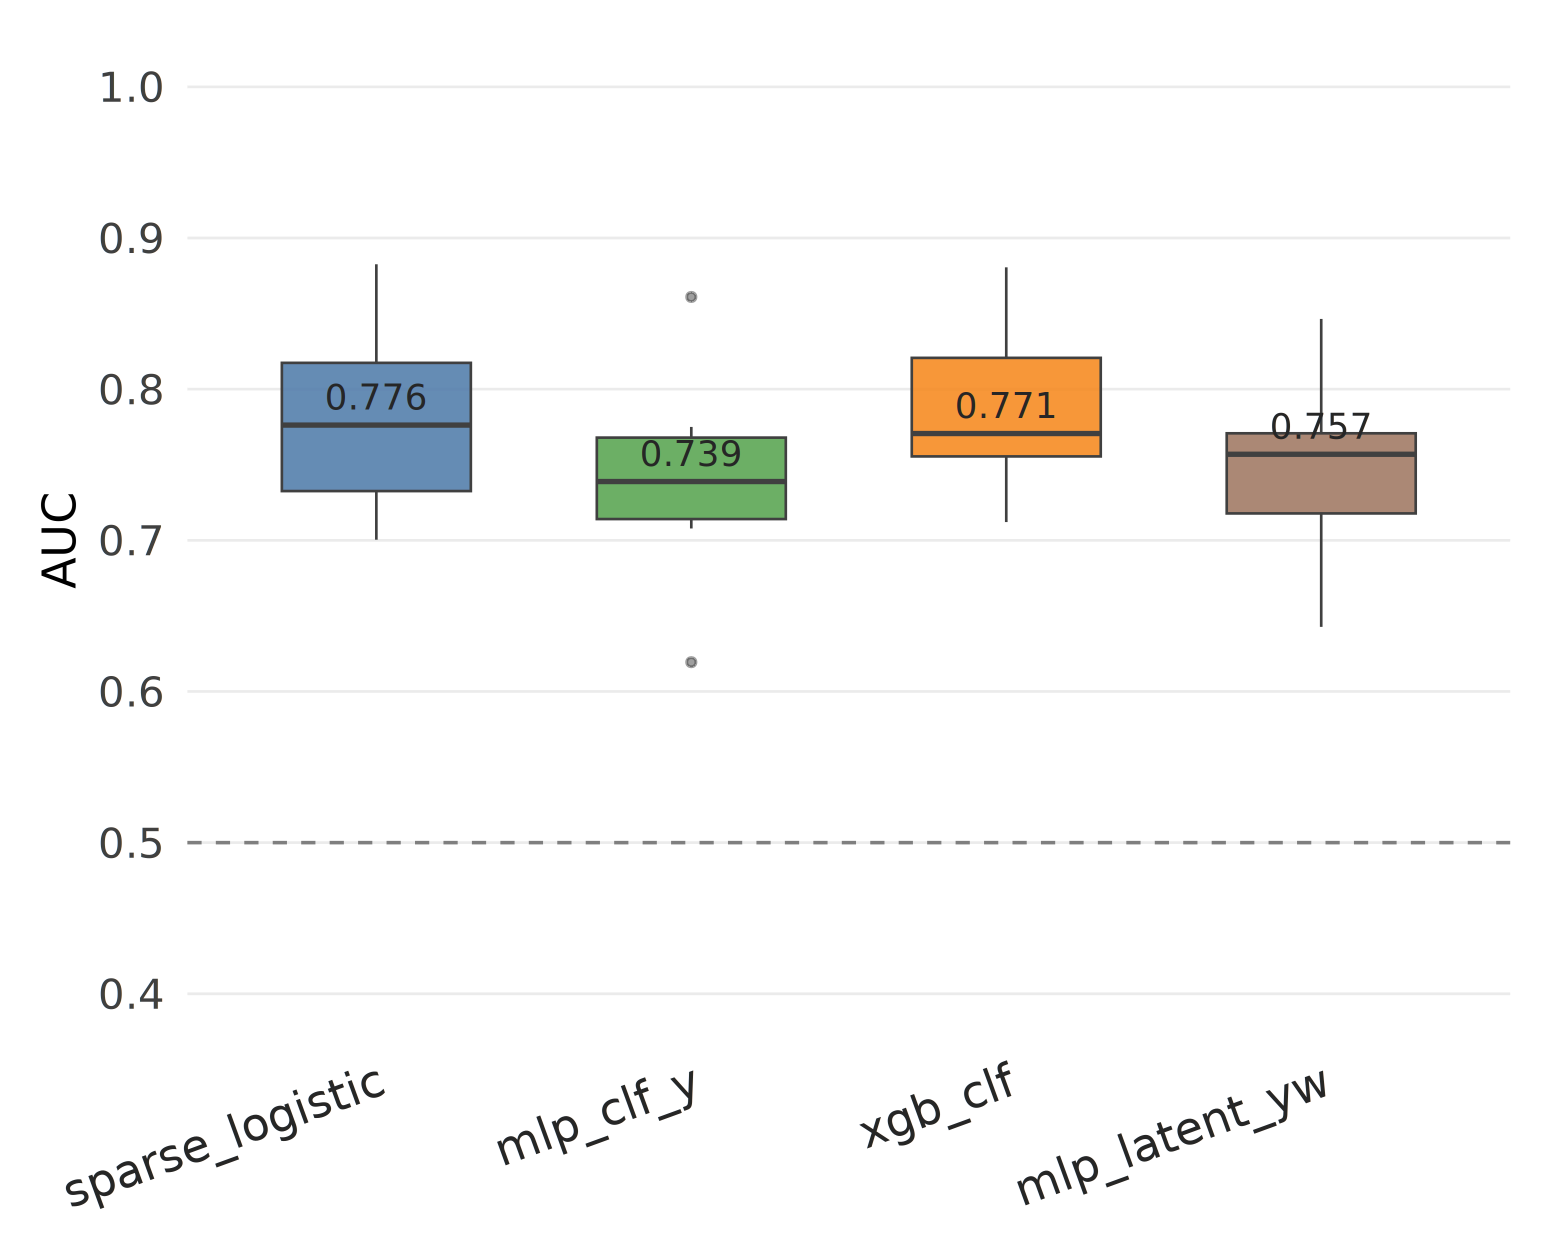
\includegraphics[width=\linewidth]{figures/fig_ap_y_auc_all_ibd.png}
    \caption{IBD}
  \end{subfigure}\hfill
  \begin{subfigure}[t]{0.32\textwidth}
    \centering
    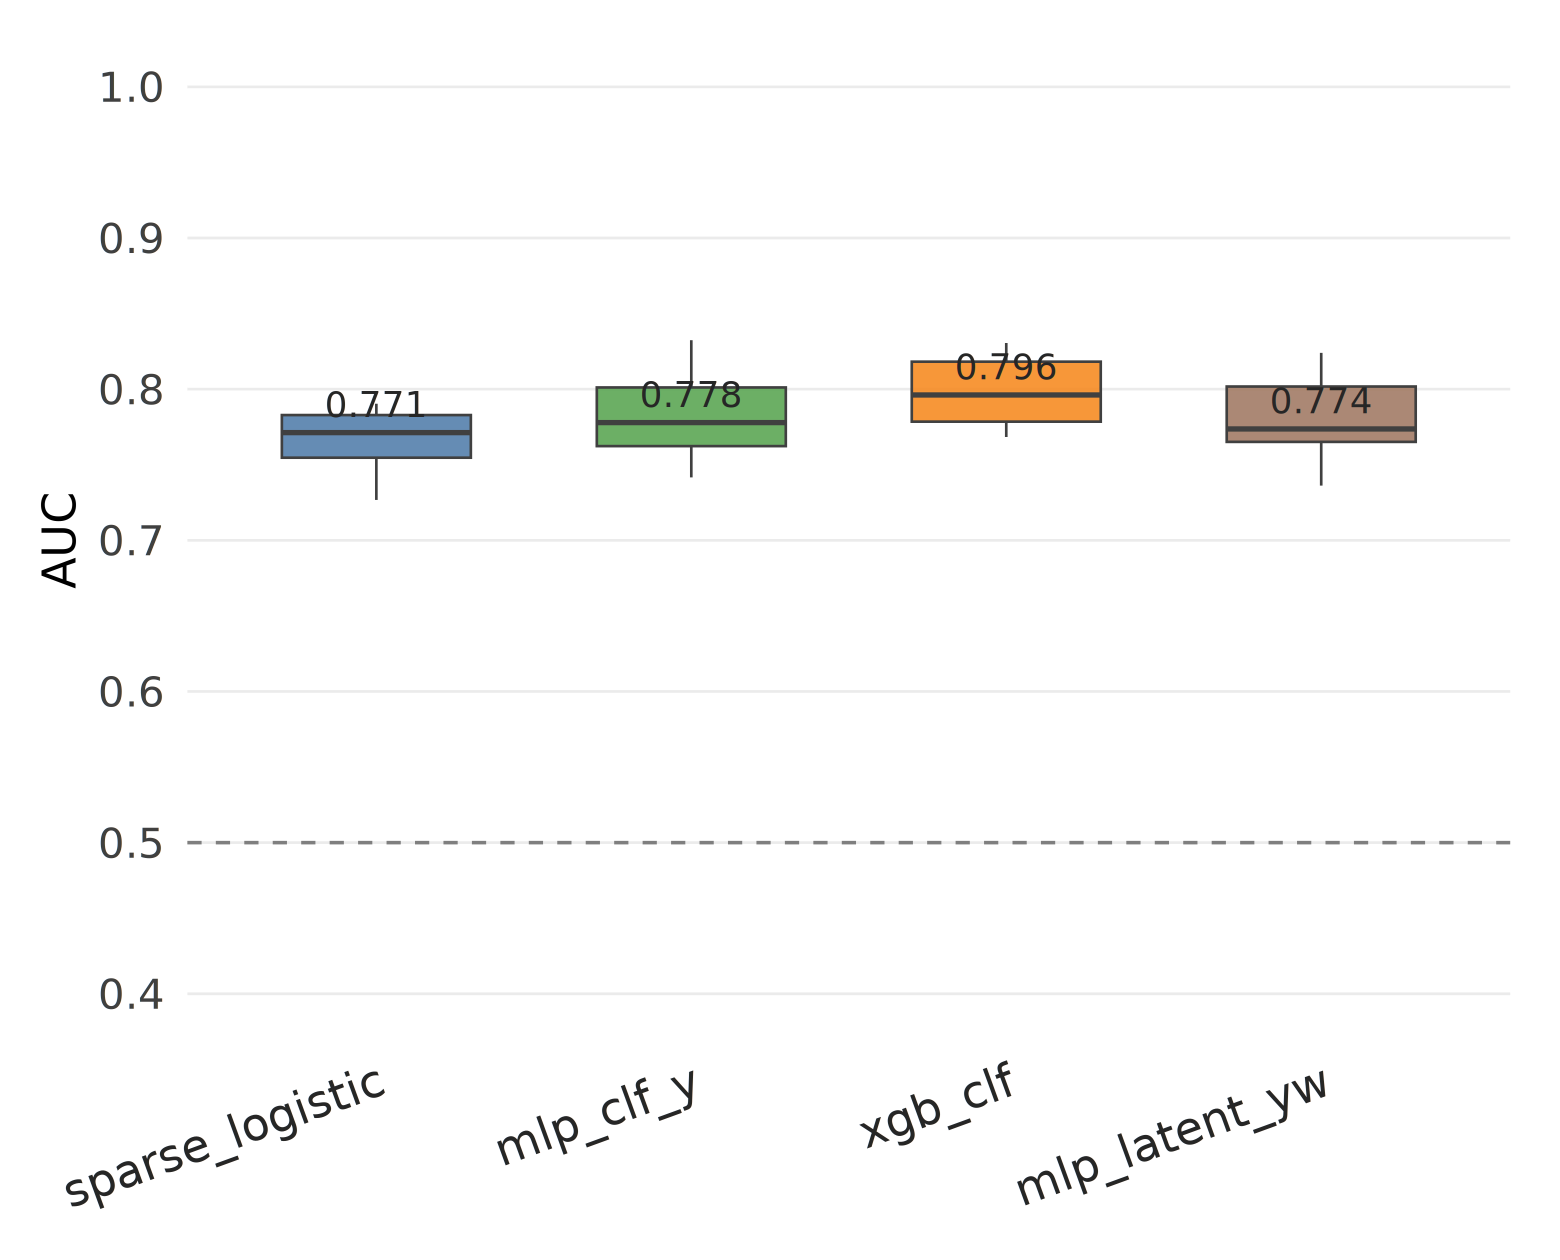
\includegraphics[width=\linewidth]{figures/fig_ap_y_auc_all_gvhd.png}
    \caption{GvHD}
  \end{subfigure}
  \caption{Test AUC on CRISPR linkage, all models}
  \label{fig:ap-yauca}
\end{figure}

\begin{figure}[H]
  \centering
  \begin{subfigure}[t]{0.32\textwidth}
    \centering
    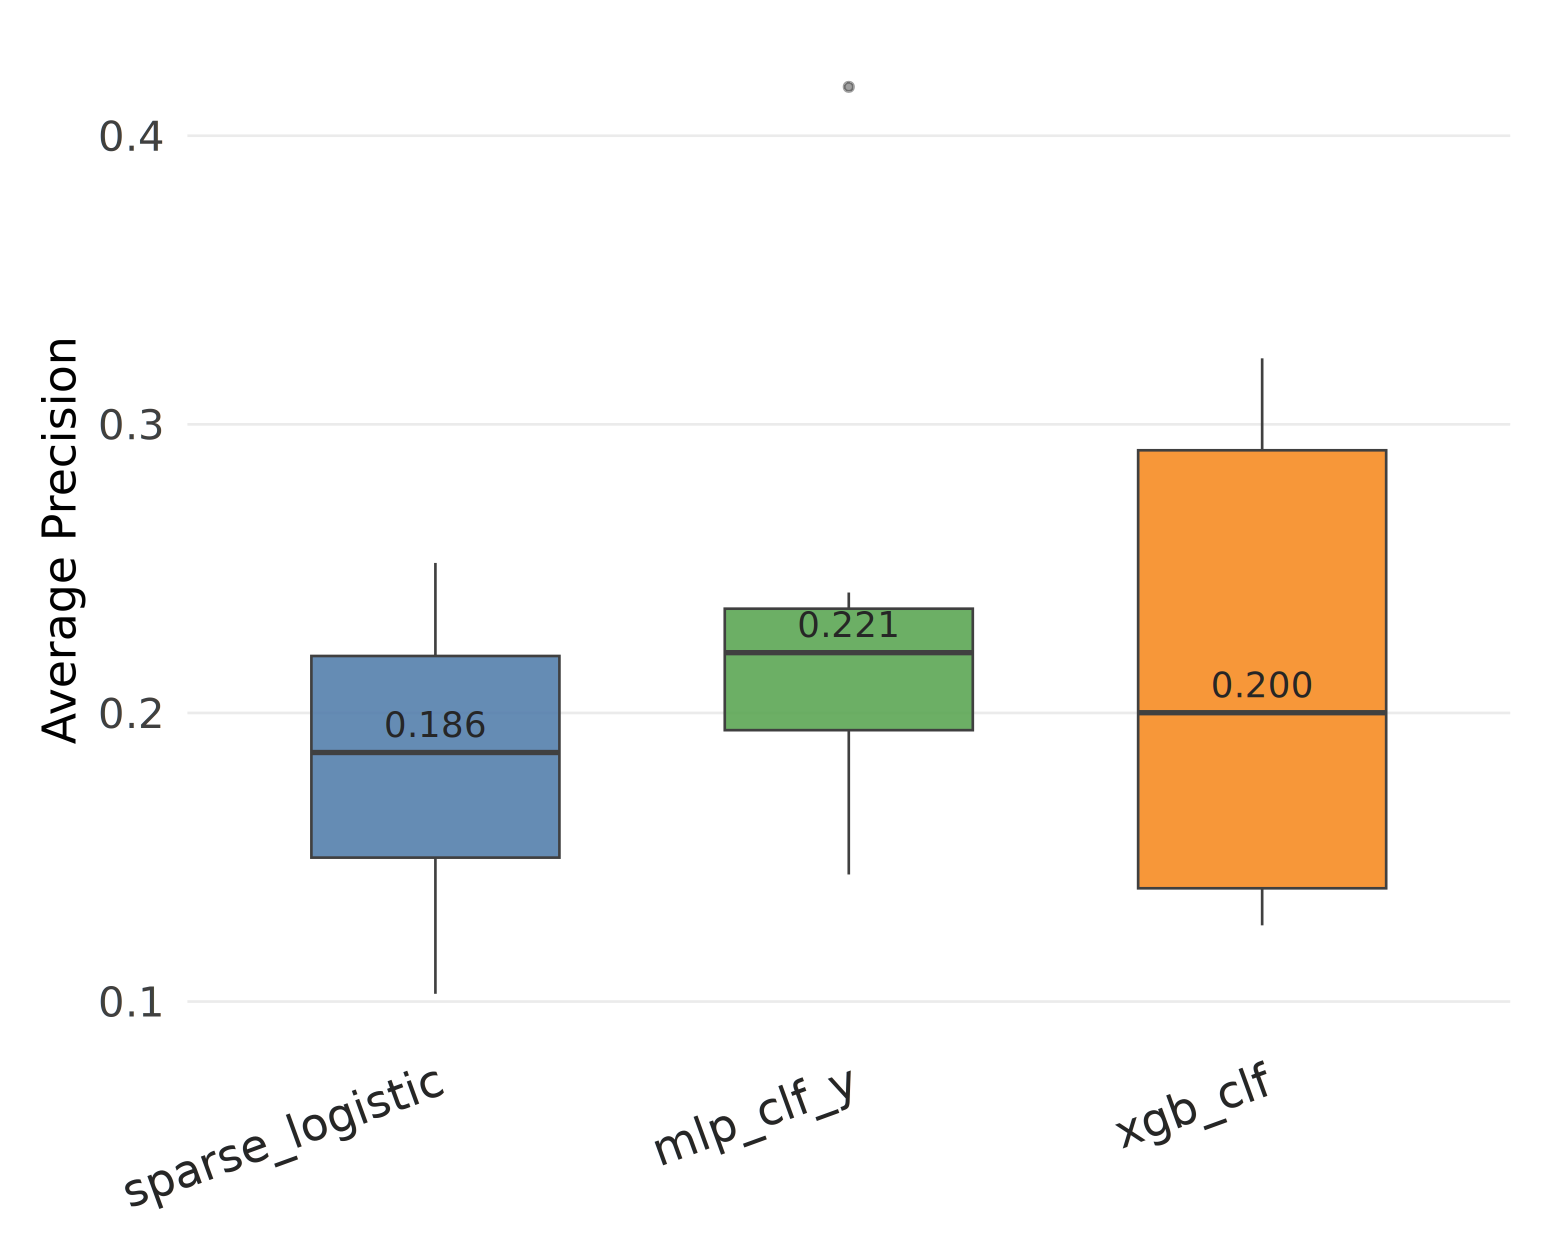
\includegraphics[width=\linewidth]{figures/fig_ap_y_ap_baseline_crc.png}
    \caption{CRC}
  \end{subfigure}\hfill
  \begin{subfigure}[t]{0.32\textwidth}
    \centering
    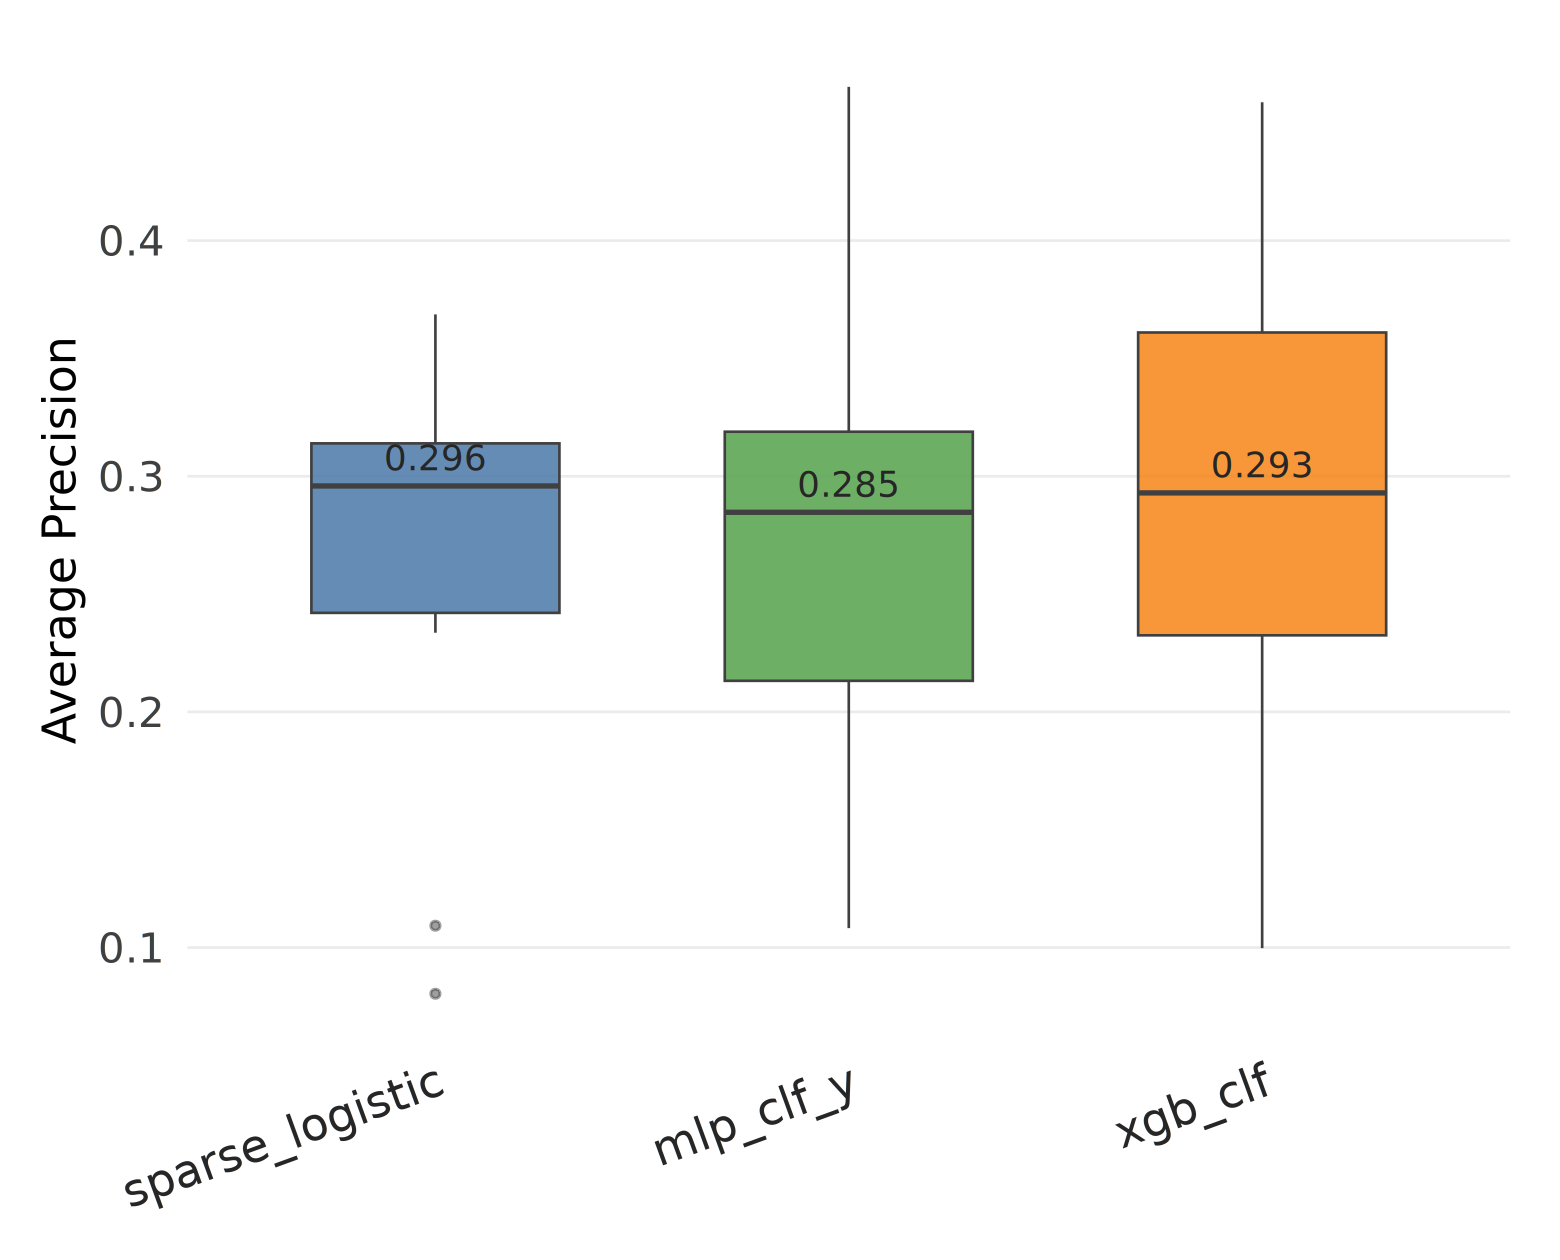
\includegraphics[width=\linewidth]{figures/fig_ap_y_ap_baseline_ibd.png}
    \caption{IBD}
  \end{subfigure}\hfill
  \begin{subfigure}[t]{0.32\textwidth}
    \centering
    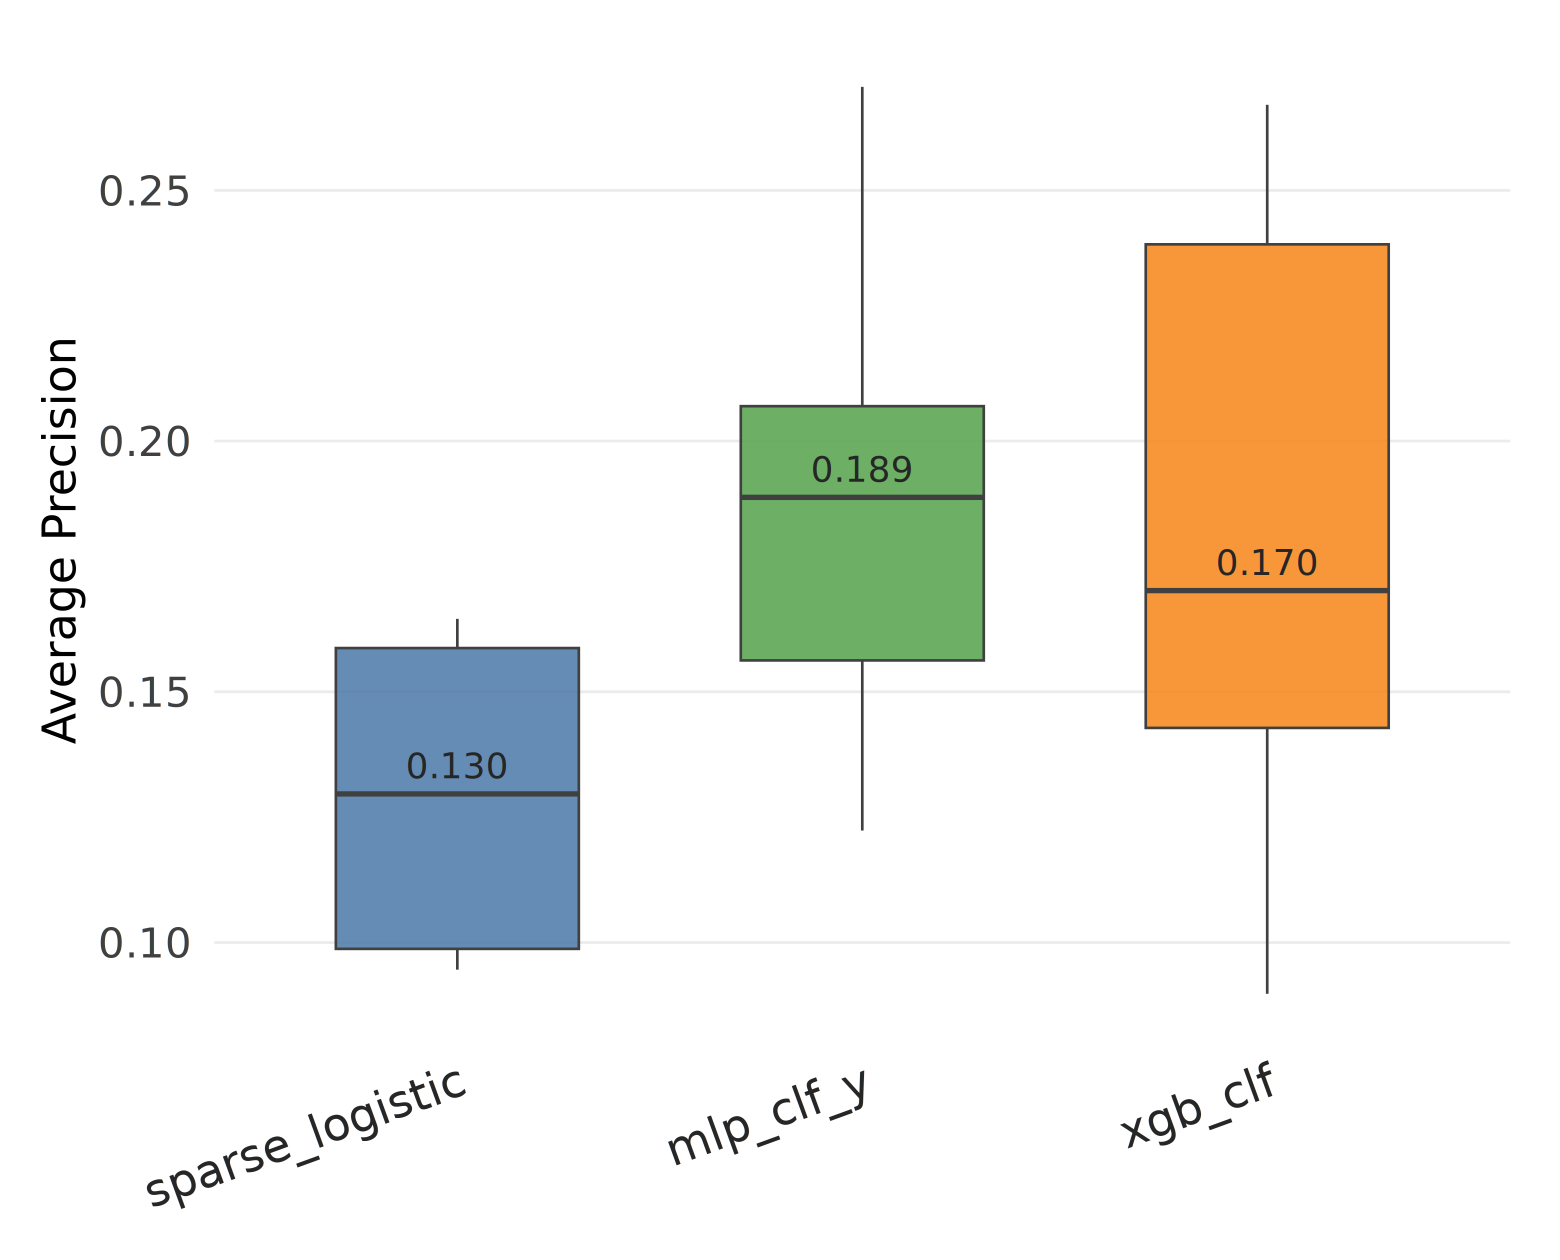
\includegraphics[width=\linewidth]{figures/fig_ap_y_ap_baseline_gvhd.png}
    \caption{GvHD}
  \end{subfigure}
  \caption{Test AP on CRISPR linkage, baseline models}
  \label{fig:ap-yapb}
\end{figure}

\begin{figure}[H]
  \centering
  \begin{subfigure}[t]{0.32\textwidth}
    \centering
    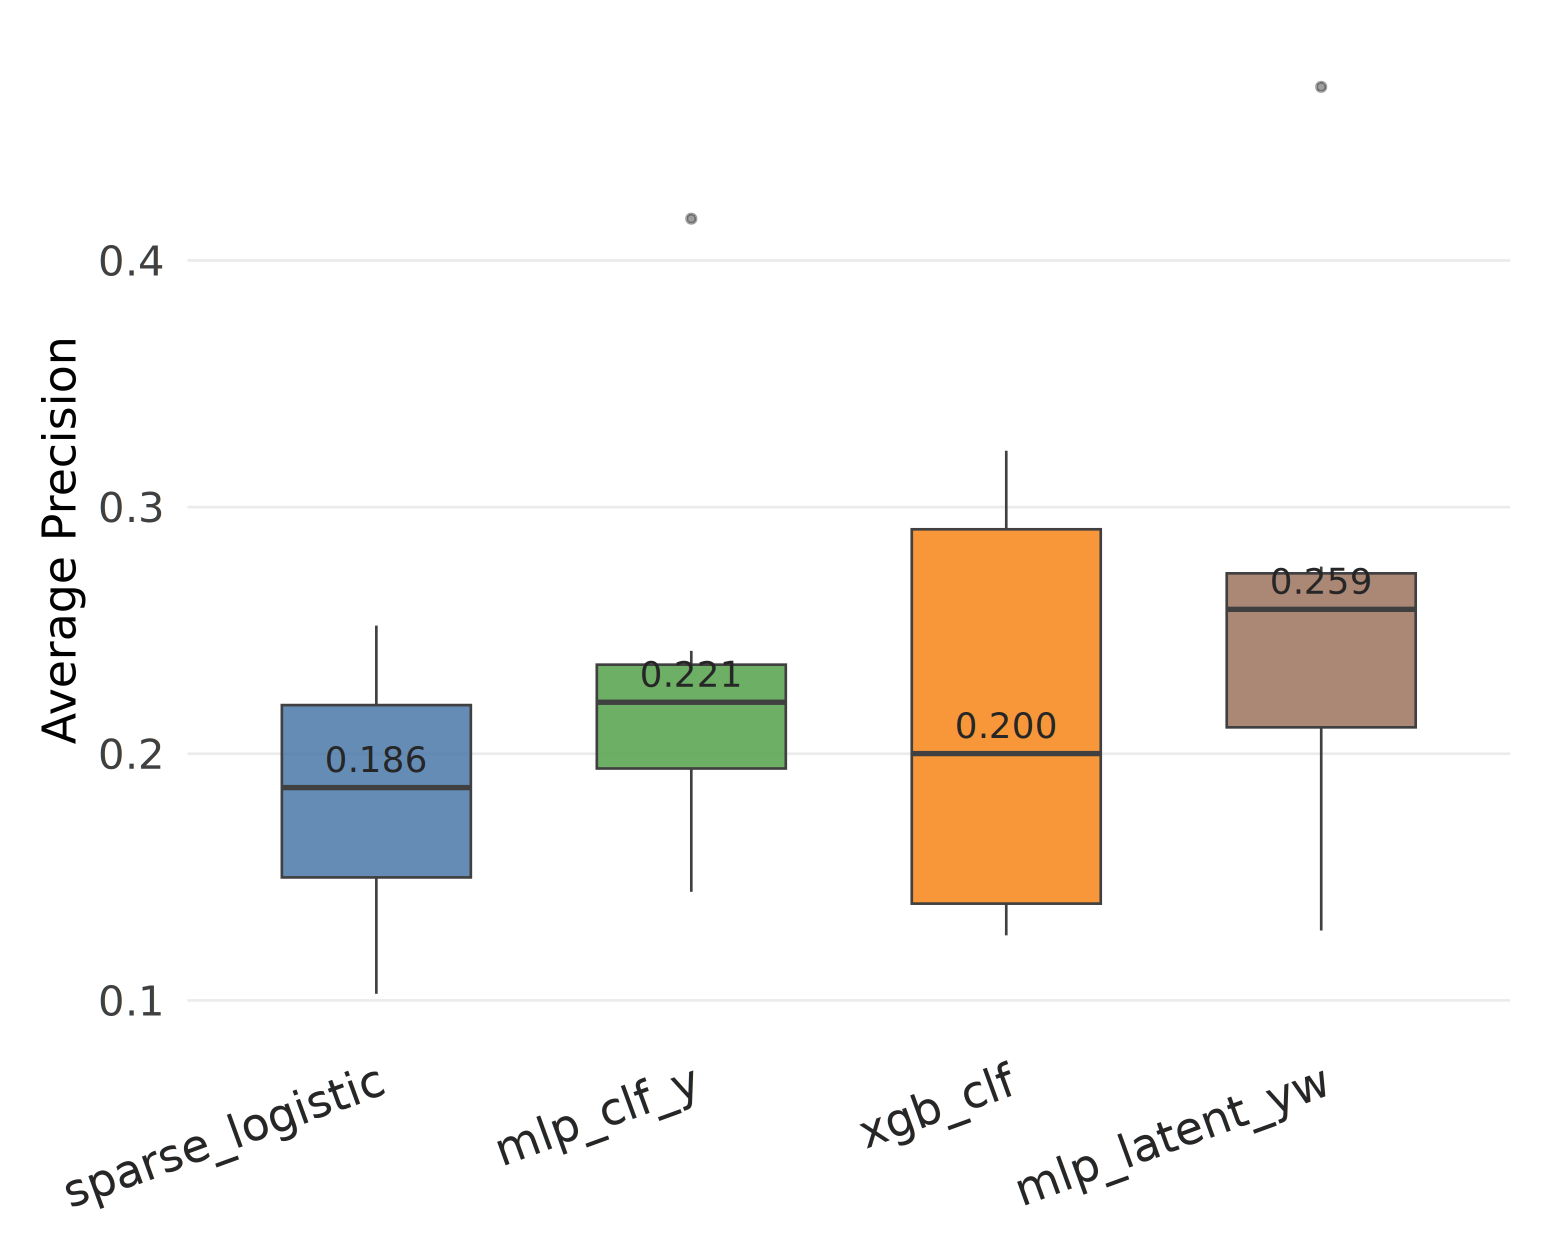
\includegraphics[width=\linewidth]{figures/fig_ap_y_ap_all_crc.png}
    \caption{CRC}
  \end{subfigure}\hfill
  \begin{subfigure}[t]{0.32\textwidth}
    \centering
    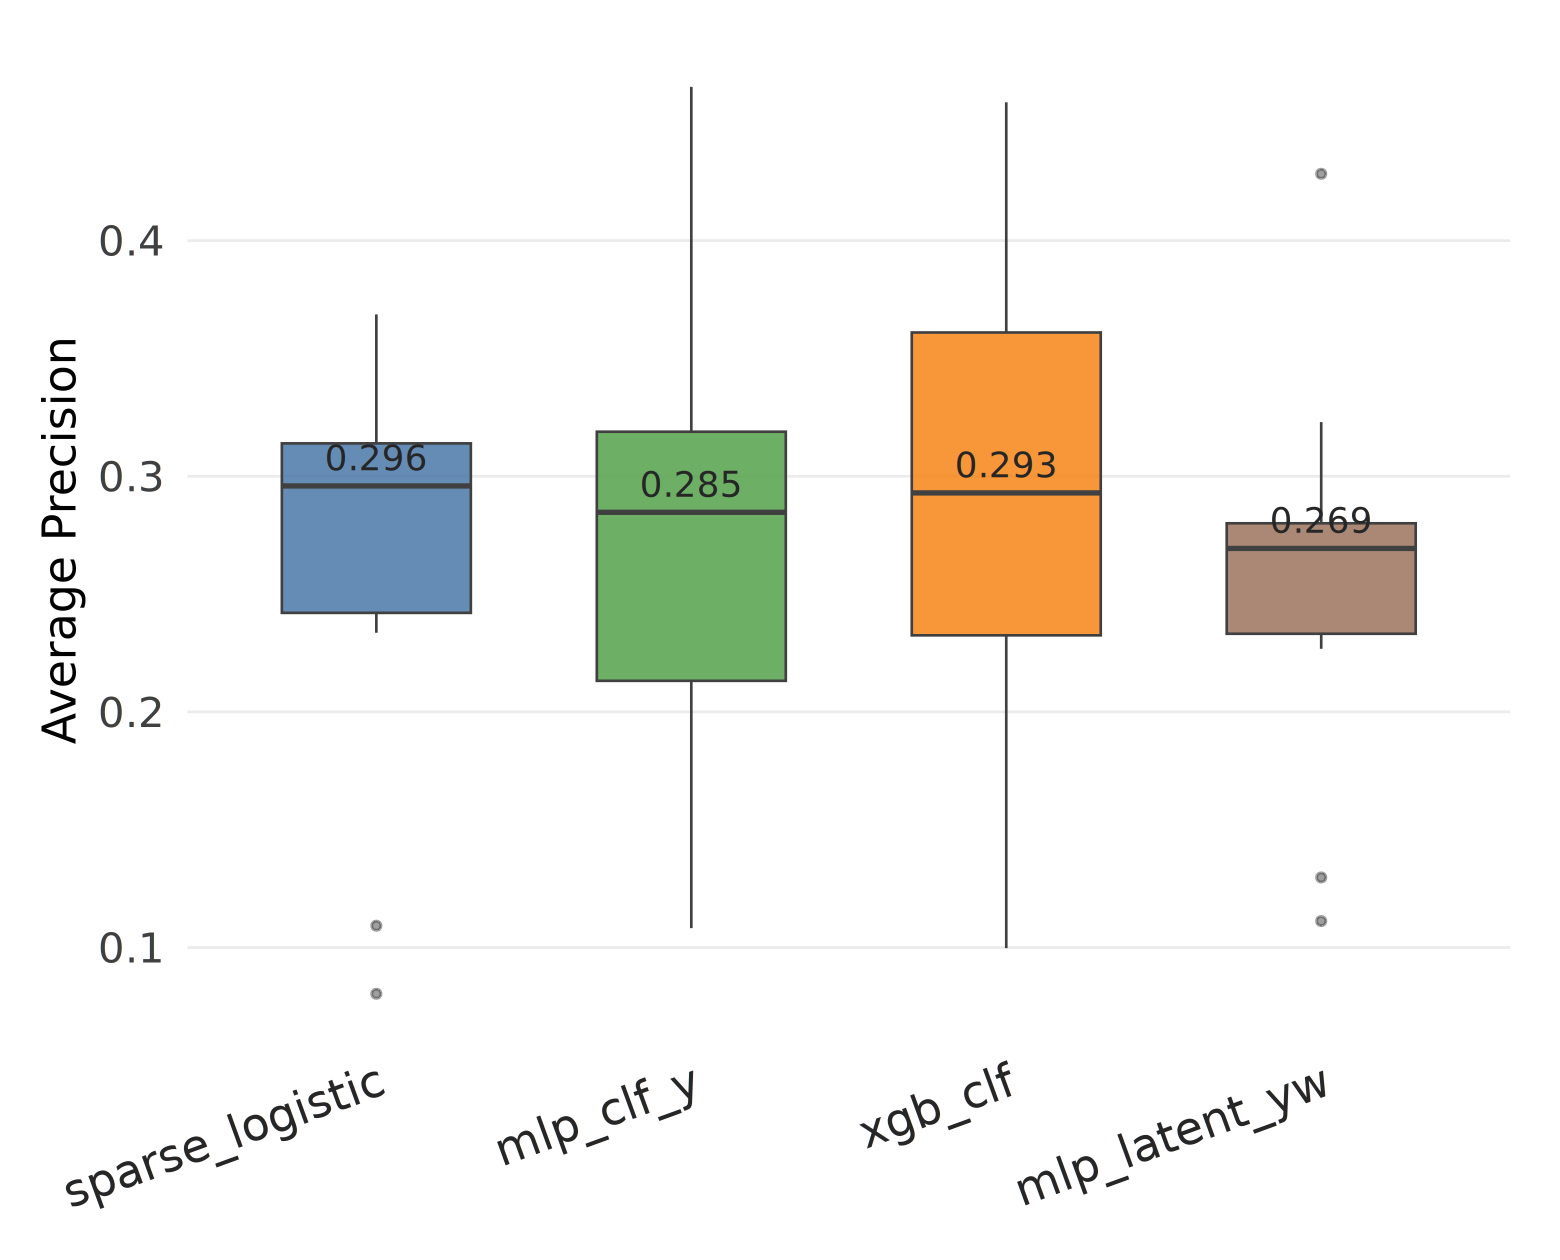
\includegraphics[width=\linewidth]{figures/fig_ap_y_ap_all_ibd.png}
    \caption{IBD}
  \end{subfigure}\hfill
  \begin{subfigure}[t]{0.32\textwidth}
    \centering
    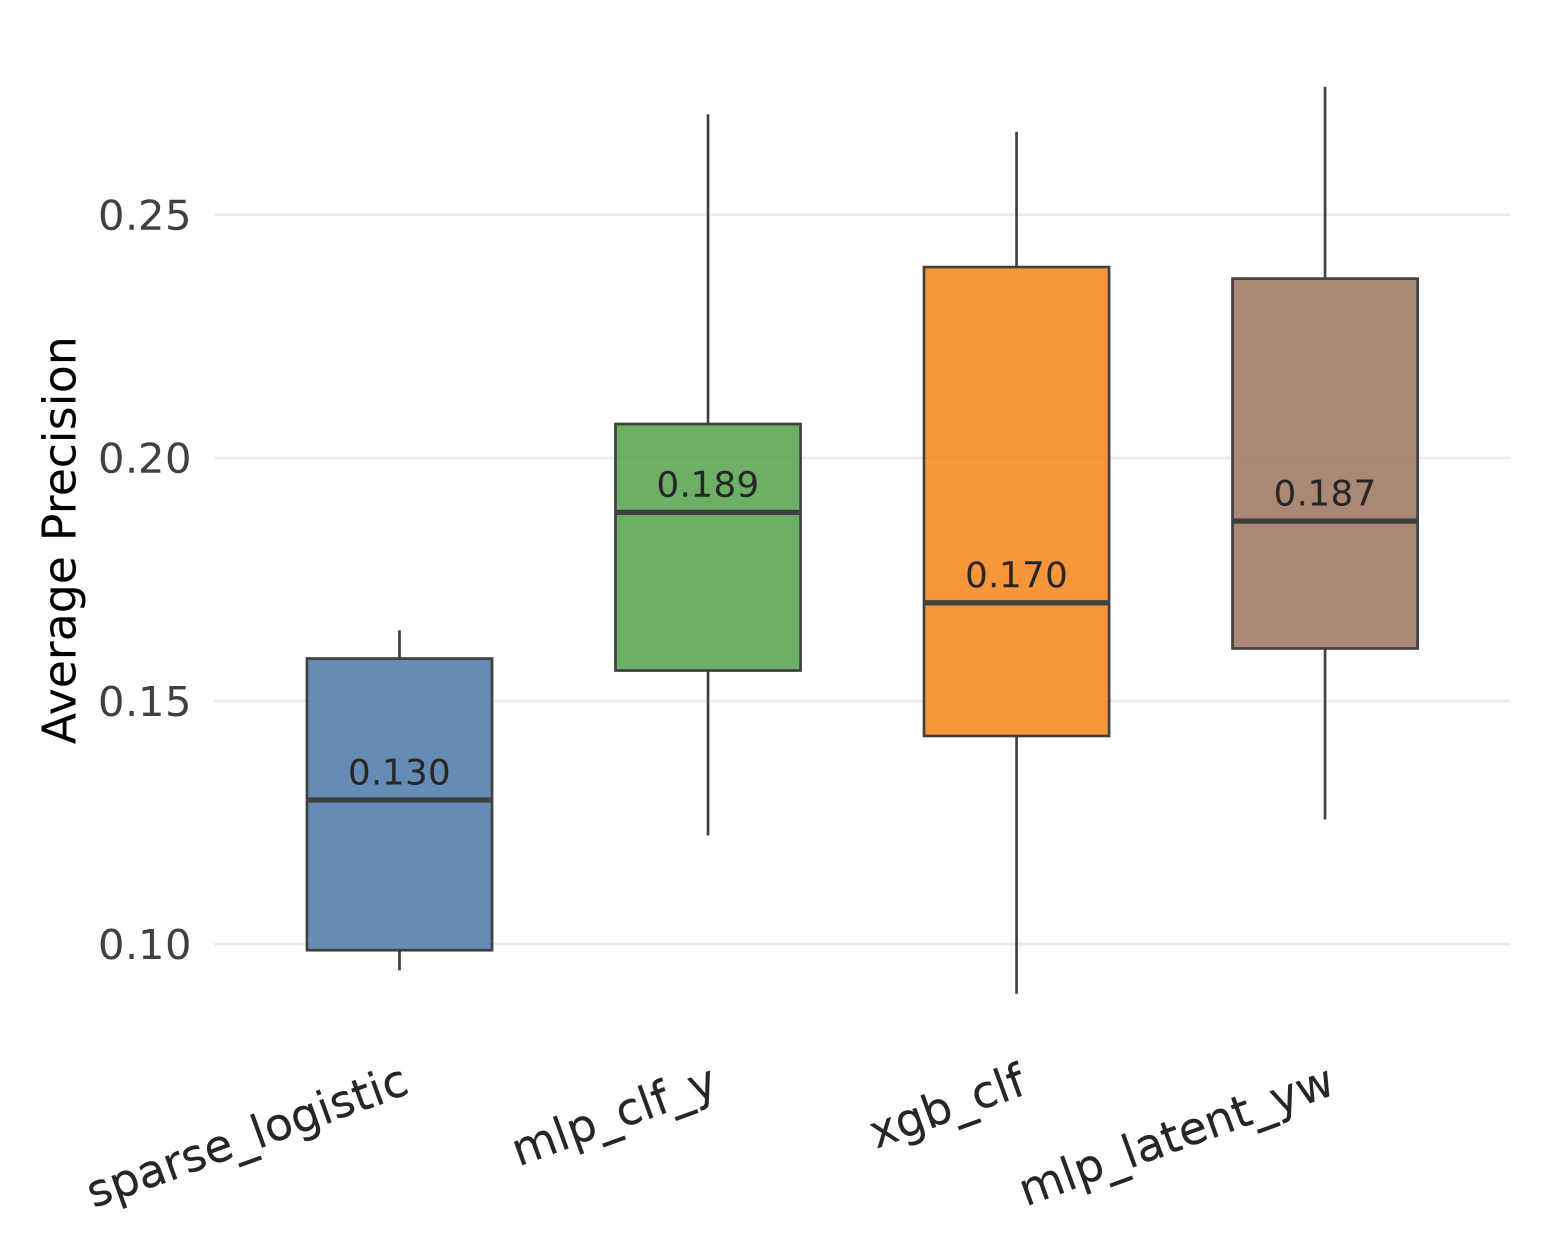
\includegraphics[width=\linewidth]{figures/fig_ap_y_ap_all_gvhd.png}
    \caption{GvHD}
  \end{subfigure}
  \caption{Test AP on CRISPR linkage, all models}
  \label{fig:ap-yapa}
\end{figure}

\begin{figure}[H]
  \centering
  \begin{subfigure}[t]{0.32\textwidth}
    \centering
    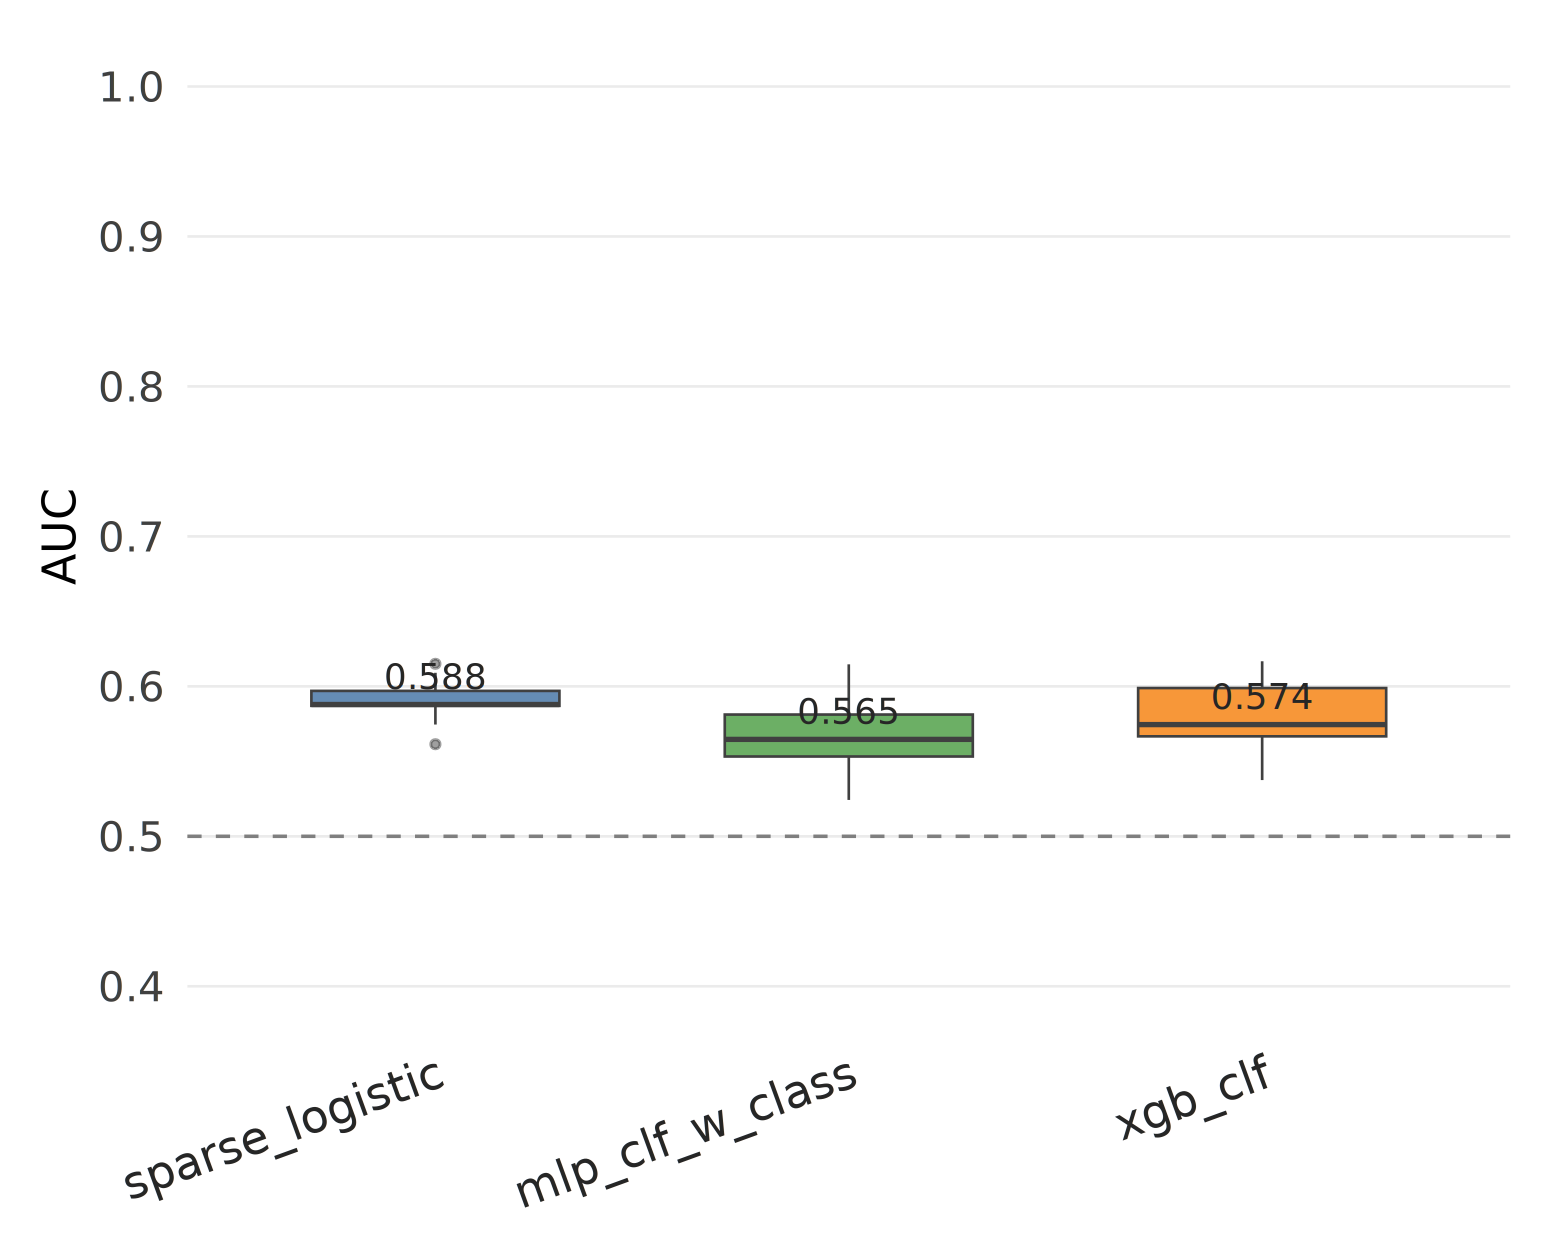
\includegraphics[width=\linewidth]{figures/fig_ap_w_class_auc_baseline_crc.png}
    \caption{CRC}
  \end{subfigure}\hfill
  \begin{subfigure}[t]{0.32\textwidth}
    \centering
    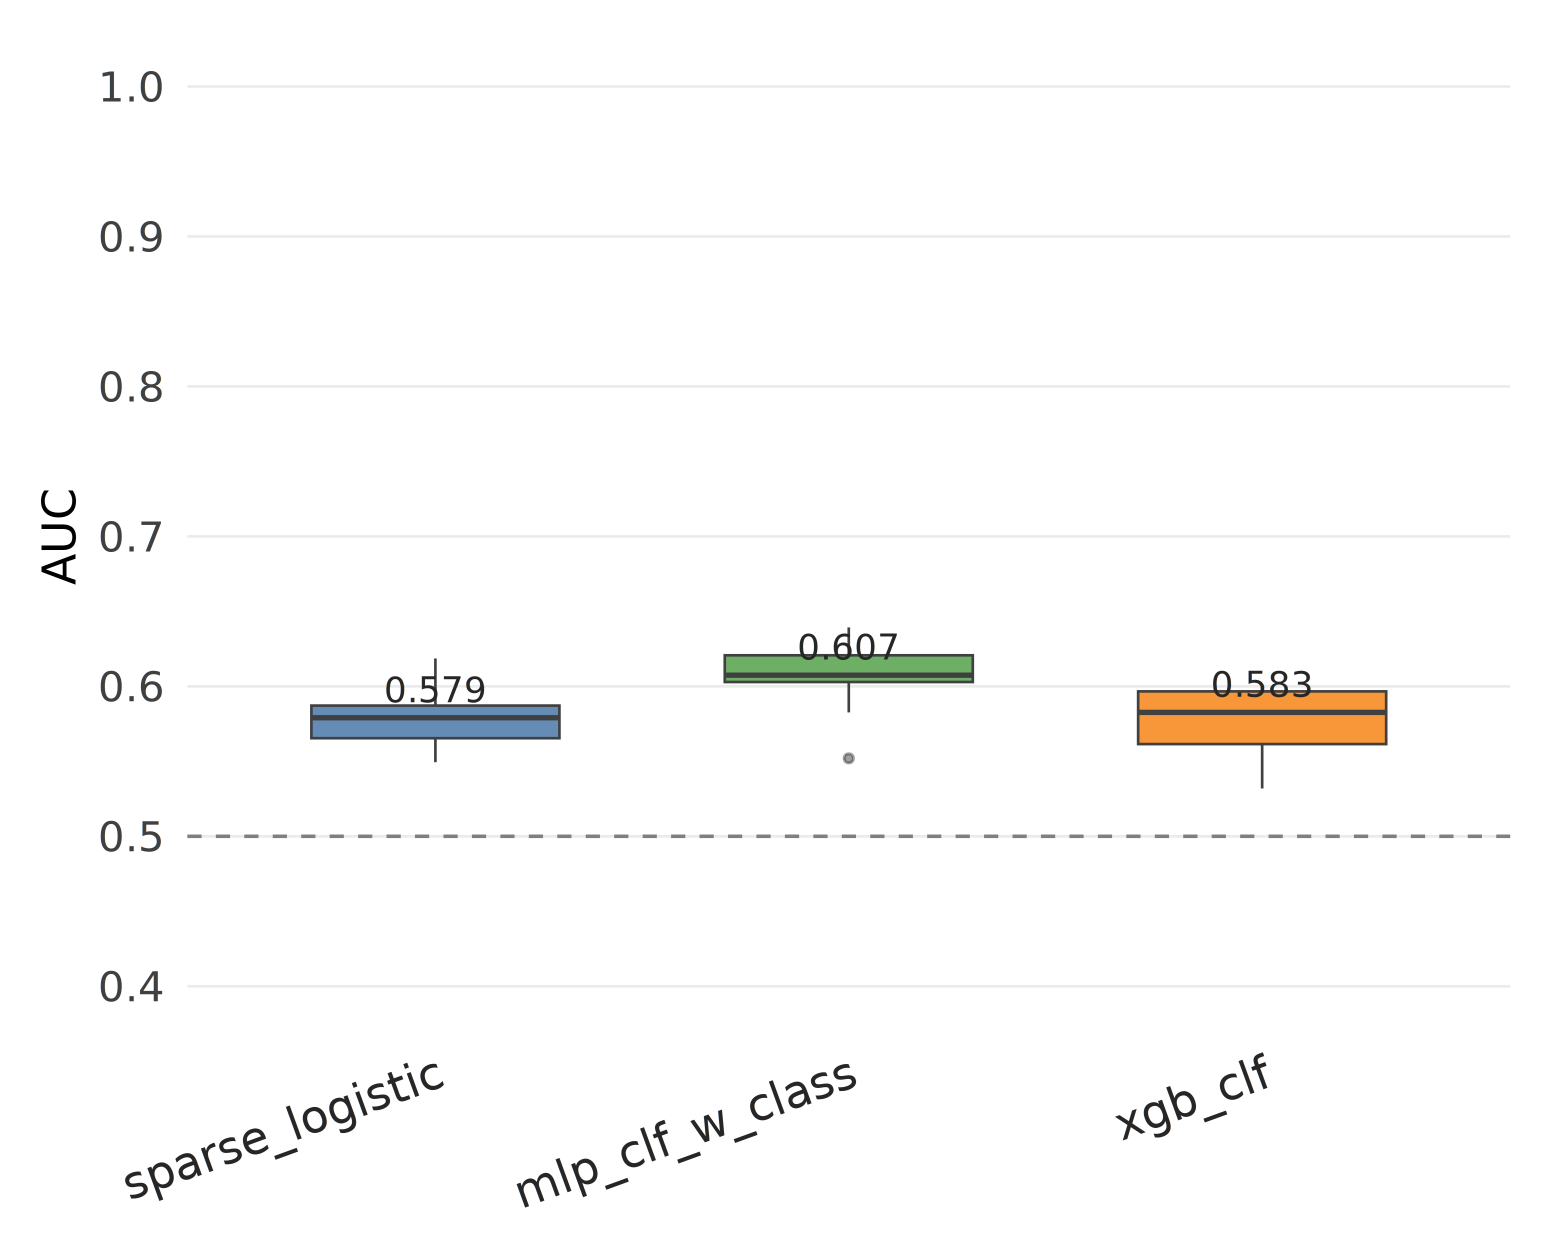
\includegraphics[width=\linewidth]{figures/fig_ap_w_class_auc_baseline_ibd.png}
    \caption{IBD}
  \end{subfigure}\hfill
  \begin{subfigure}[t]{0.32\textwidth}
    \centering
    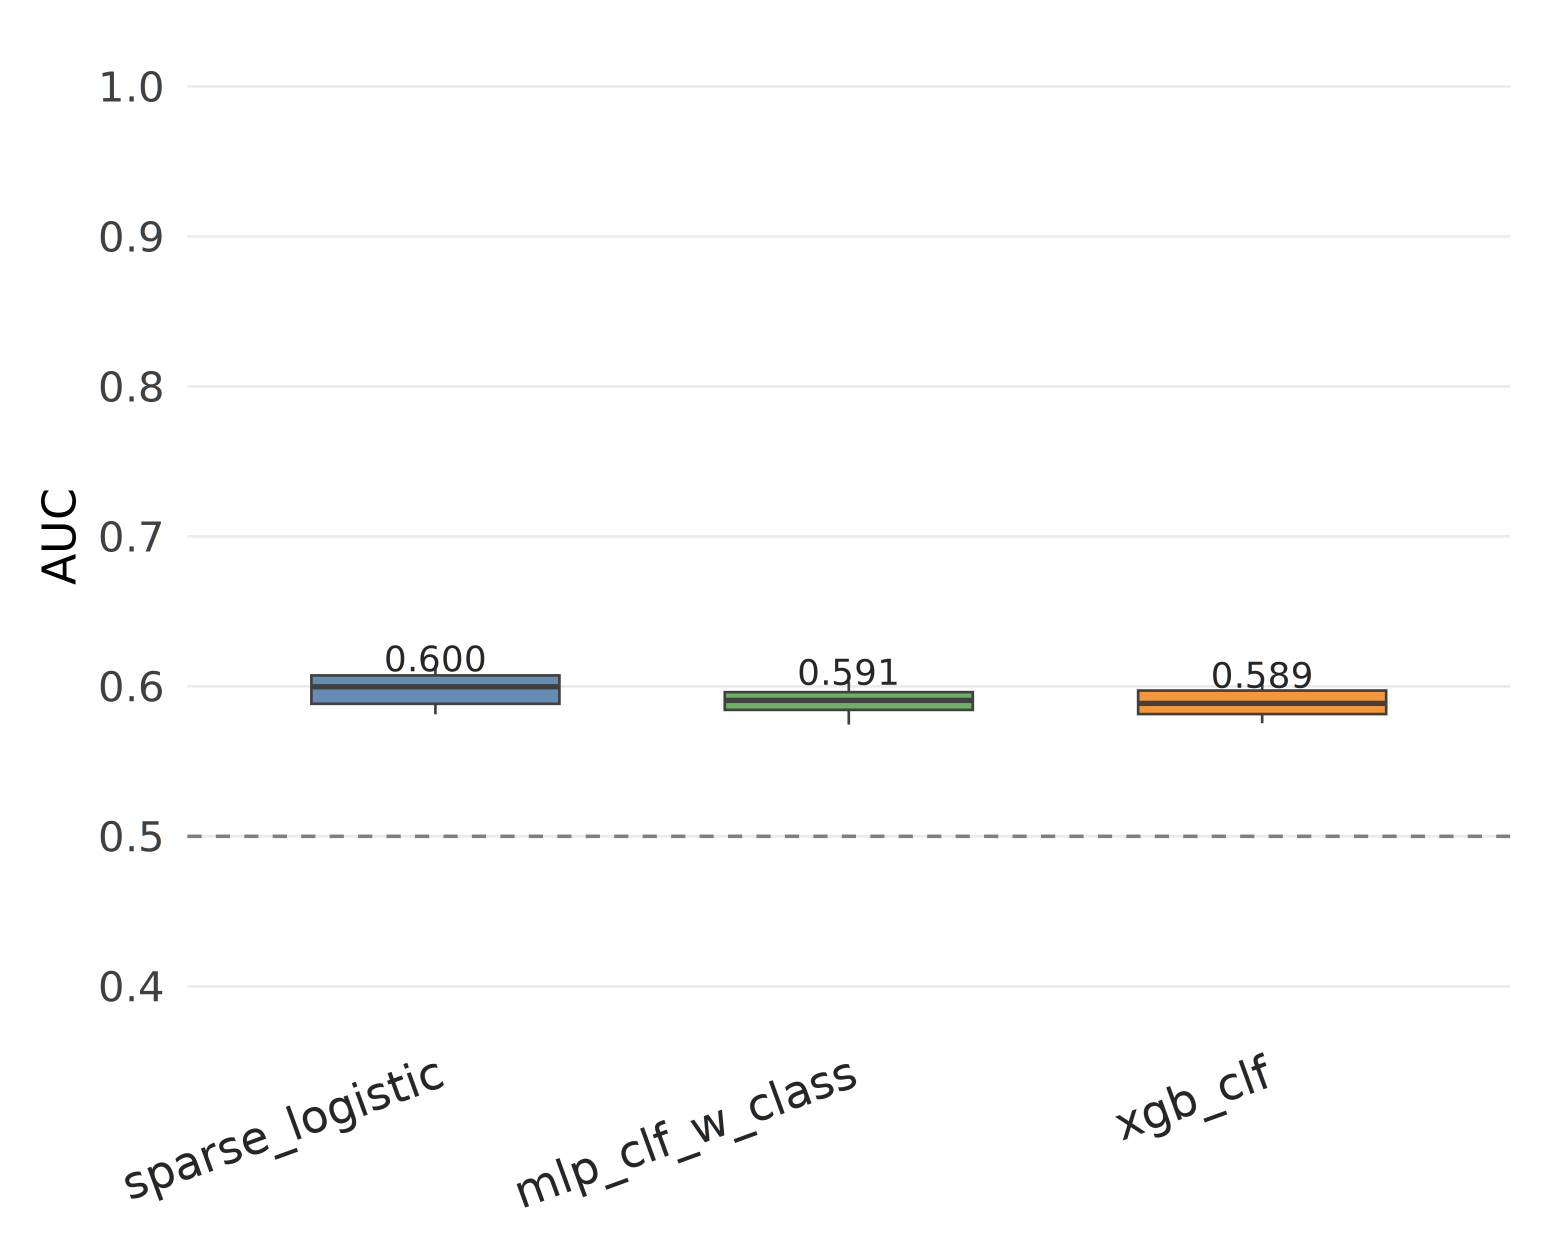
\includegraphics[width=\linewidth]{figures/fig_ap_w_class_auc_baseline_gvhd.png}
    \caption{GvHD}
  \end{subfigure}
  \caption{Test AUC on the binarised selection probability, baseline models}
  \label{fig:ap-wcaucb}
\end{figure}

\begin{figure}[H]
  \centering
  \begin{subfigure}[t]{0.32\textwidth}
    \centering
    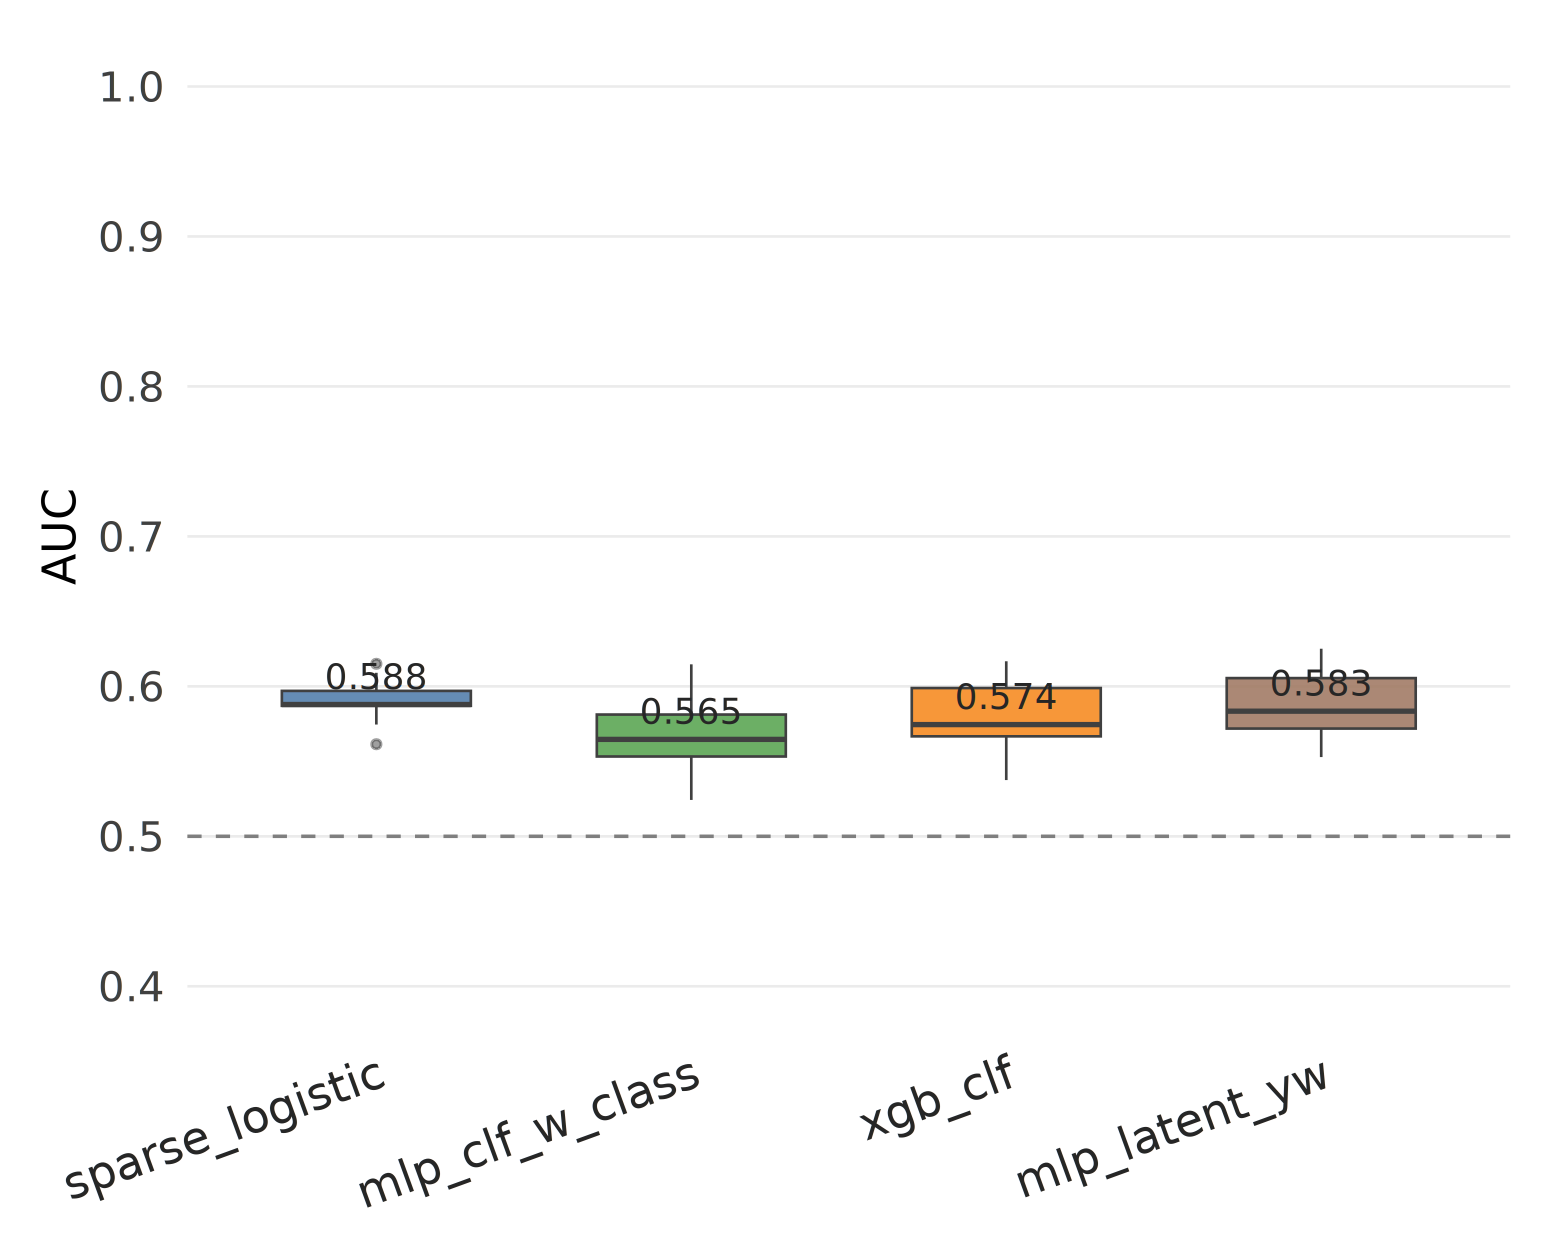
\includegraphics[width=\linewidth]{figures/fig_ap_w_class_auc_all_crc.png}
    \caption{CRC}
  \end{subfigure}\hfill
  \begin{subfigure}[t]{0.32\textwidth}
    \centering
    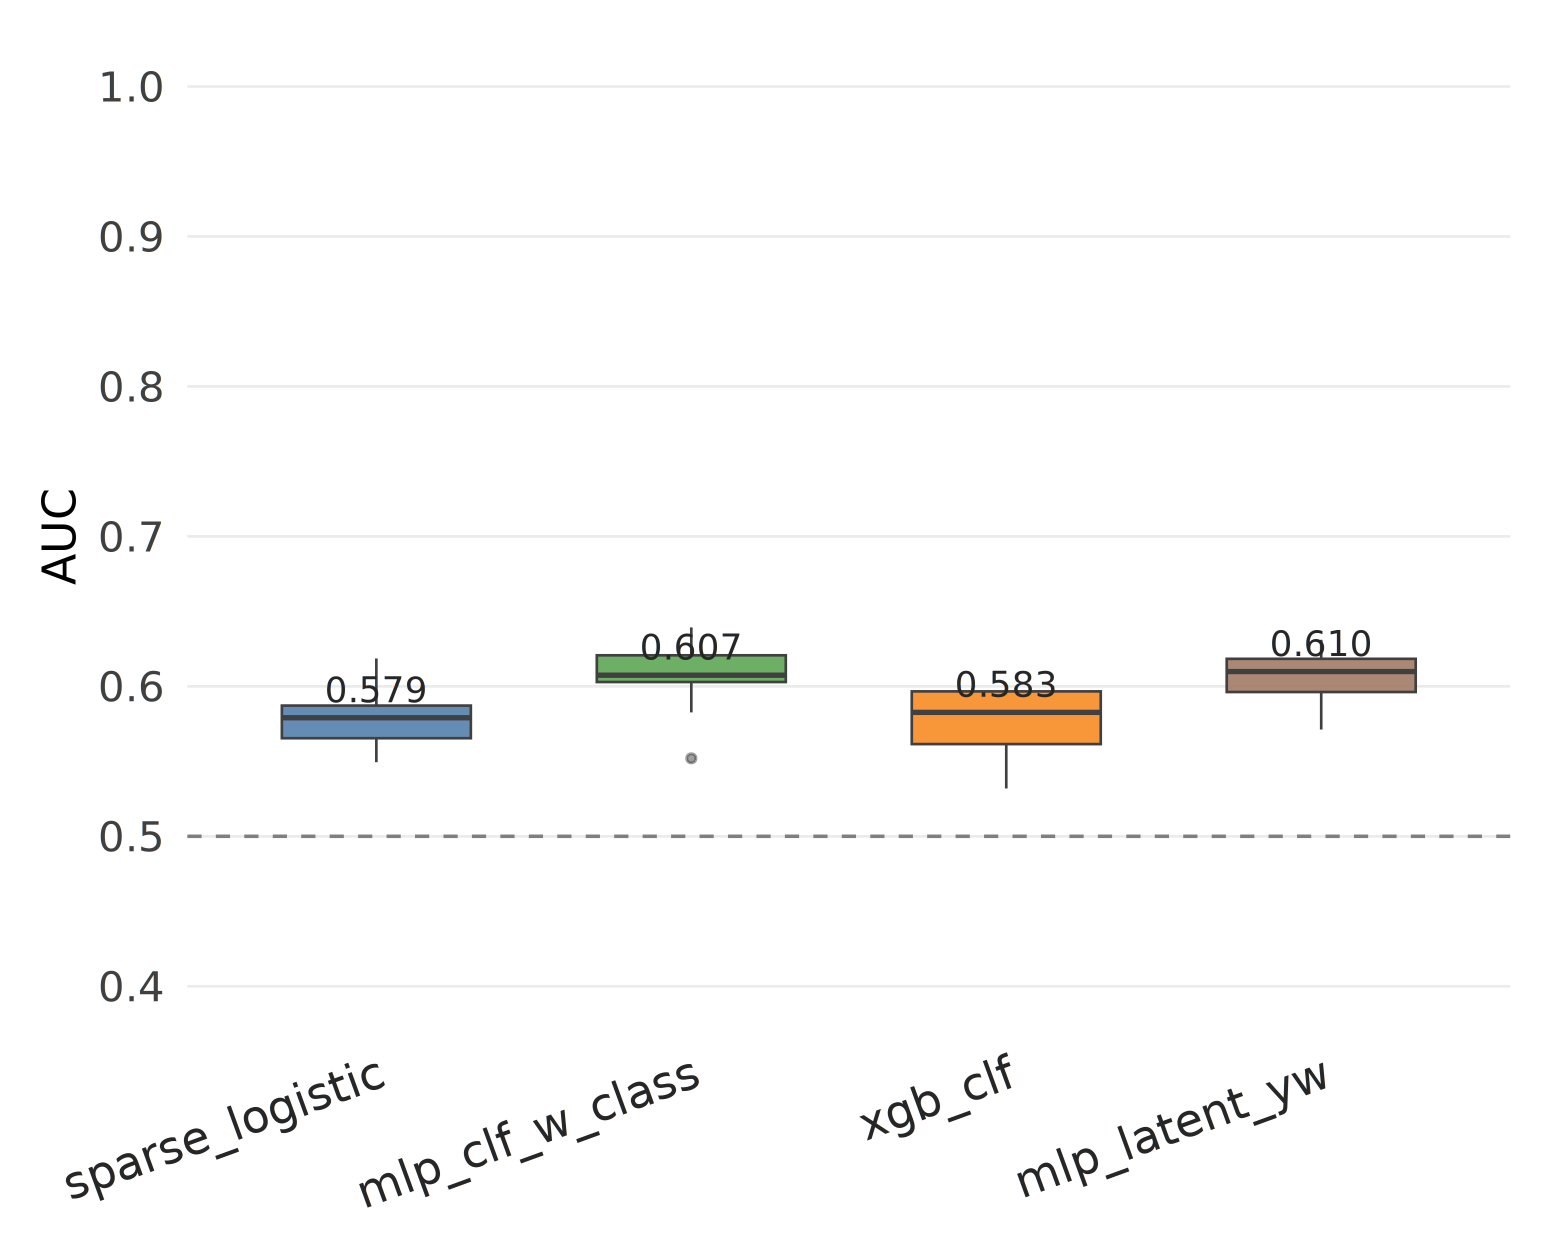
\includegraphics[width=\linewidth]{figures/fig_ap_w_class_auc_all_ibd.png}
    \caption{IBD}
  \end{subfigure}\hfill
  \begin{subfigure}[t]{0.32\textwidth}
    \centering
    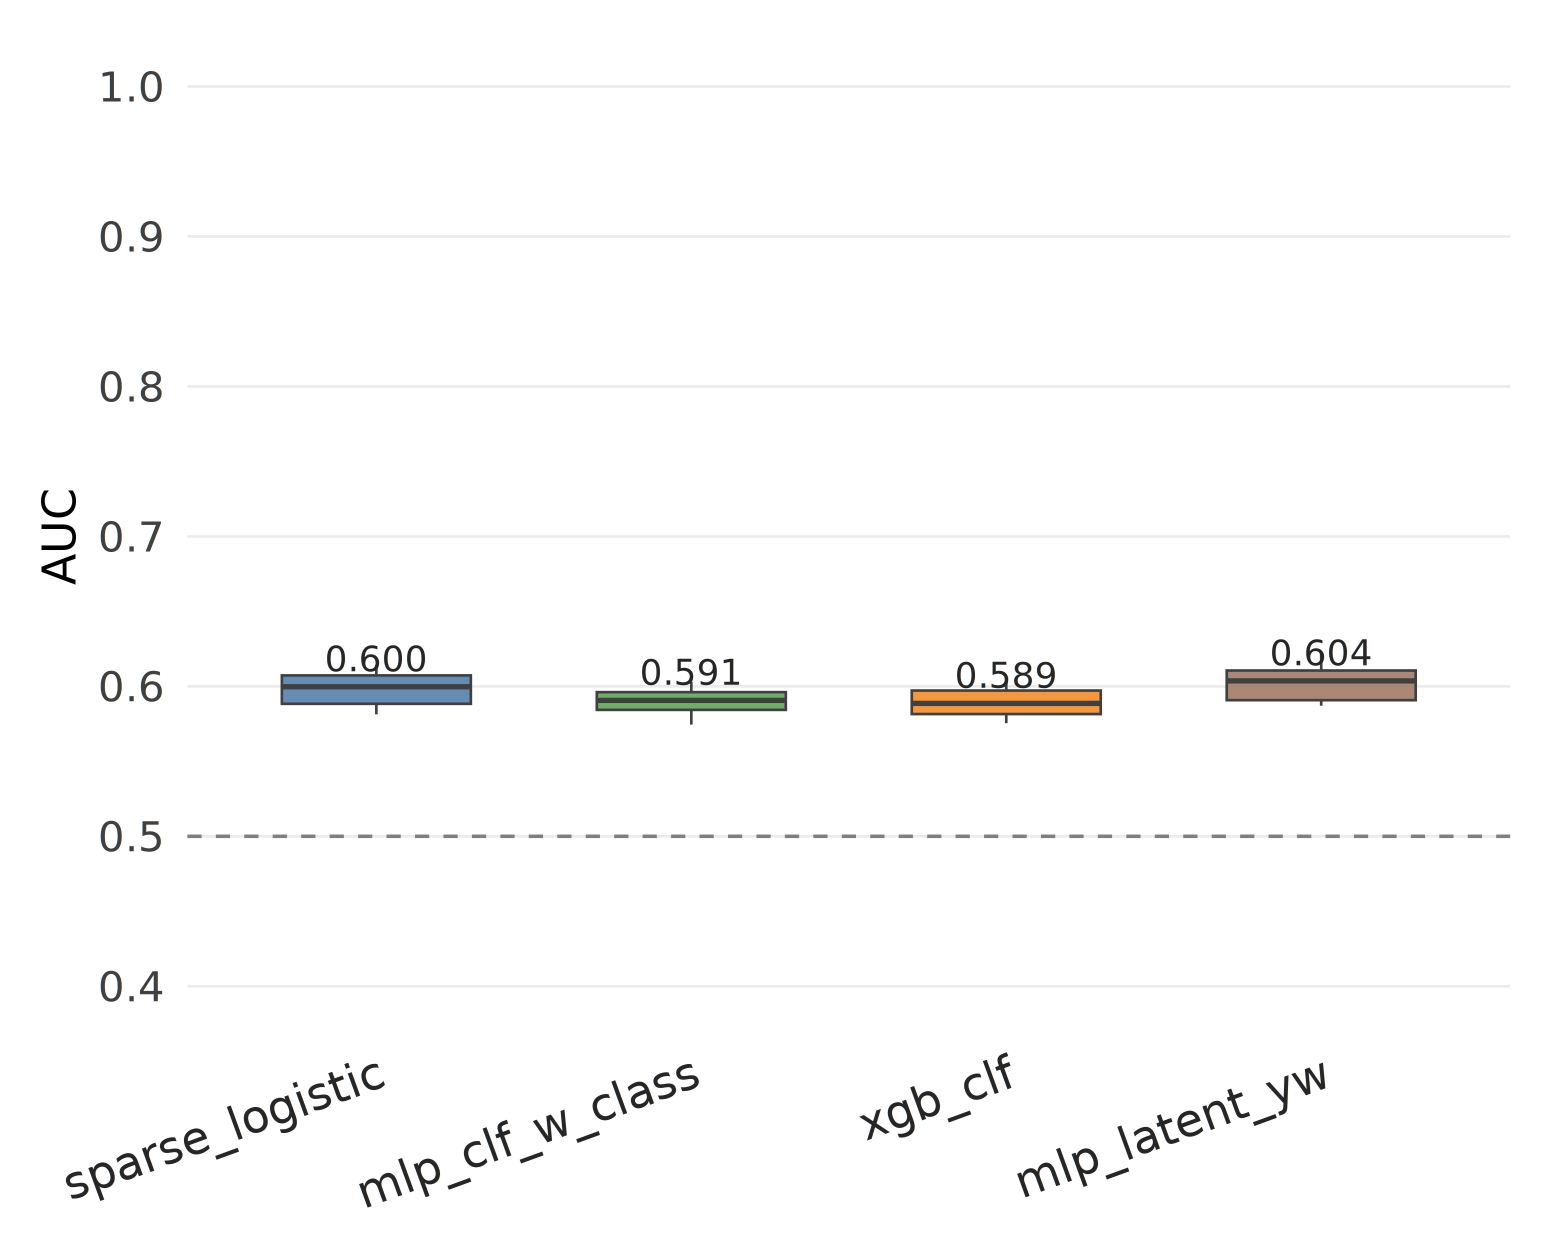
\includegraphics[width=\linewidth]{figures/fig_ap_w_class_auc_all_gvhd.png}
    \caption{GvHD}
  \end{subfigure}
  \caption{Test AUC on the binarised selection probability, all models}
  \label{fig:ap-wcauca}
\end{figure}

\begin{figure}[H]
  \centering
  \begin{subfigure}[t]{0.32\textwidth}
    \centering
    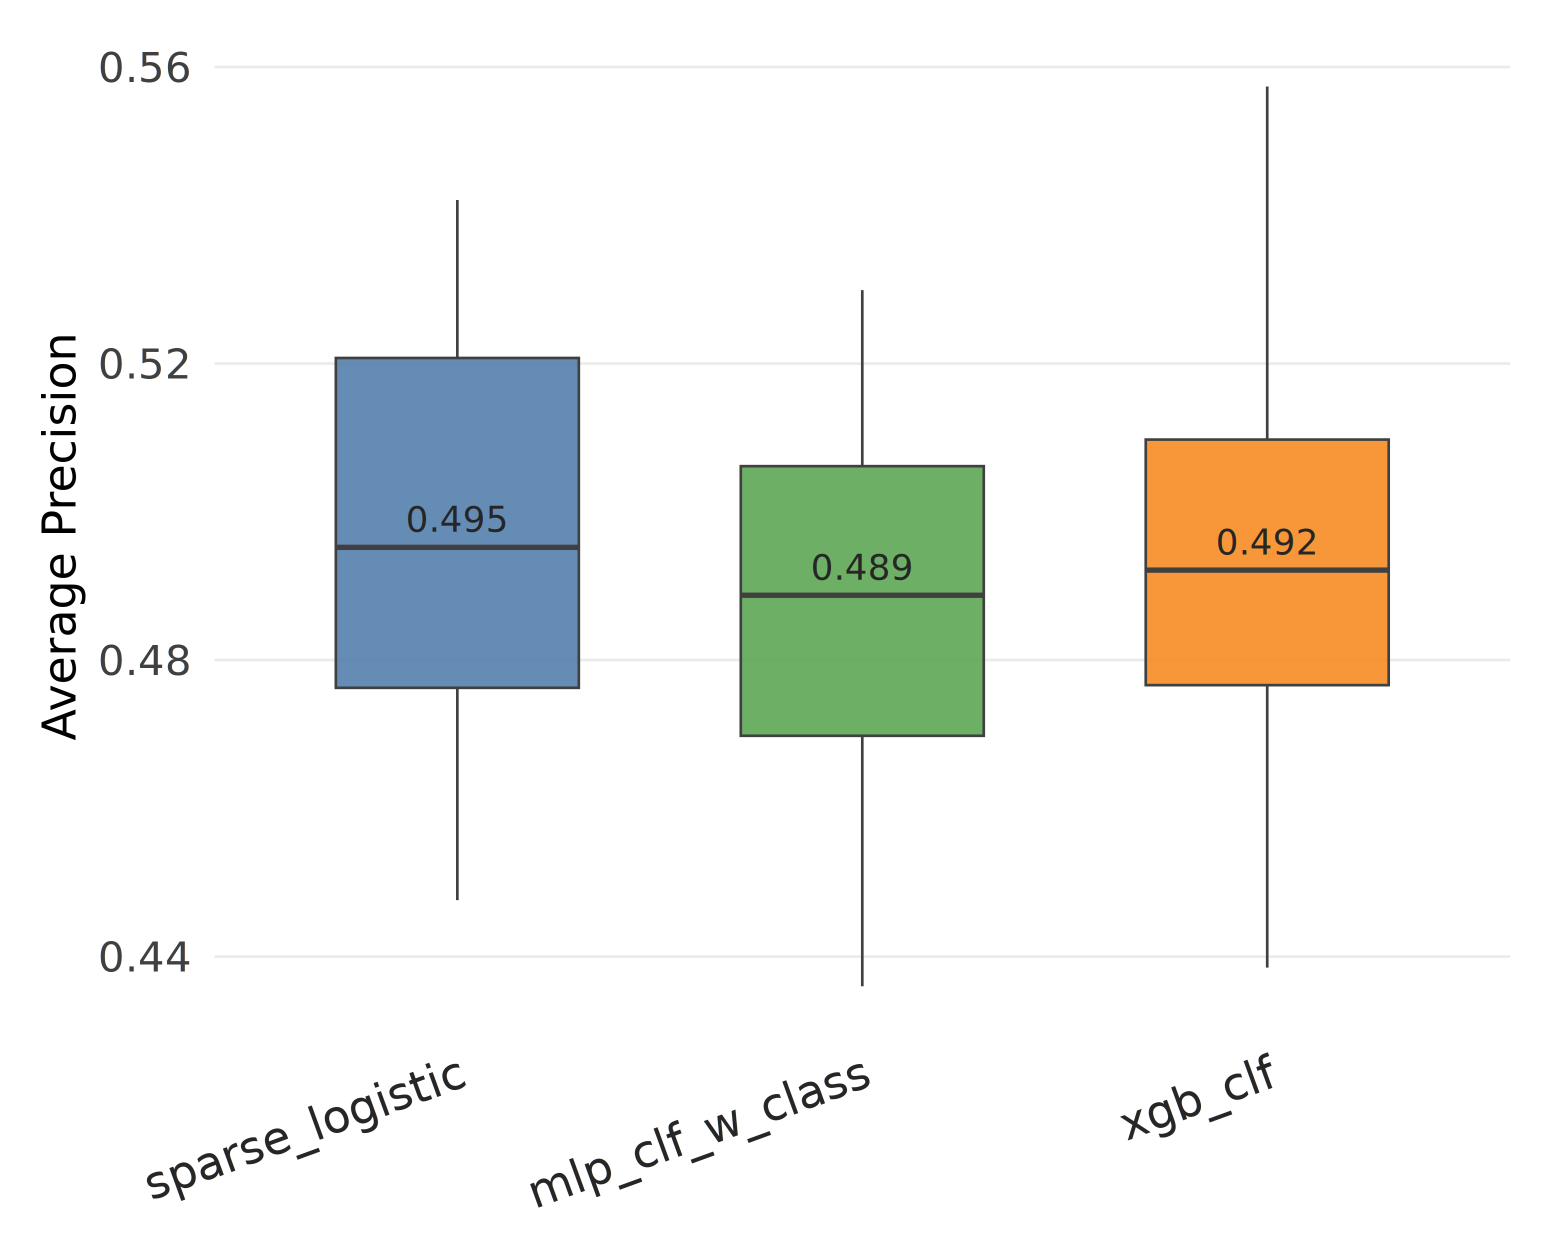
\includegraphics[width=\linewidth]{figures/fig_ap_w_class_ap_baseline_crc.png}
    \caption{CRC}
  \end{subfigure}\hfill
  \begin{subfigure}[t]{0.32\textwidth}
    \centering
    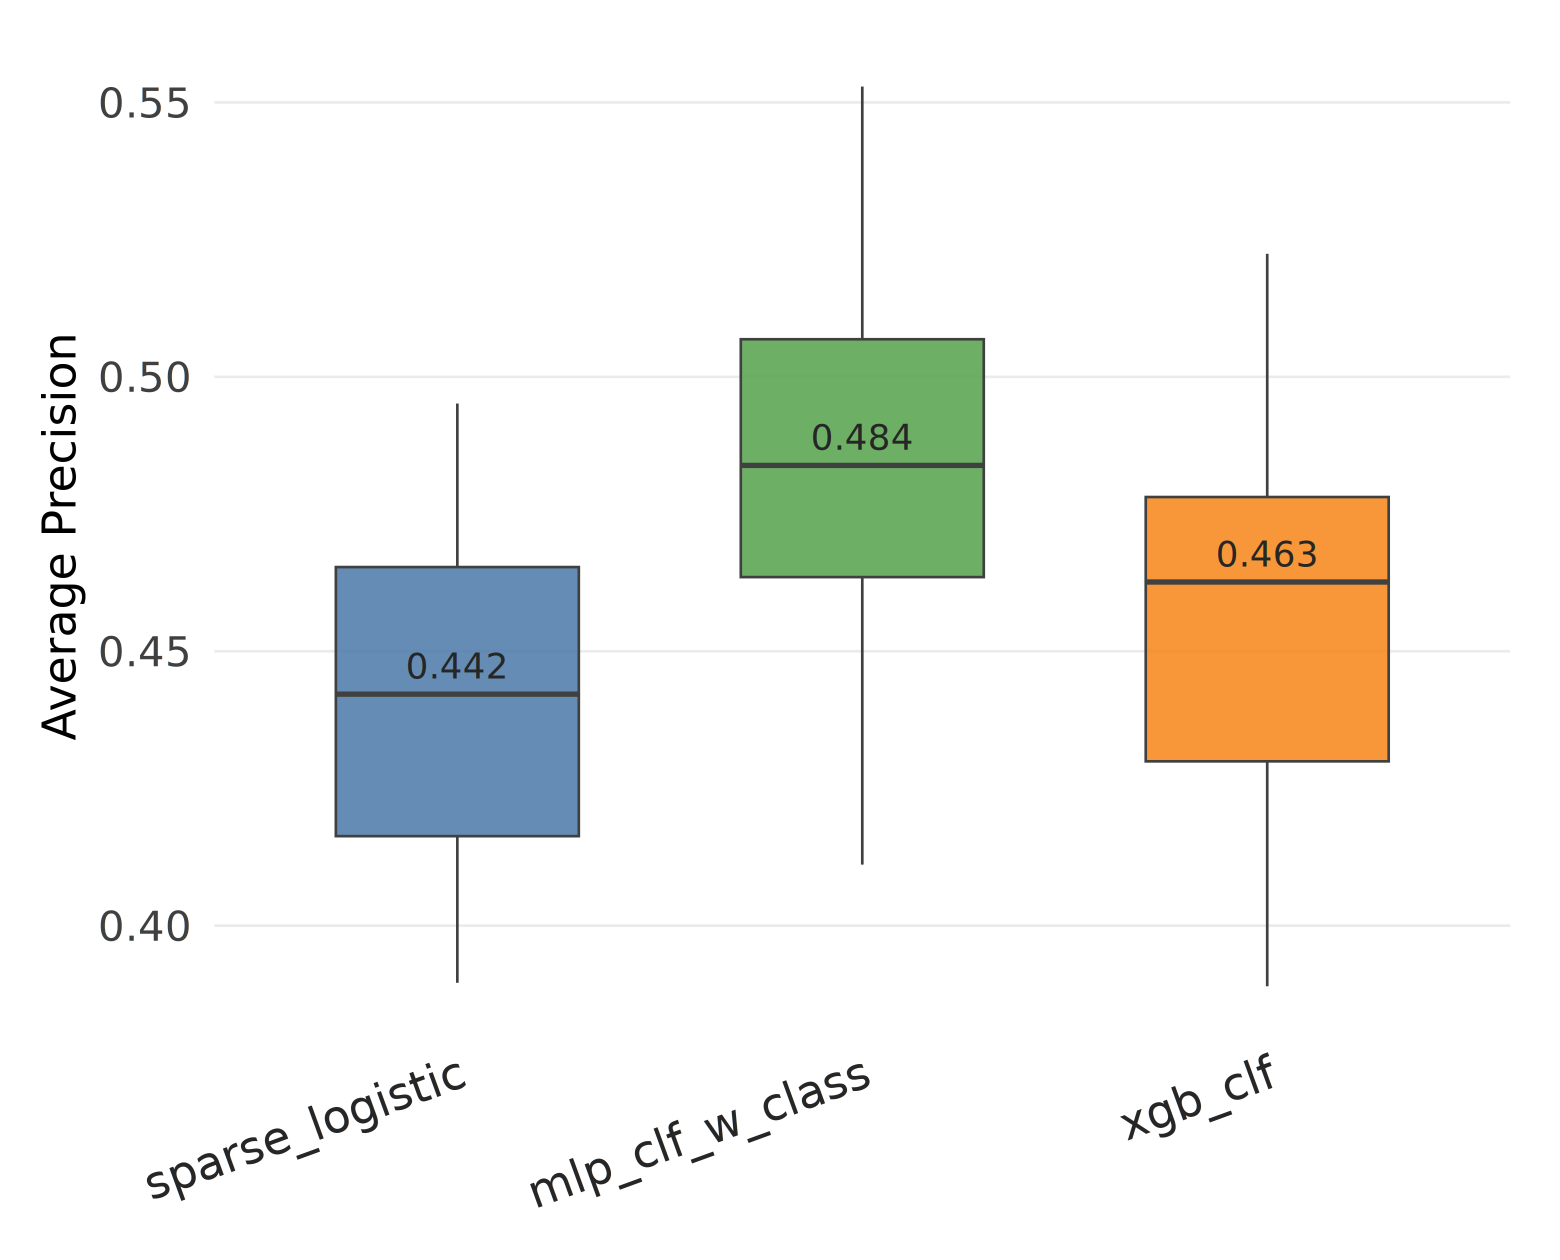
\includegraphics[width=\linewidth]{figures/fig_ap_w_class_ap_baseline_ibd.png}
    \caption{IBD}
  \end{subfigure}\hfill
  \begin{subfigure}[t]{0.32\textwidth}
    \centering
    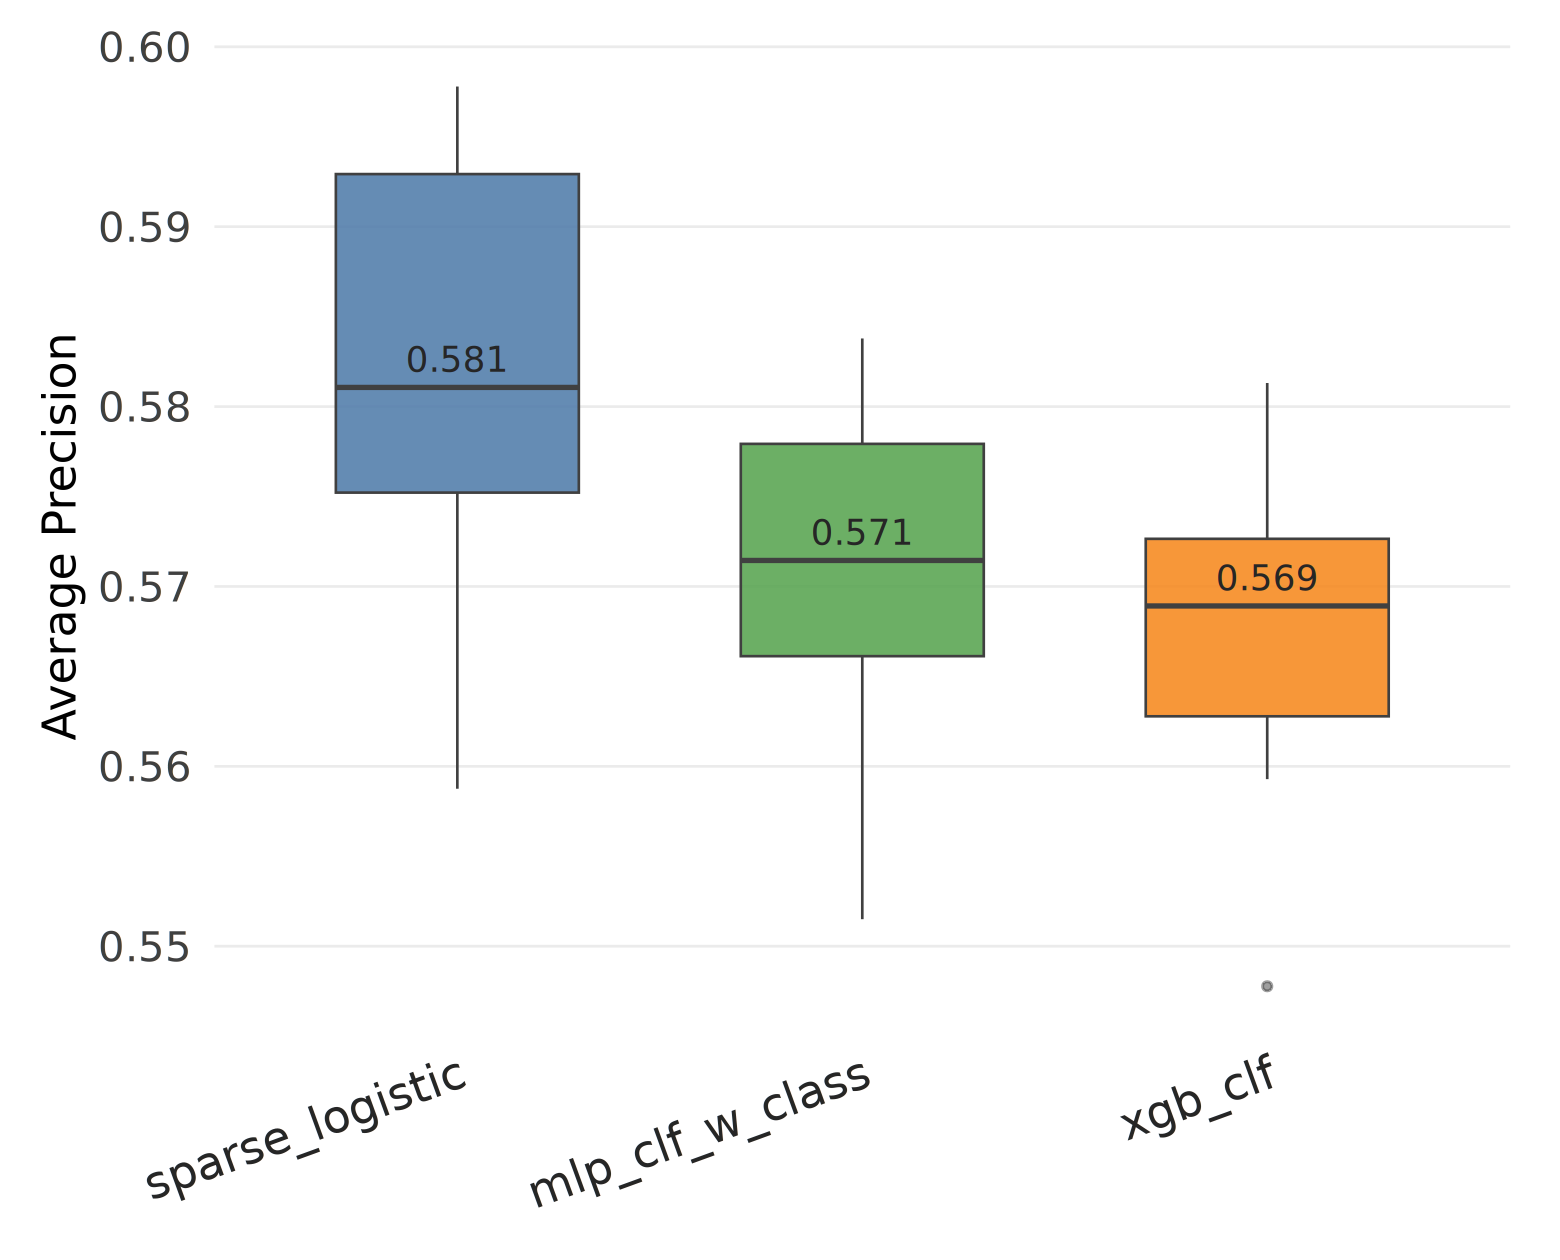
\includegraphics[width=\linewidth]{figures/fig_ap_w_class_ap_baseline_gvhd.png}
    \caption{GvHD}
  \end{subfigure}
  \caption{Test AP on the binarised selection probability, baseline models}
  \label{fig:ap-wcapb}
\end{figure}

\begin{figure}[H]
  \centering
  \begin{subfigure}[t]{0.32\textwidth}
    \centering
    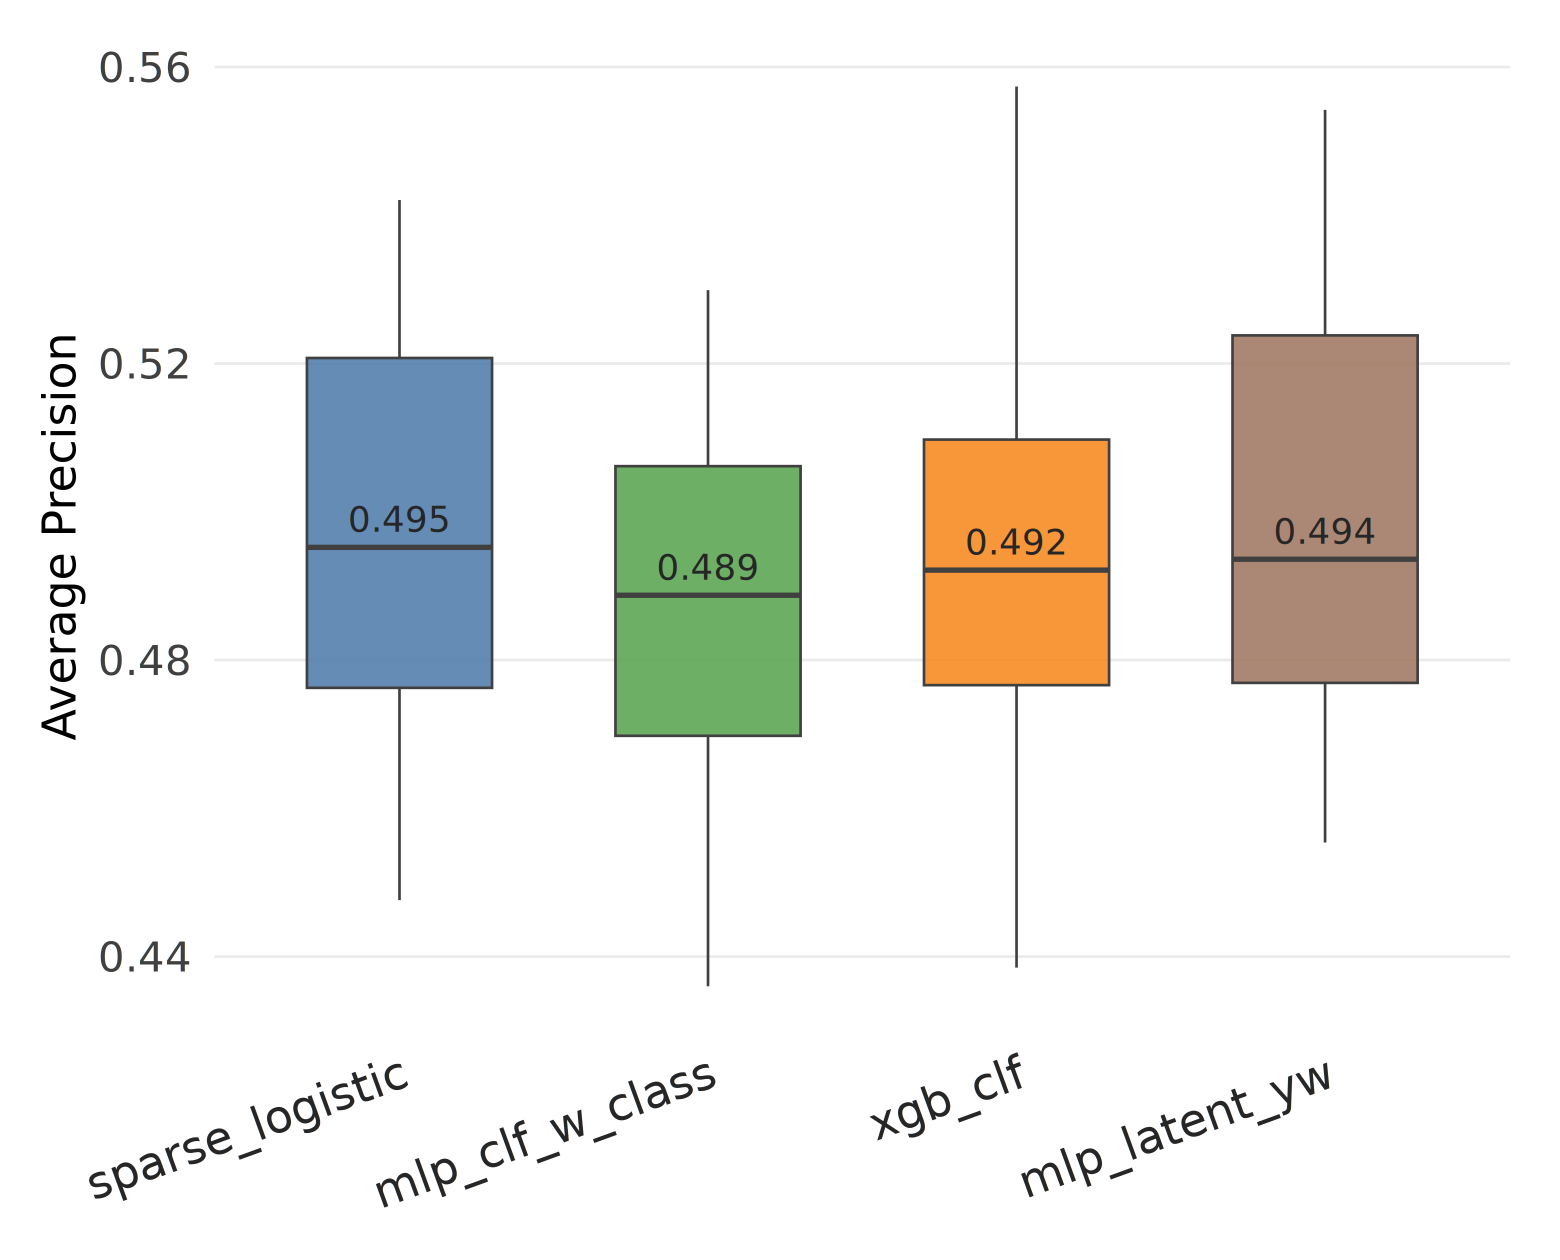
\includegraphics[width=\linewidth]{figures/fig_ap_w_class_ap_all_crc.png}
    \caption{CRC}
  \end{subfigure}\hfill
  \begin{subfigure}[t]{0.32\textwidth}
    \centering
    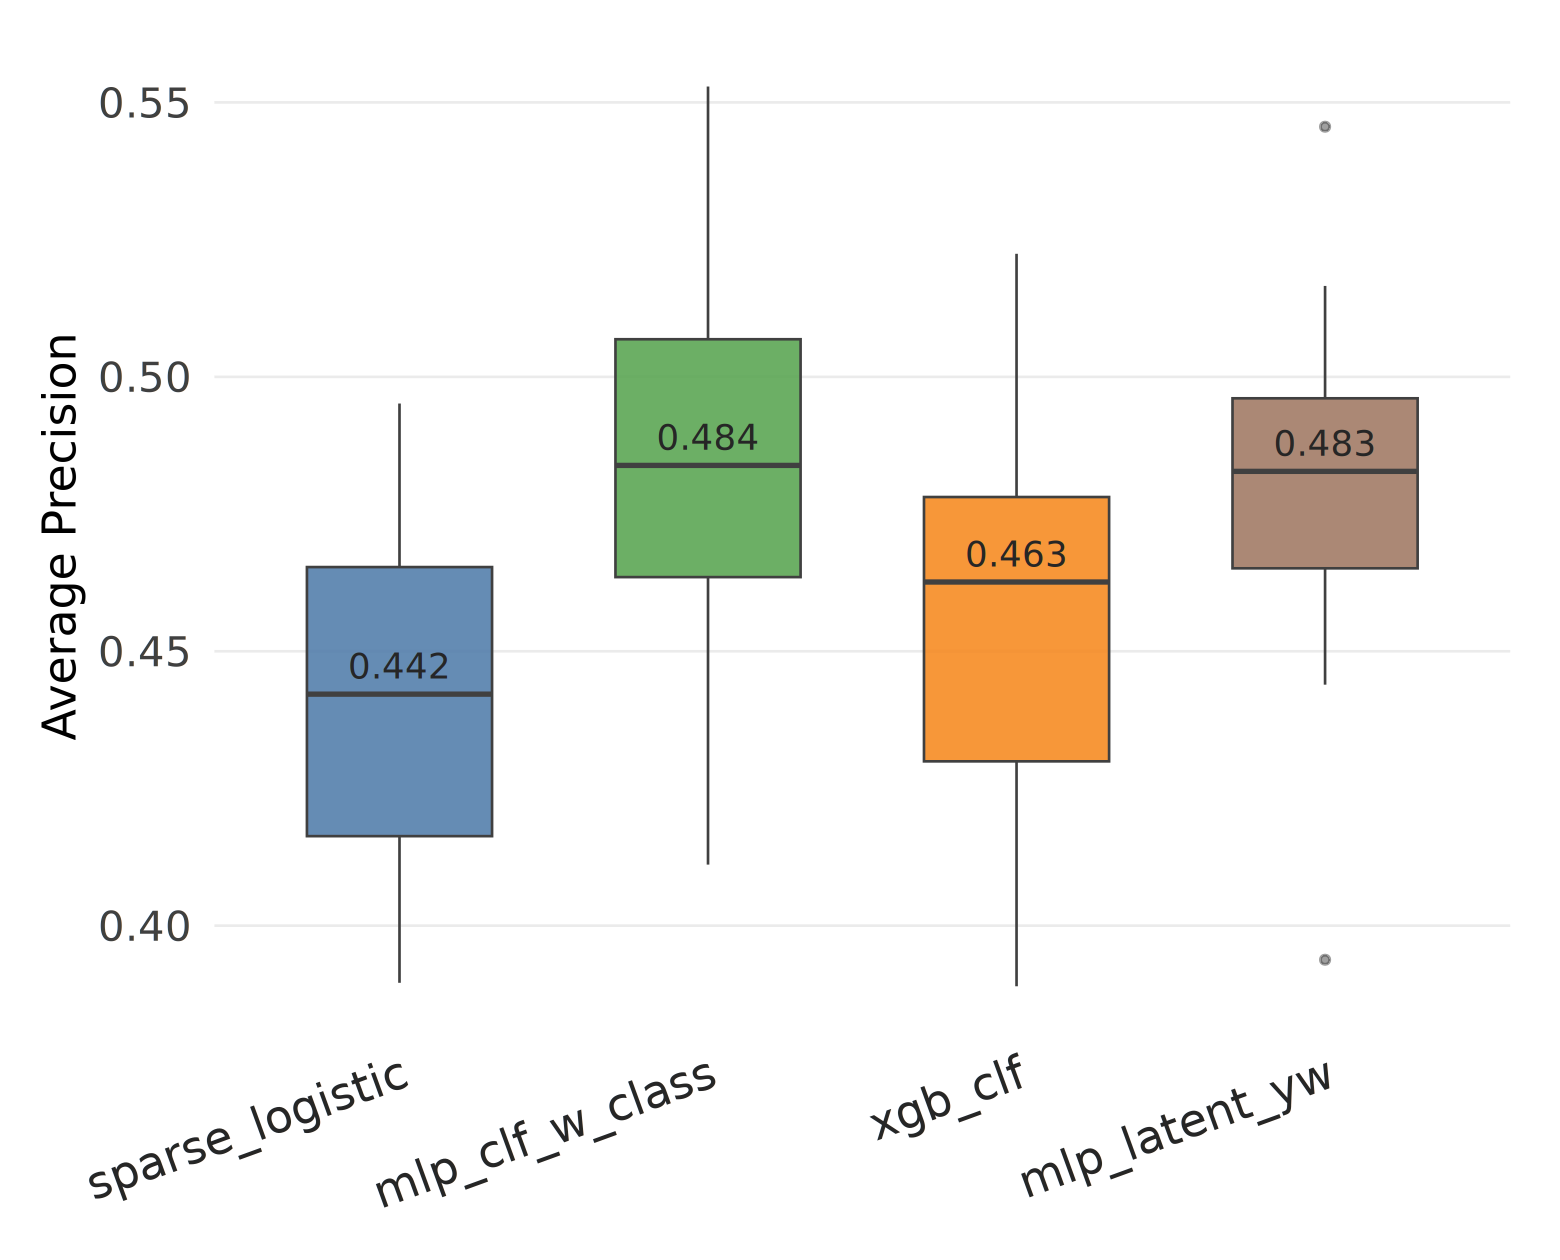
\includegraphics[width=\linewidth]{figures/fig_ap_w_class_ap_all_ibd.png}
    \caption{IBD}
  \end{subfigure}\hfill
  \begin{subfigure}[t]{0.32\textwidth}
    \centering
    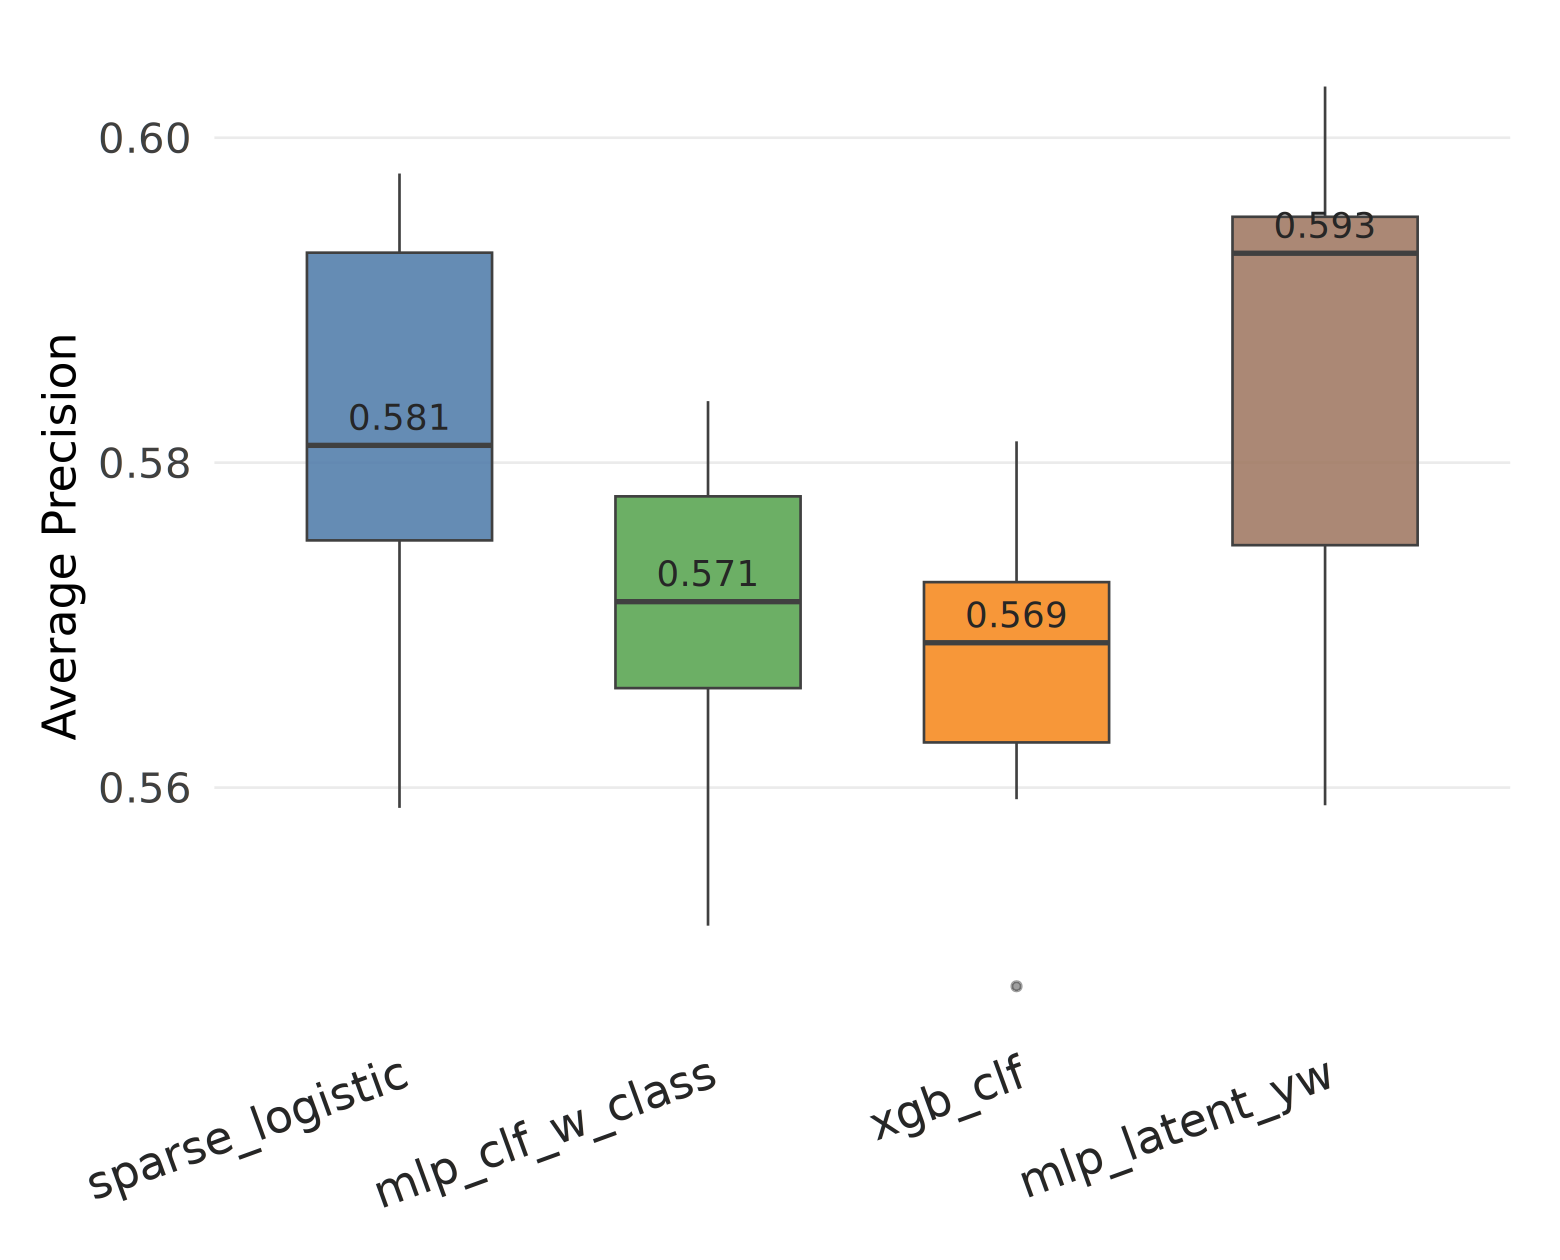
\includegraphics[width=\linewidth]{figures/fig_ap_w_class_ap_all_gvhd.png}
    \caption{GvHD}
  \end{subfigure}
  \caption{Test AP on the binarised selection probability, all models}
  \label{fig:ap-wcapa}
\end{figure}

\begin{figure}[H]
  \centering
  \begin{subfigure}[t]{0.32\textwidth}
    \centering
    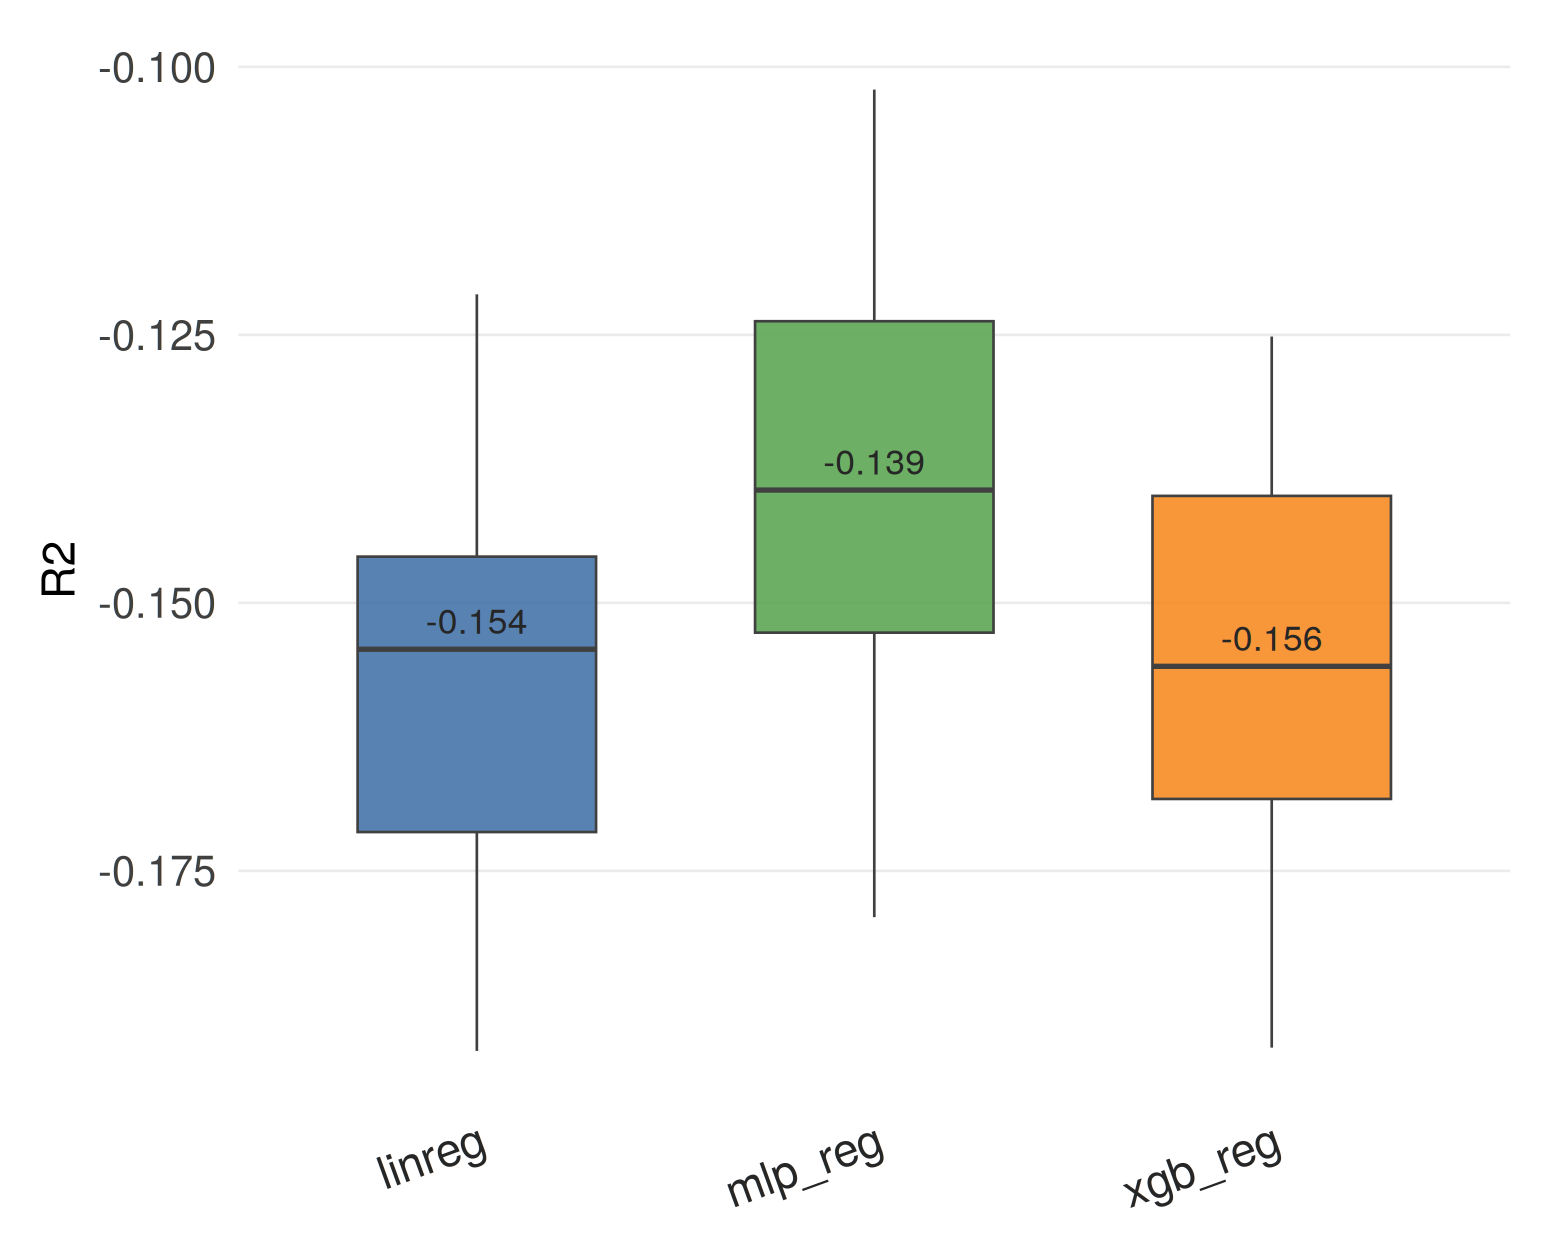
\includegraphics[width=\linewidth]{figures/fig_ap_w_reg_r2_baseline_crc.png}
    \caption{CRC}
  \end{subfigure}\hfill
  \begin{subfigure}[t]{0.32\textwidth}
    \centering
    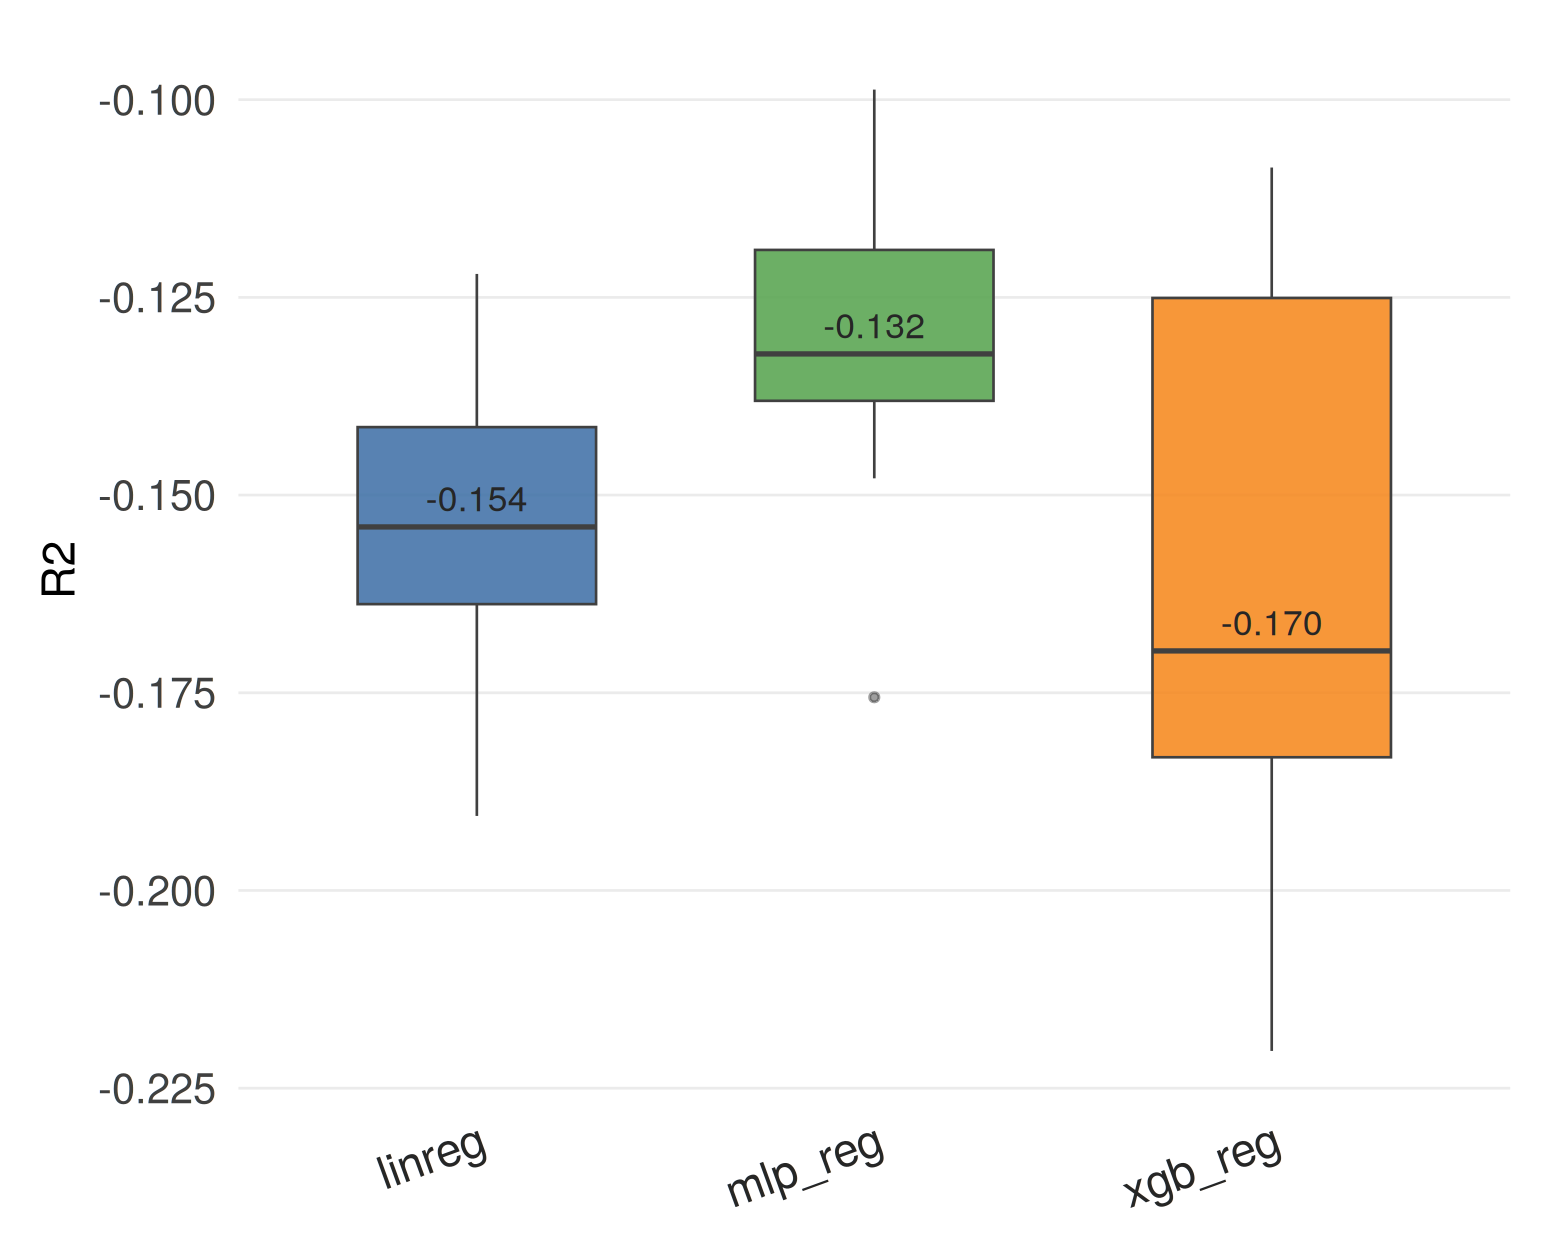
\includegraphics[width=\linewidth]{figures/fig_ap_w_reg_r2_baseline_ibd.png}
    \caption{IBD}
  \end{subfigure}\hfill
  \begin{subfigure}[t]{0.32\textwidth}
    \centering
    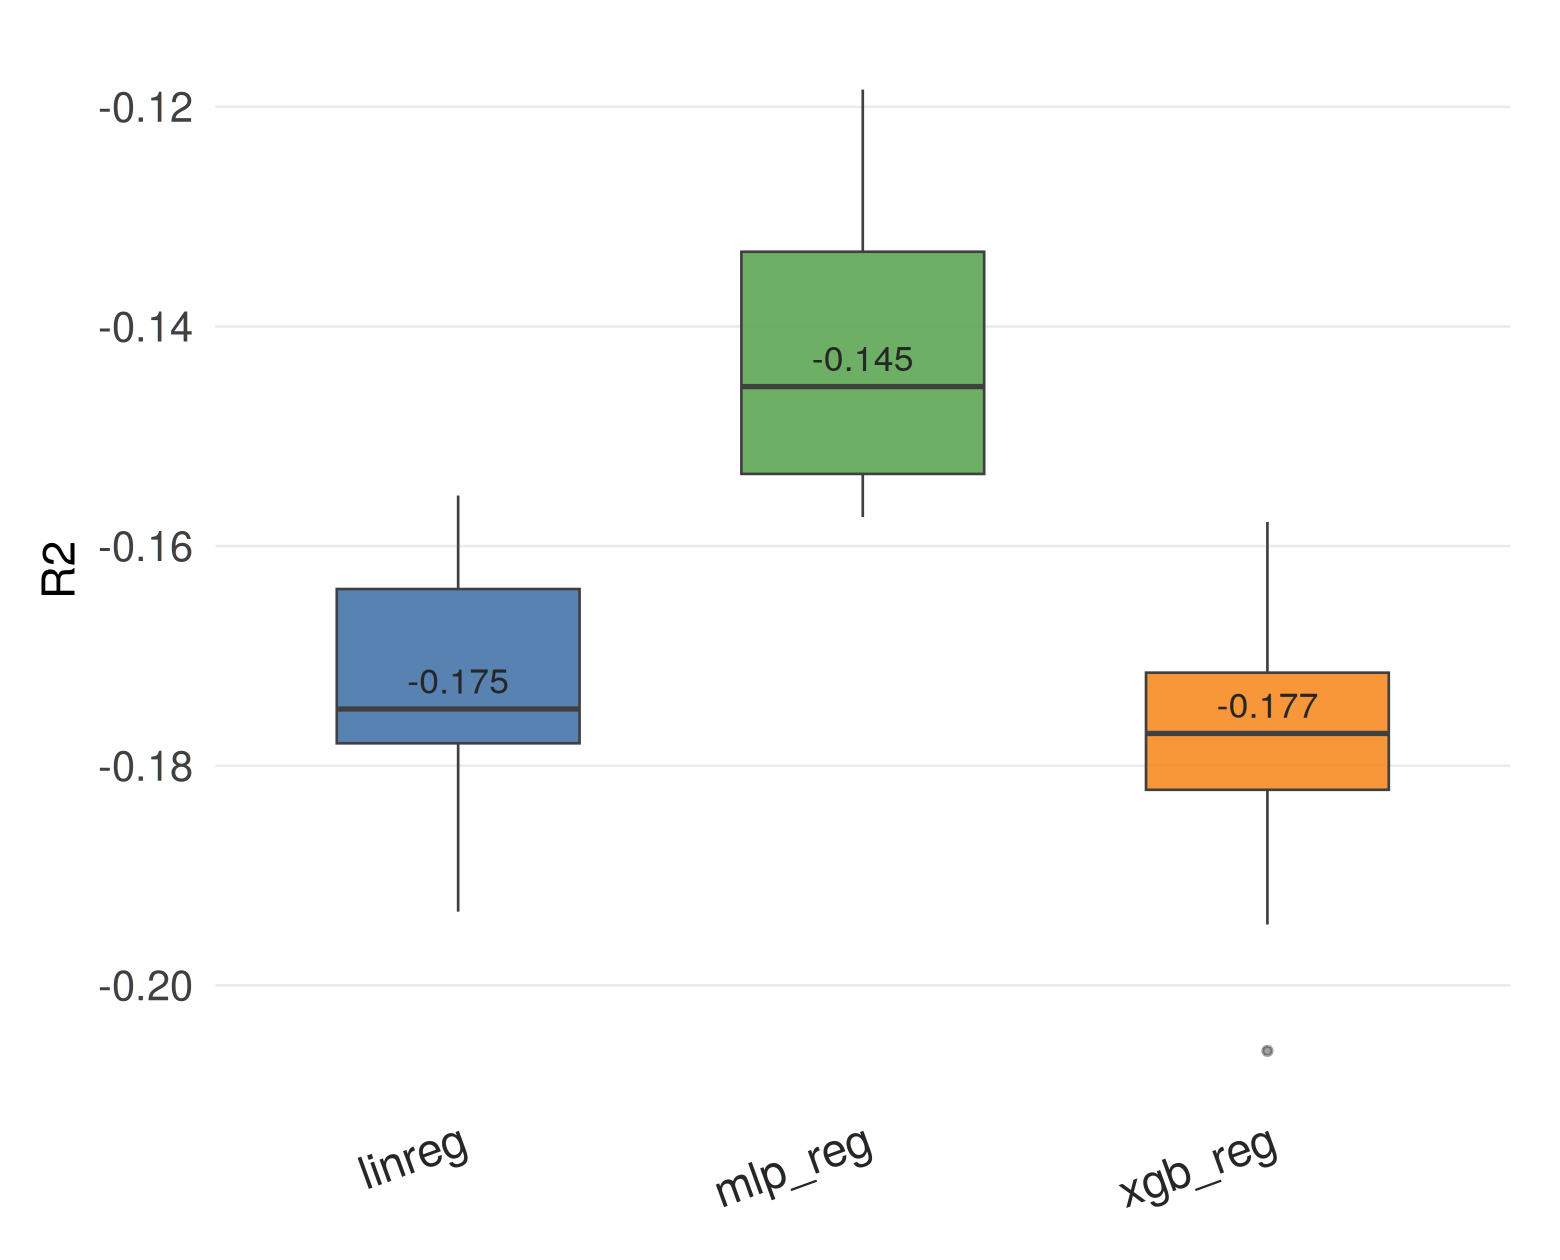
\includegraphics[width=\linewidth]{figures/fig_ap_w_reg_r2_baseline_gvhd.png}
    \caption{GvHD}
  \end{subfigure}
  \caption{Test $R^2$ on the edge selection probability, baseline models}
  \label{fig:ap-wrr2b}
\end{figure}

\begin{figure}[H]
  \centering
  \begin{subfigure}[t]{0.32\textwidth}
    \centering
    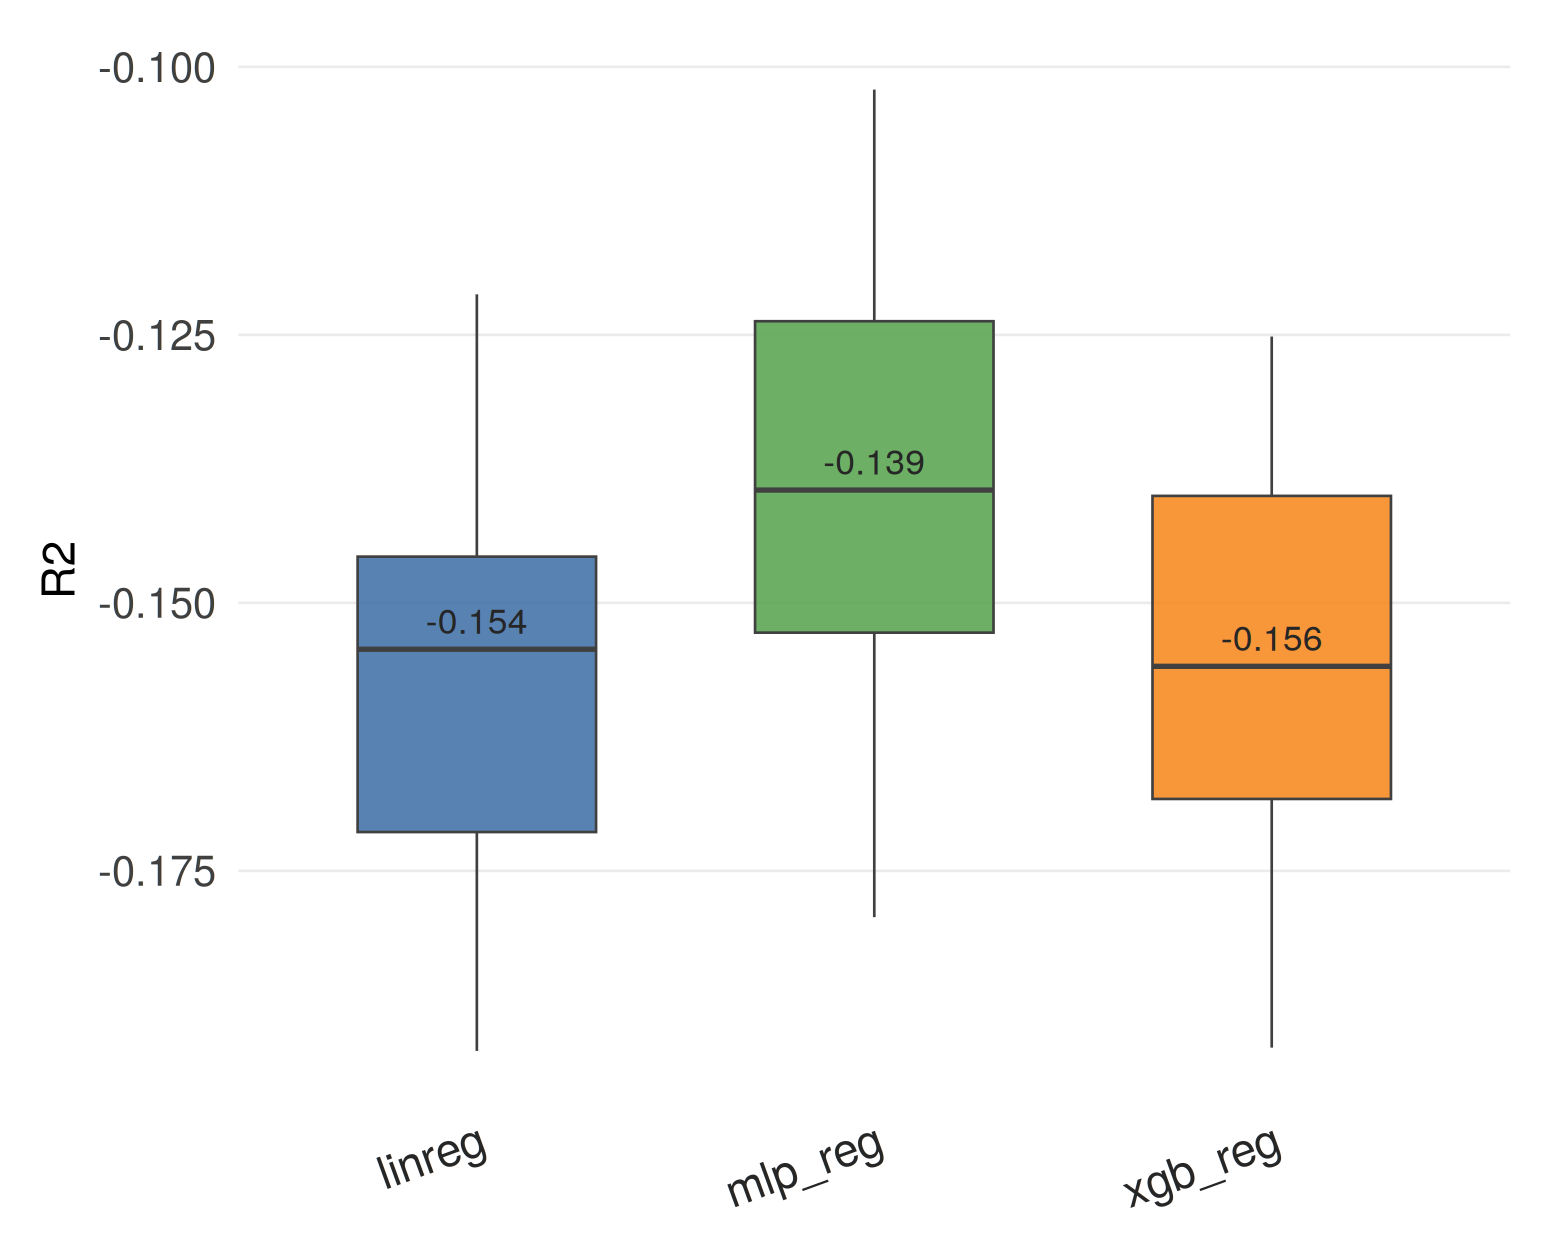
\includegraphics[width=\linewidth]{figures/fig_ap_w_reg_r2_all_crc.png}
    \caption{CRC}
  \end{subfigure}\hfill
  \begin{subfigure}[t]{0.32\textwidth}
    \centering
    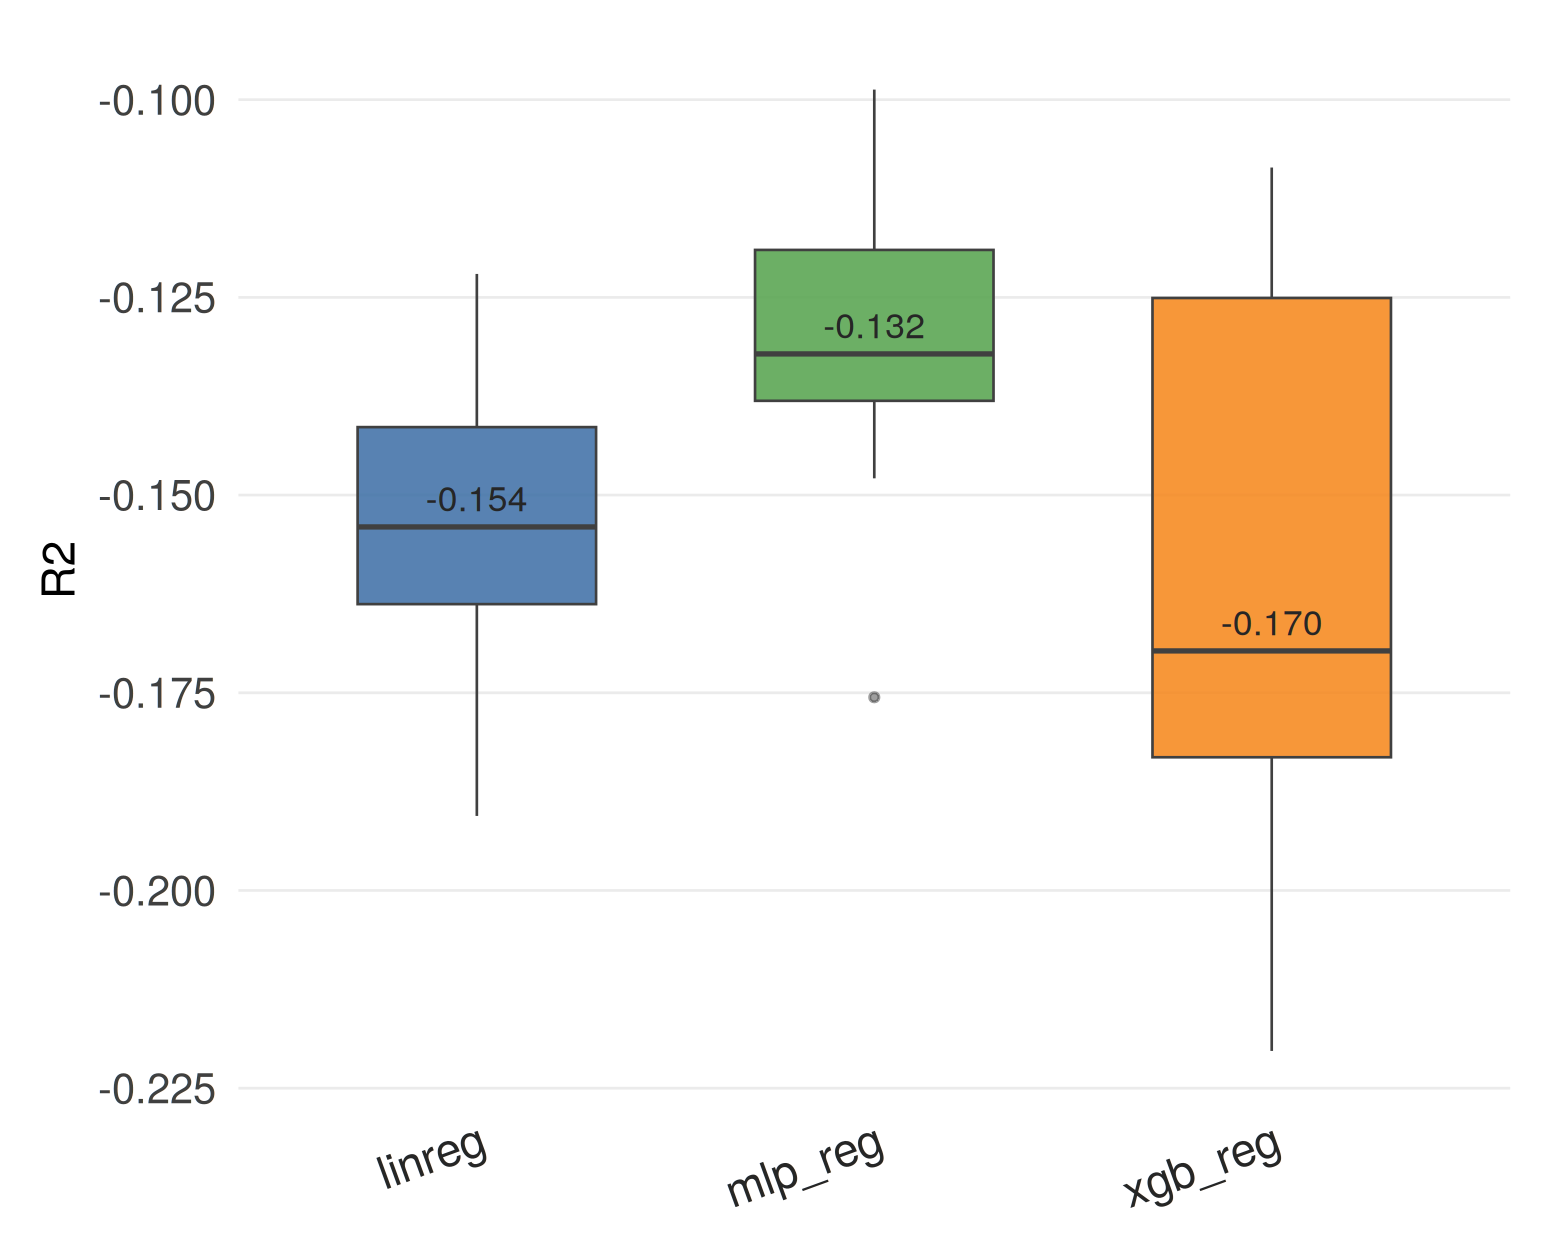
\includegraphics[width=\linewidth]{figures/fig_ap_w_reg_r2_all_ibd.png}
    \caption{IBD}
  \end{subfigure}\hfill
  \begin{subfigure}[t]{0.32\textwidth}
    \centering
    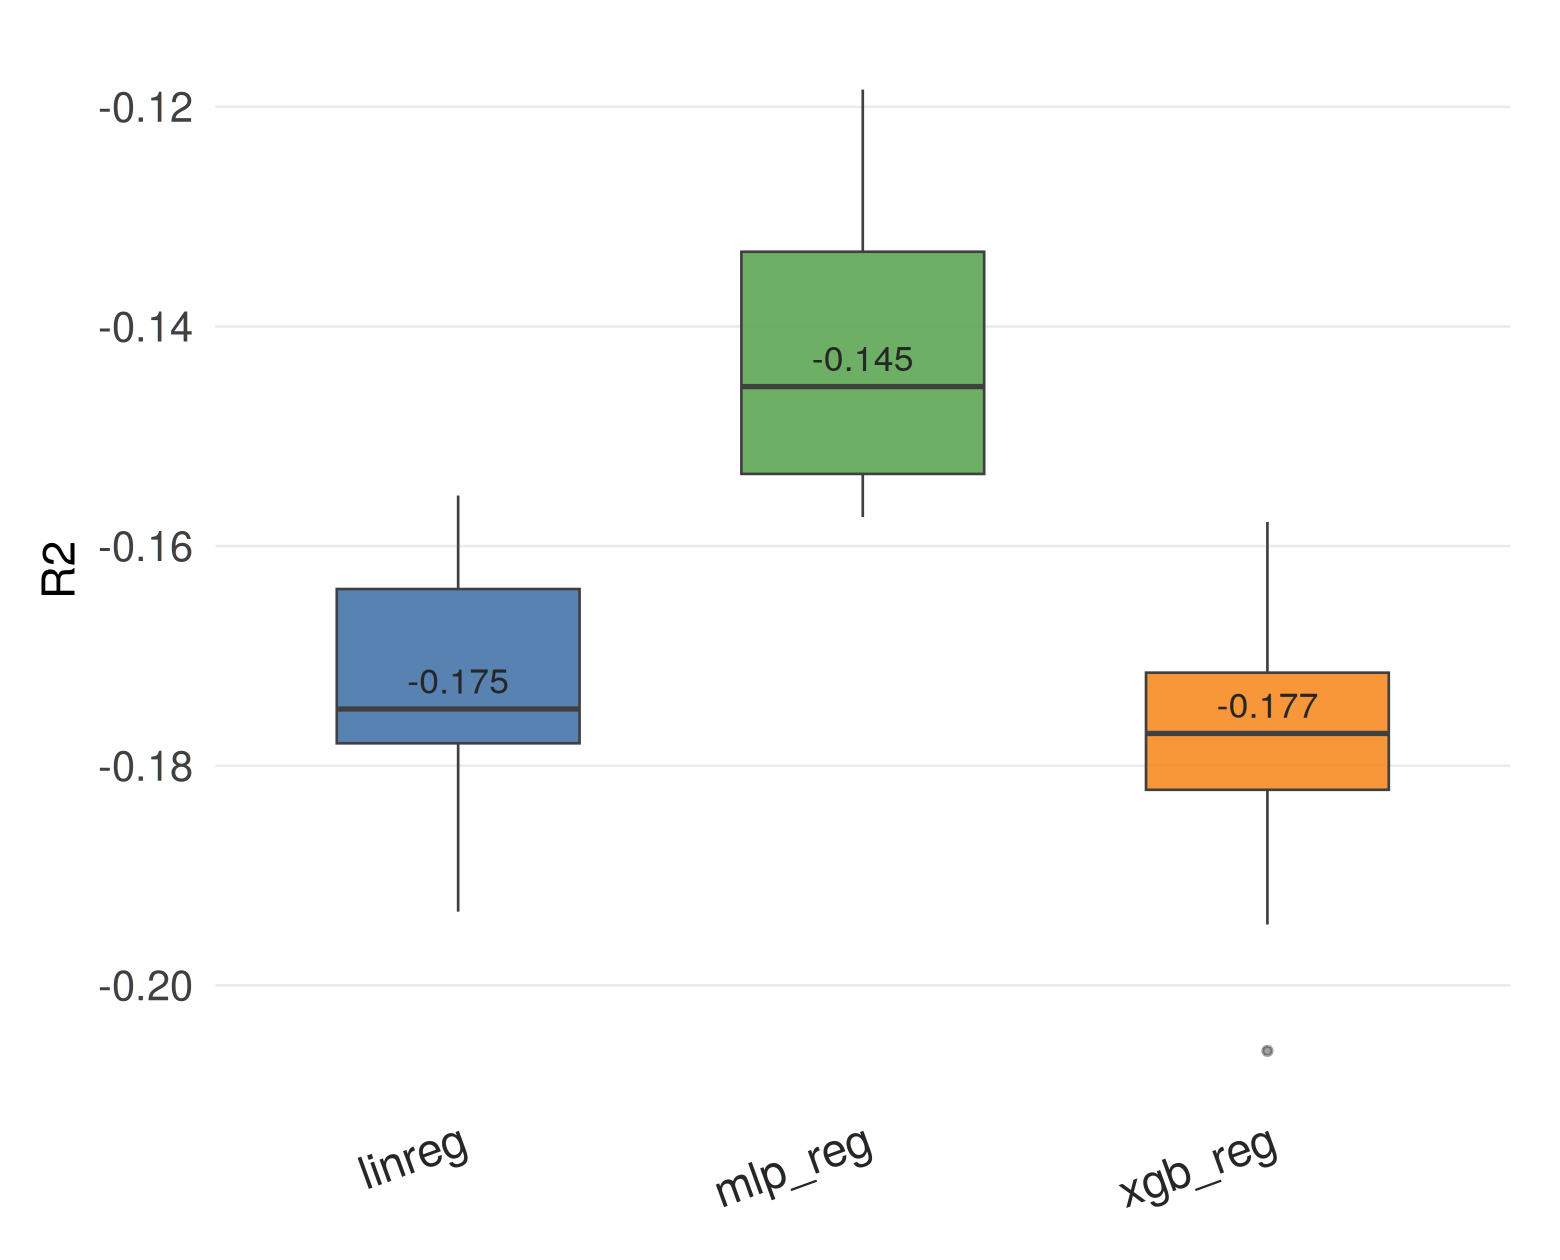
\includegraphics[width=\linewidth]{figures/fig_ap_w_reg_r2_all_gvhd.png}
    \caption{GvHD}
  \end{subfigure}
  \caption{Test $R^2$ on the edge selection probability, all models}
  \label{fig:ap-wrr2a}
\end{figure}

\subsection{Penalty Selection}

\begin{figure}[H]
  \centering
  \begin{subfigure}[t]{0.32\textwidth}
    \centering
    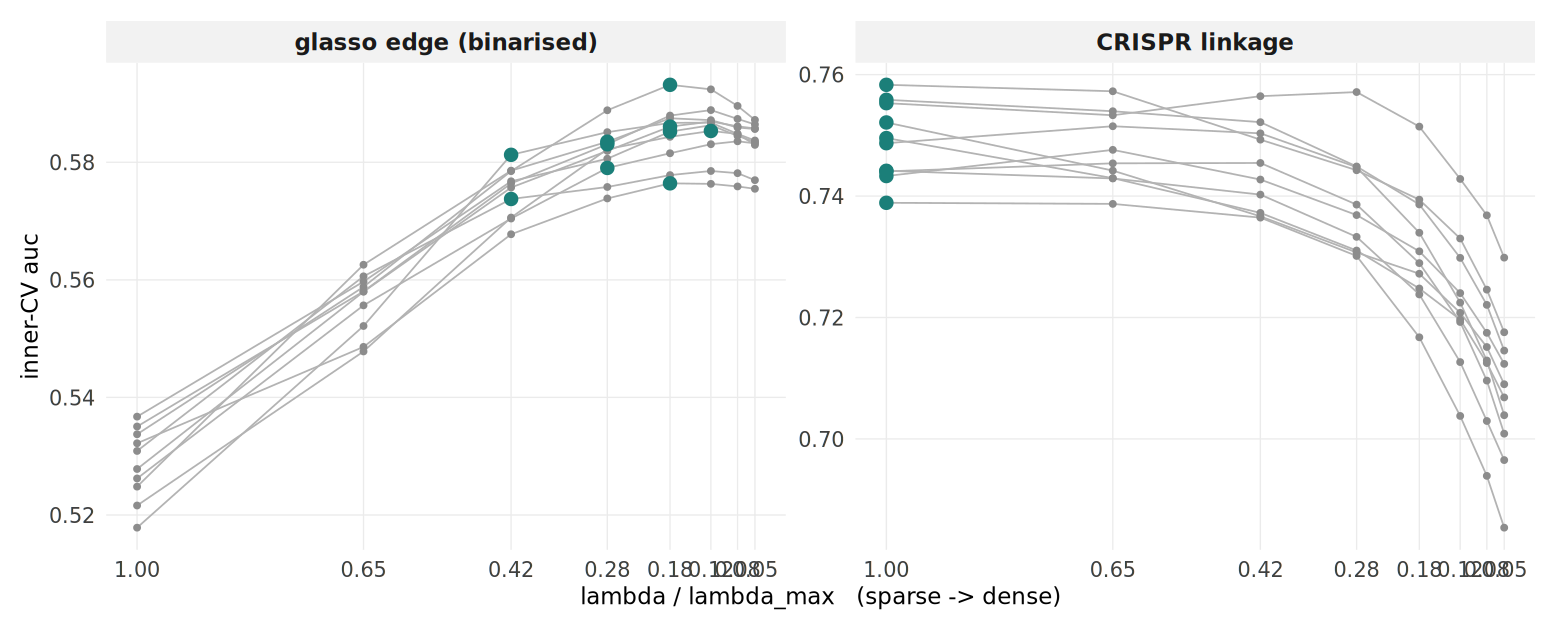
\includegraphics[width=\linewidth]{figures/fig_ap_lambda_cv_curve_crc.png}
    \caption{CRC}
  \end{subfigure}\hfill
  \begin{subfigure}[t]{0.32\textwidth}
    \centering
    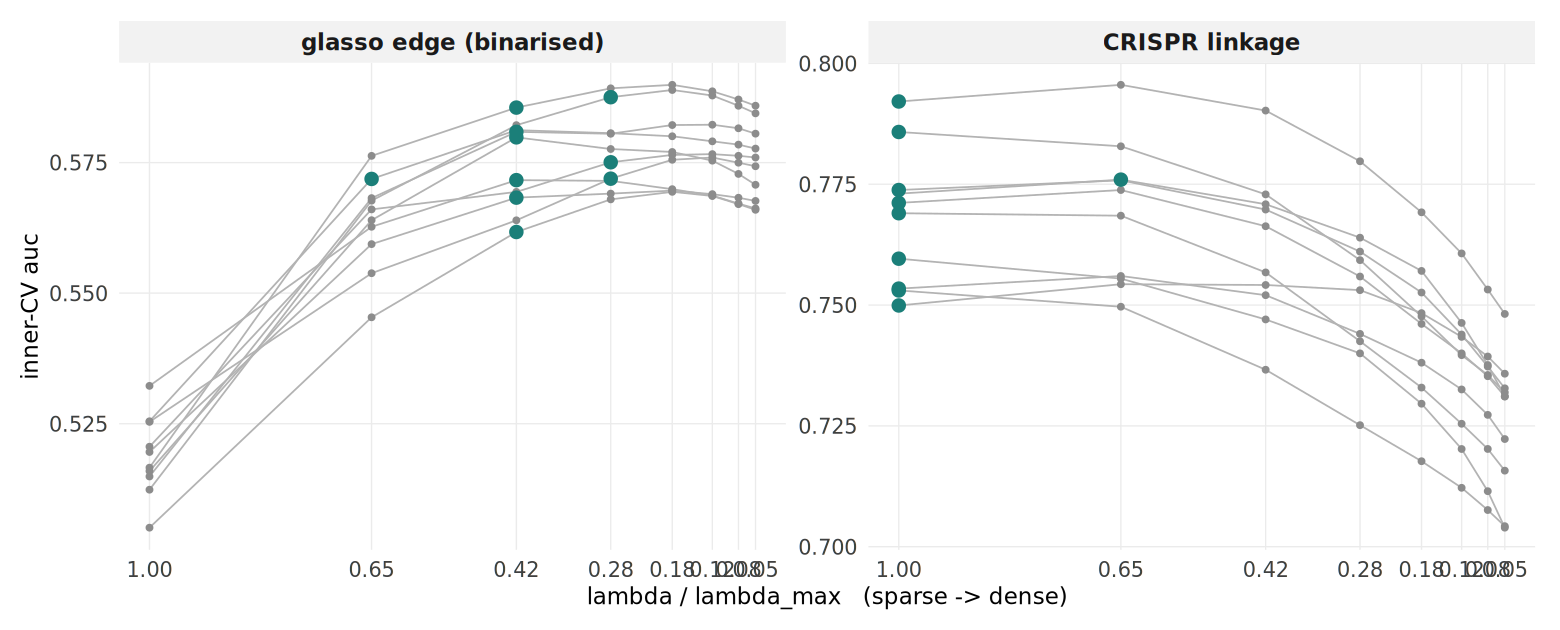
\includegraphics[width=\linewidth]{figures/fig_ap_lambda_cv_curve_ibd.png}
    \caption{IBD}
  \end{subfigure}\hfill
  \begin{subfigure}[t]{0.32\textwidth}
    \centering
    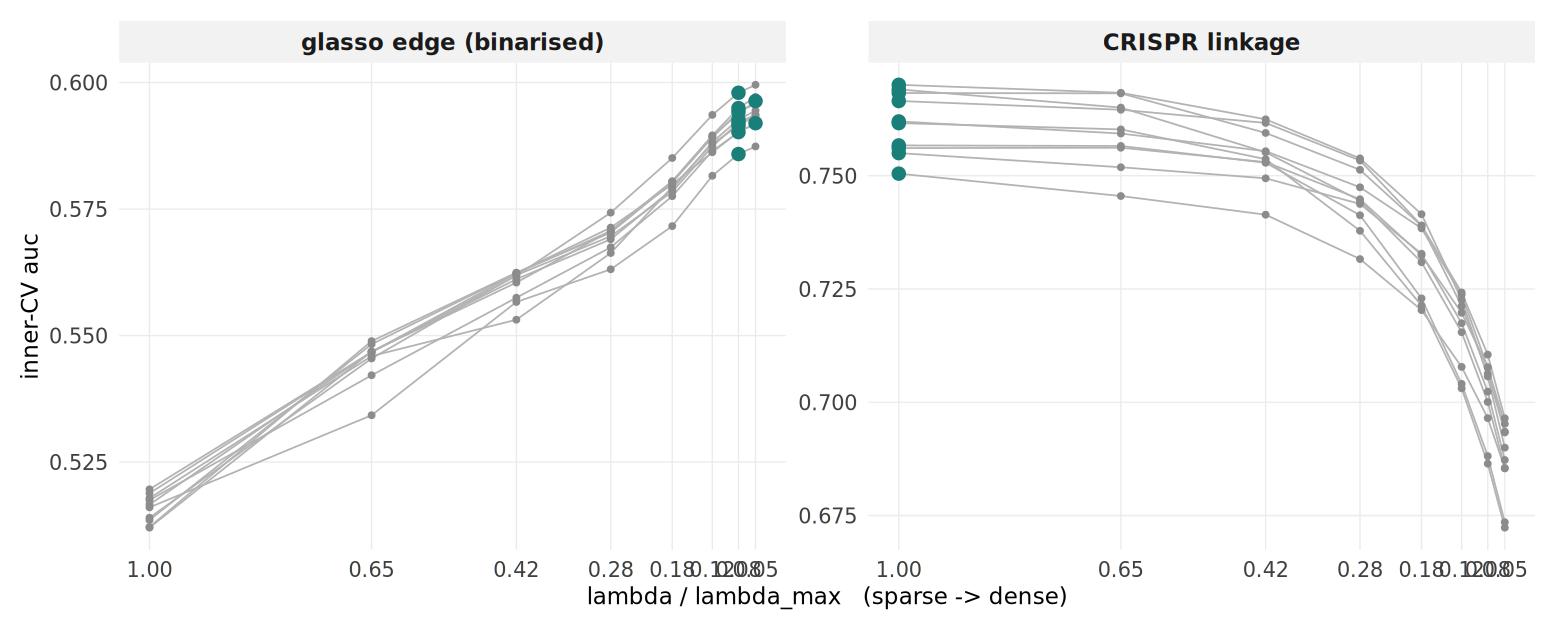
\includegraphics[width=\linewidth]{figures/fig_ap_lambda_cv_curve_gvhd.png}
    \caption{GvHD}
  \end{subfigure}
  \caption{Inner-CV score against the $L_1$ penalty, one line per outer fold}
  \label{fig:ap-lcurve}
\end{figure}

\begin{figure}[H]
  \centering
  \begin{subfigure}[t]{0.32\textwidth}
    \centering
    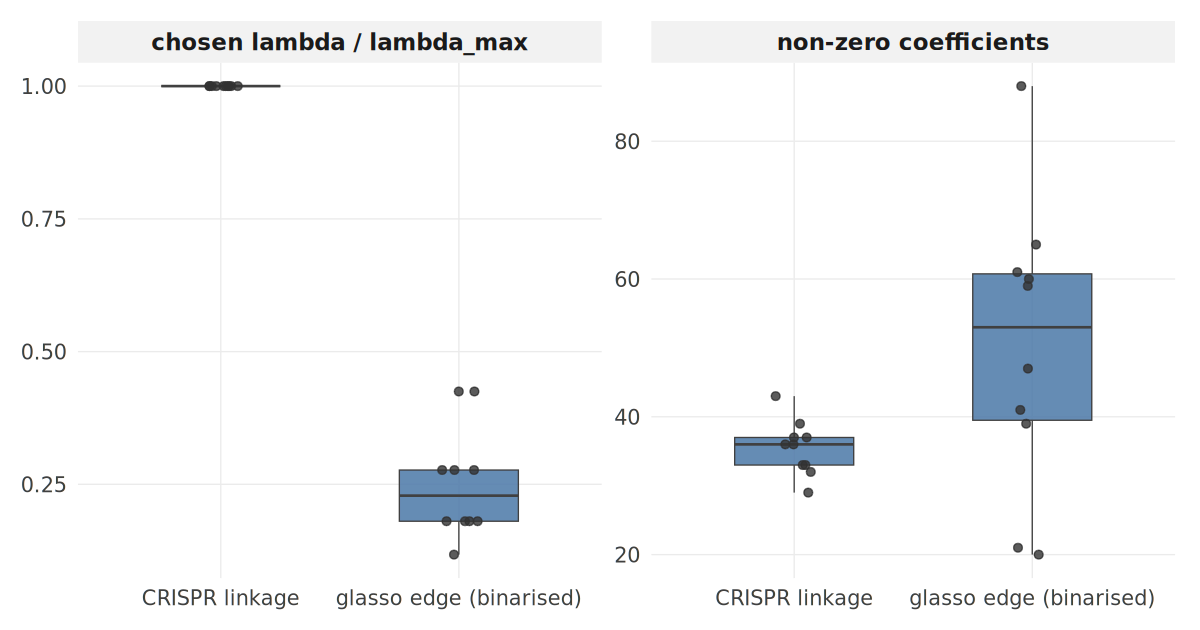
\includegraphics[width=\linewidth]{figures/fig_ap_lambda_cv_choice_crc.png}
    \caption{CRC}
  \end{subfigure}\hfill
  \begin{subfigure}[t]{0.32\textwidth}
    \centering
    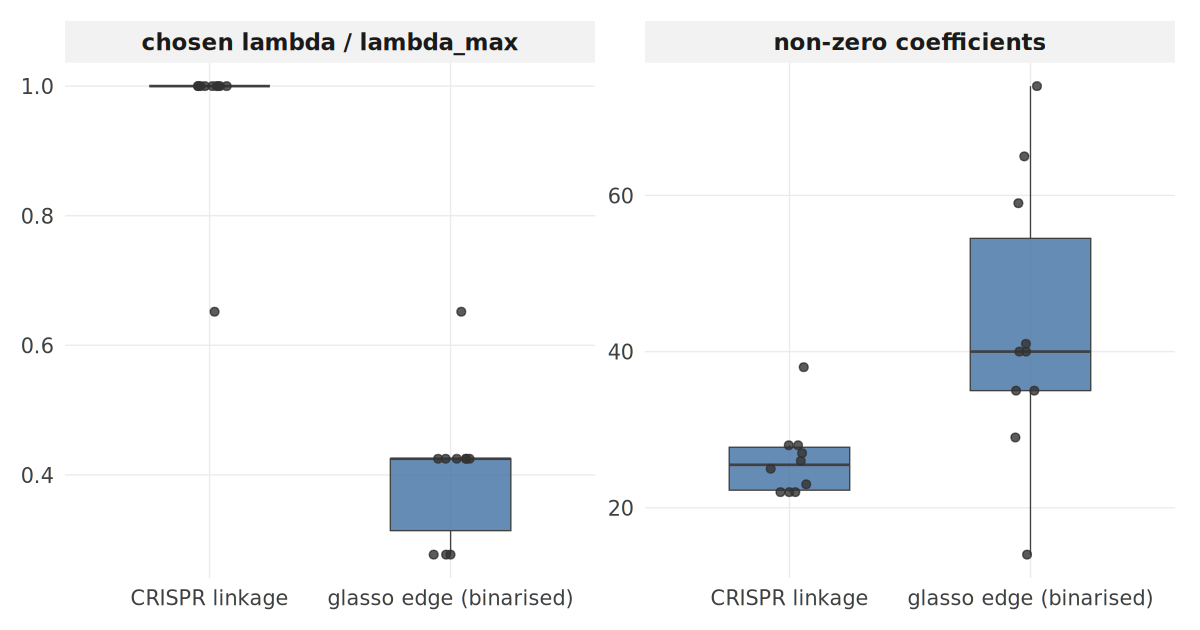
\includegraphics[width=\linewidth]{figures/fig_ap_lambda_cv_choice_ibd.png}
    \caption{IBD}
  \end{subfigure}\hfill
  \begin{subfigure}[t]{0.32\textwidth}
    \centering
    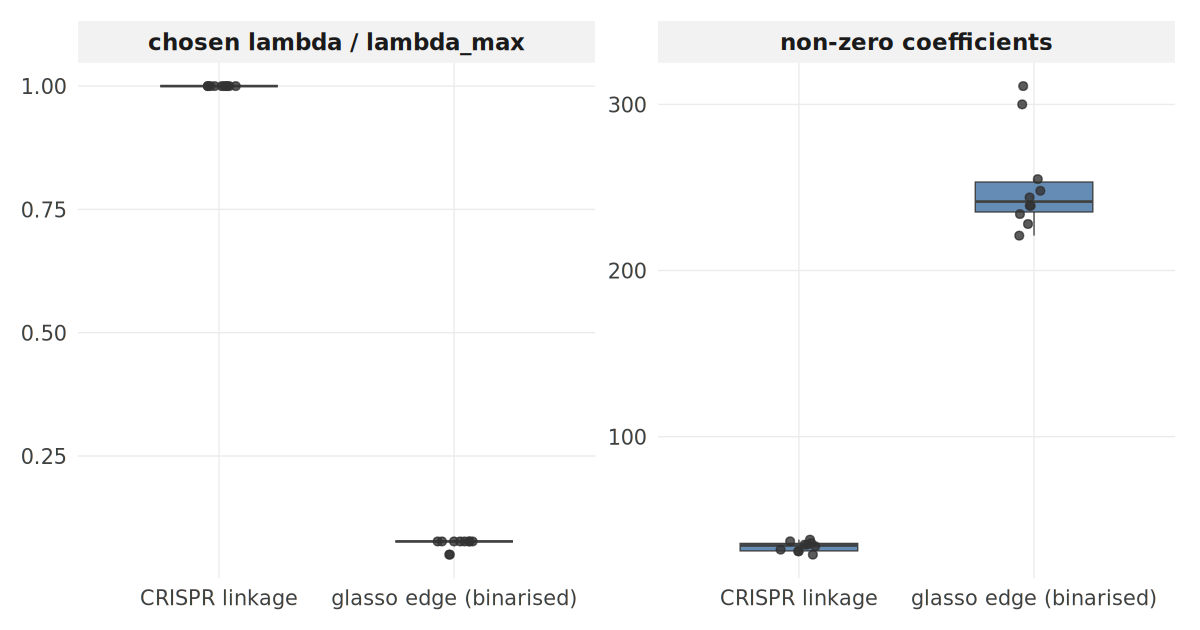
\includegraphics[width=\linewidth]{figures/fig_ap_lambda_cv_choice_gvhd.png}
    \caption{GvHD}
  \end{subfigure}
  \caption{Selected penalty ratio and resulting support size}
  \label{fig:ap-lchoice}
\end{figure}

\subsection{Binarisation Threshold}

\begin{figure}[H]
  \centering
  \begin{subfigure}[t]{0.32\textwidth}
    \centering
    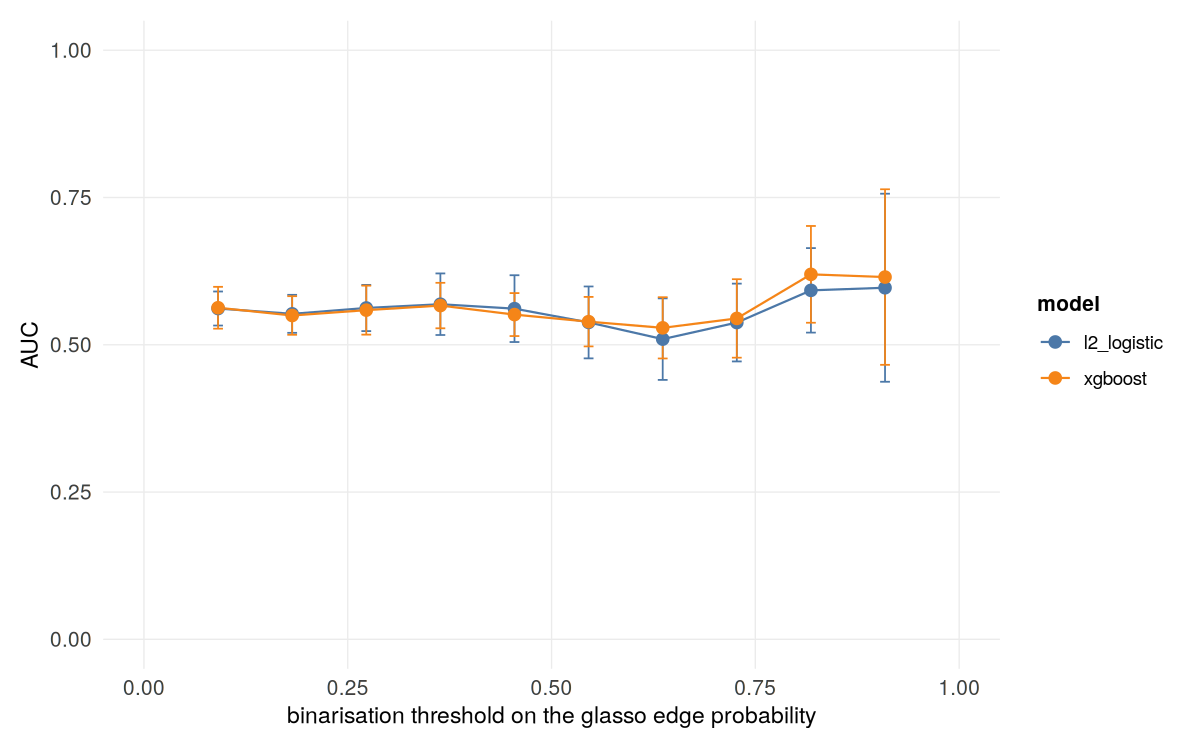
\includegraphics[width=\linewidth]{figures/fig_wthreshold_crc.png}
    \caption{CRC}
  \end{subfigure}\hfill
  \begin{subfigure}[t]{0.32\textwidth}
    \centering
    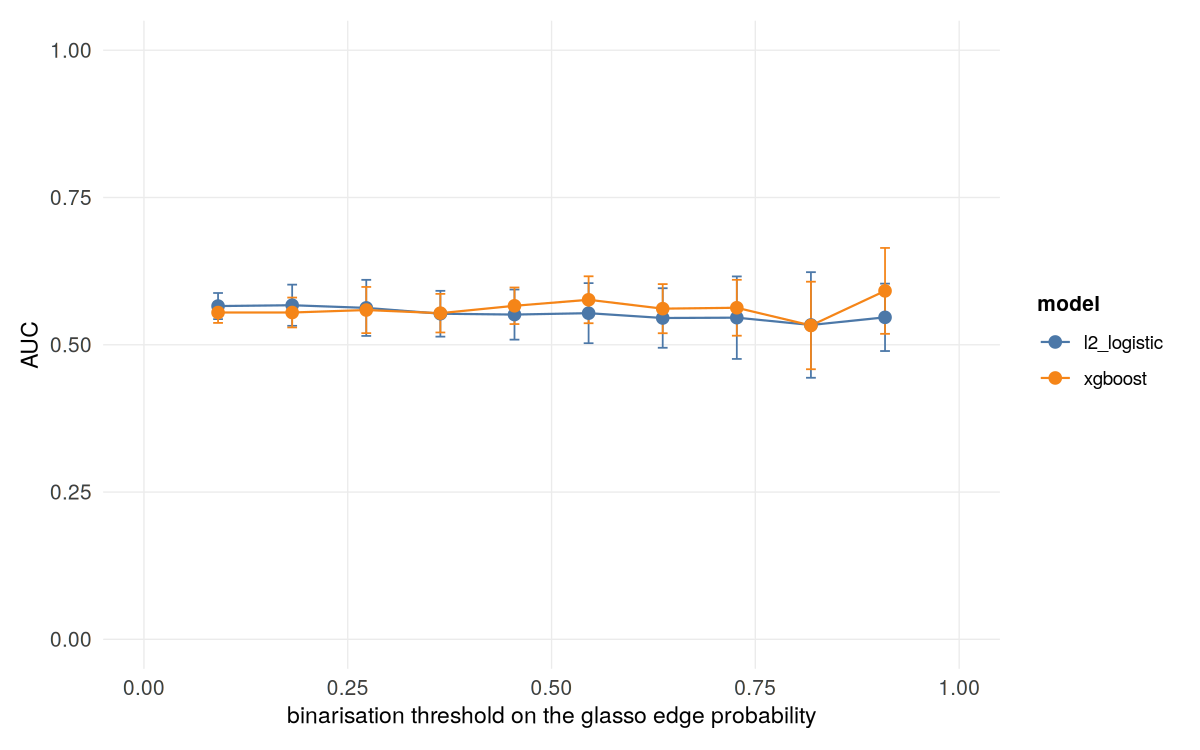
\includegraphics[width=\linewidth]{figures/fig_wthreshold_ibd.png}
    \caption{IBD}
  \end{subfigure}\hfill
  \begin{subfigure}[t]{0.32\textwidth}
    \centering
    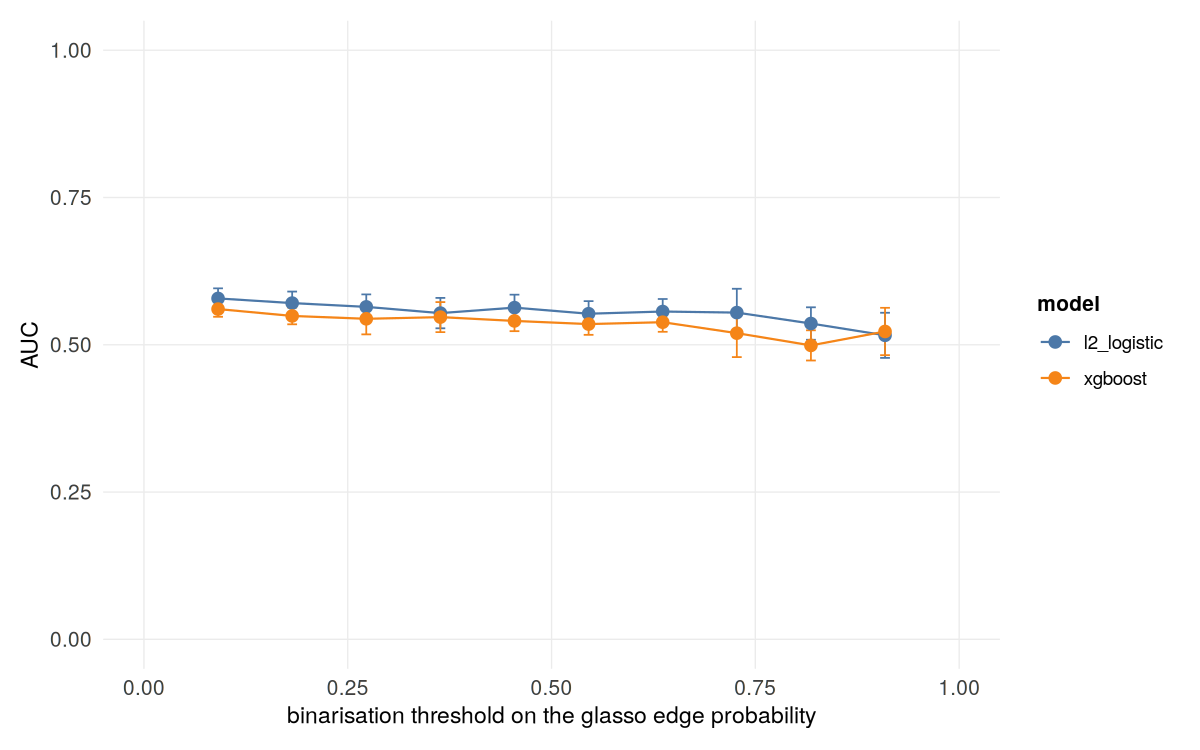
\includegraphics[width=\linewidth]{figures/fig_wthreshold_gvhd.png}
    \caption{GvHD}
  \end{subfigure}
  \caption{Test AUC against the binarisation threshold \(\tau\)}
  \label{fig:ap-wthreshold}
\end{figure}

\subsection{Stability Selection}

\begin{figure}[H]
  \centering
  \begin{subfigure}[t]{0.32\textwidth}
    \centering
    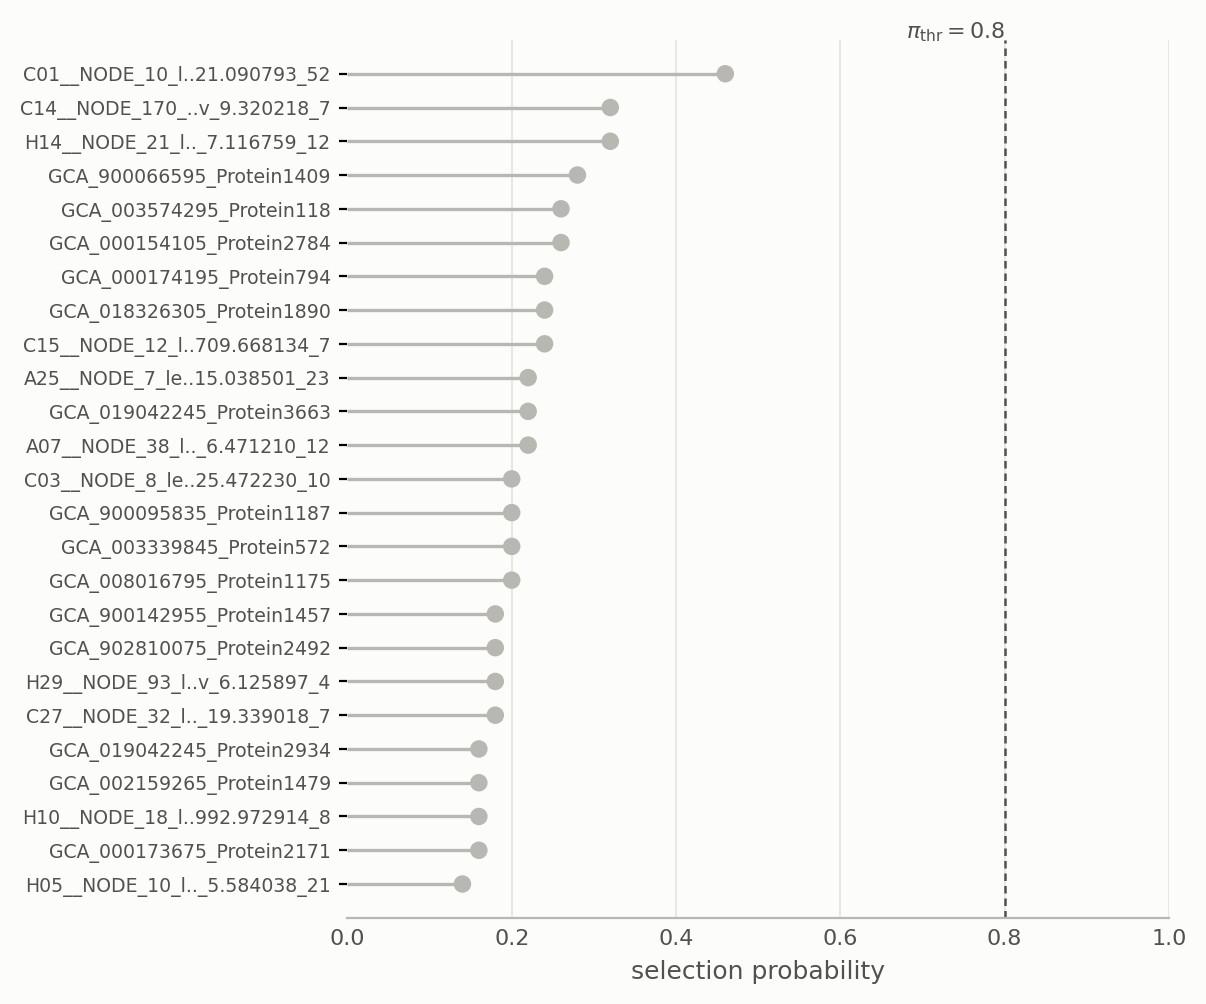
\includegraphics[width=\linewidth]{figures/fig_stability_crc.png}
    \caption{CRC}
  \end{subfigure}\hfill
  \begin{subfigure}[t]{0.32\textwidth}
    \centering
    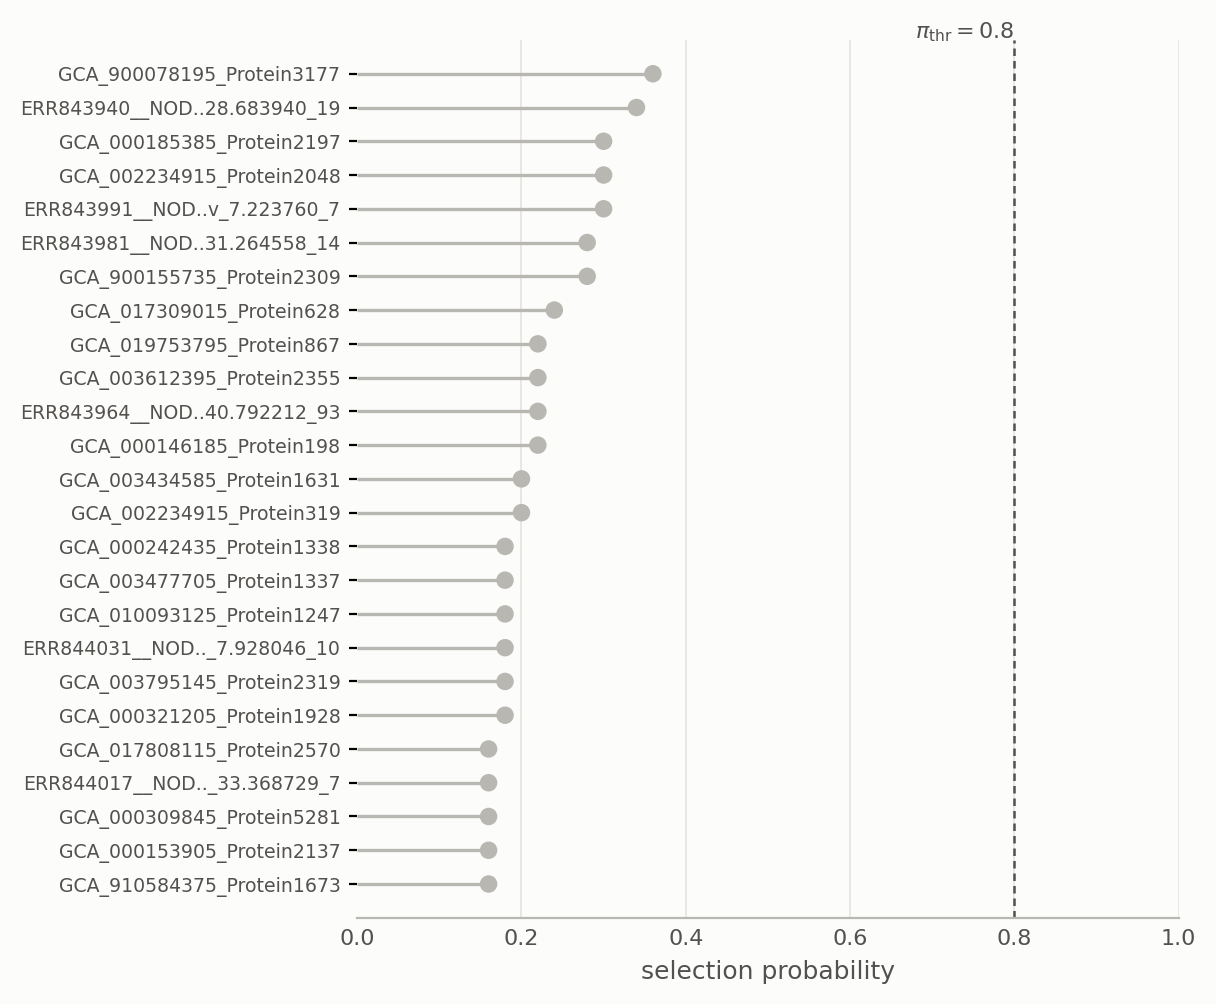
\includegraphics[width=\linewidth]{figures/fig_stability_ibd.png}
    \caption{IBD}
  \end{subfigure}\hfill
  \begin{subfigure}[t]{0.32\textwidth}
    \centering
    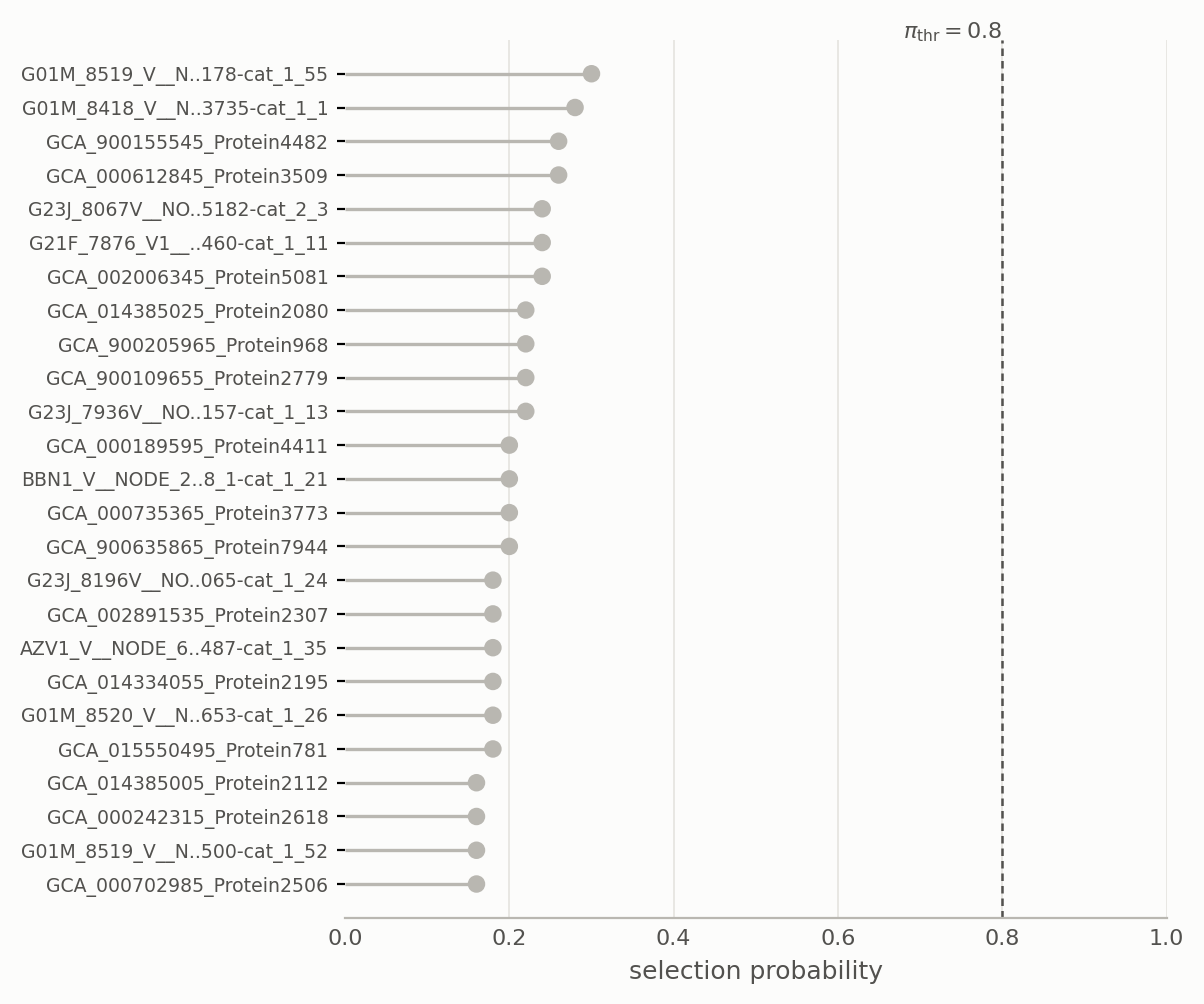
\includegraphics[width=\linewidth]{figures/fig_stability_gvhd.png}
    \caption{GvHD}
  \end{subfigure}
  \caption{Selection probabilities of the 25 highest-ranked protein clusters, with the threshold
  \(\pi_{\mathrm{thr}}=0.8\) marked}
  \label{fig:ap-stab}
\end{figure}

\newpage

\section{Electronic appendix}
\label{el_app}

The electronic appendix accompanies this thesis and contains everything needed to reproduce it. It is
organised in three parts.

\textbf{Code.} The complete pipeline, as a set of independently runnable stages driven by a single
configuration file, together with the R scripts that draw every figure and a README
describing the stage order and the outputs of each stage. The package versions and installation instructions
are included with it.

\textbf{Run outputs.} The three cohort runs on which this thesis is based, one directory per cohort, each
holding the frozen configuration used for that run, the preprocessed protein cluster profiles, the fold assignments, the
per-fold predictions and metrics, and the outputs of the threshold sweep, the latent export, the
representation comparison, the shuffled-$y$ control and the stability selection. All three cohorts were run
under the run identifier \texttt{20260916\_\allowbreak 152830}; every figure and table in this thesis is drawn from that run.

\textbf{Figures.} All figures produced by the pipeline, at the resolution in which they were generated.
Section~\ref{app} reproduces every one of them that is not already shown in Section~\ref{results}.

\newpage

% ------------------------------------------------------------------------------
% BIBLIOGRAPHY -----------------------------------------------------------------
% ------------------------------------------------------------------------------

\RaggedRight
\bibliography{bibliography}
\bibliographystyle{dcu}
\newpage

% ------------------------------------------------------------------------------
% DECLARATION OF AUTHORSHIP-----------------------------------------------------
% ------------------------------------------------------------------------------

\Large
\noindent
\textbf{Declaration of authorship}
\vspace{0.5cm}
\noindent
\normalsize

I hereby declare that the report submitted is my own unaided work. All direct
or indirect sources used are acknowledged as references. I am aware that the
Thesis in digital form can be examined for the use of unauthorized aid and in
order to determine whether the report as a whole or parts incorporated in it may
be deemed as plagiarism. For the comparison of my work with existing sources I
agree that it shall be entered in a database where it shall also remain after
examination, to enable comparison with future Theses submitted. Further rights
of reproduction and usage, however, are not granted here. This paper was not
previously presented to another examination board and has not been published.
\\

\vspace{1cm}

\Large
\noindent
\textbf{Declaration on the use of AI tools}
\vspace{0.5cm}
\noindent
\normalsize

I hereby confirm that I have written all parts of this text myself. I used Claude
(Opus 4.8 and Opus 5, Cowork; Anthropic) and ChatGPT (GPT-5.6; OpenAI) as tools. The source code of
the analysis pipeline was generated with Claude under my direction, and I further used Claude for
restructuring and refining the writing, for checking the analysis for errors, and for literature
search. ChatGPT was used for restructuring and refining the writing. I specified the
experimental design, the structure of the pipeline and every analytical choice, reviewed each
stage and inspected its outputs. All suggestions were manually reviewed, adapted and reformulated,
and I take full responsibility for the content of this work.
\\

\vspace{1cm}
\textcolor{orange}{Location, date} \\

\vspace{3cm}

\noindent\rule{0.5\textwidth}{0.4pt} \\

\myname

% ------------------------------------------------------------------------------

\end{document}
